\chapter{Results and Discussion}
\label{ch:results}
This chapter presents the main results and findings from all experiments defined in the previous Chapter \ref{ch:experiments}. First a short revisit of the results from the Best Channel Study is given in Section \ref{sec:results_best_channel}, as the best channels are used in the further experiments.

The main results and their discussion of this thesis begin in Sections \ref{sec:results_benchmark1} to \ref{sec:results_benchmark3} with the three Benchmarks, to test the PatchTST classifiers ability to generalize to unseen dataset domains. Benchmark 1 assigns the testset over all domains, Benchmark 2 to specific \texttt{rod\_type + tolerance} domains and Benchmark 3 assigns the testset individually to all domain-attributes for a broader held-out testset.

After the Benchmark results follow the results and discussion from the Deviation Analysis I and II in Sections \ref{sec:results_deviation_analysis_1} and \ref{sec:results_deviation_analysis_2}, which aim to investigate how certain deviations applied to the insertions, affect physical success outcome, and which deviations produce ambiguous insertion signals that confuse the models ability to classify correctly.

In the end a summary of the main findings is given.


% MARK: Best Channel Study
\section{Best Channel Study}
\label{sec:results_best_channel}
The Best Channel Study was conducted as a standalone study as the first Experiment in Section \ref{sec:exp1_best_channel_study} with its own Motivation, Methods, Results, Discussion and Conclusion.
The recorded dataset contains these signal modalities: force/torque, TCP pose, TCP velocity, joint pose, joint velocity, tool acceleration, per-joint current consumption, and temperature readings per joint.

Stage 1 evaluated each individual channel group with the \texttt{Base} PatchTST model and selected force/torque, TCP pose, joint velocity and current consumption as the strongest signals based on validation balanced accuracy. Refer to \figref{fig:best_channel_single_val_bal_acc} and \figref{fig:best_channel_single_val_loss} in Section \ref{sec:best_channel_study_results} for the detailed comparison.

Stage 2 combined the selected channel groups in all $4\times4=16$ possible ways, with training being done with the \texttt{Big} PatchTST model, in order to better represent the higher dimensional and information rich data in latent space. All $16$ tested channel combinations are shown in an odered binary counting pattern in \figref{fig:results_BCS_comparison}. Light blue highlighted rows mark the single channel groups. \tabref{tab:best_channels_in_detail} shows the validation balanced accuracy from the selected best channels individually and as a combined group.

The best channel study shows that FT is the strongest individual channel group based on mean validation balanced accuracy in \tabref{tab:best_channels_in_detail}, but that the highest performance is obtained when FT is combined with additional robot-state modalities. In particular, current, TCP pose, and joint velocity provide complementary information about actuator load, geometric state, and motion dynamics. Based on these results, the combination of F/T, TCP pose, joint velocity, and current is used for the following benchmark experiments.

\begin{figure}[htpb]
    \centering
    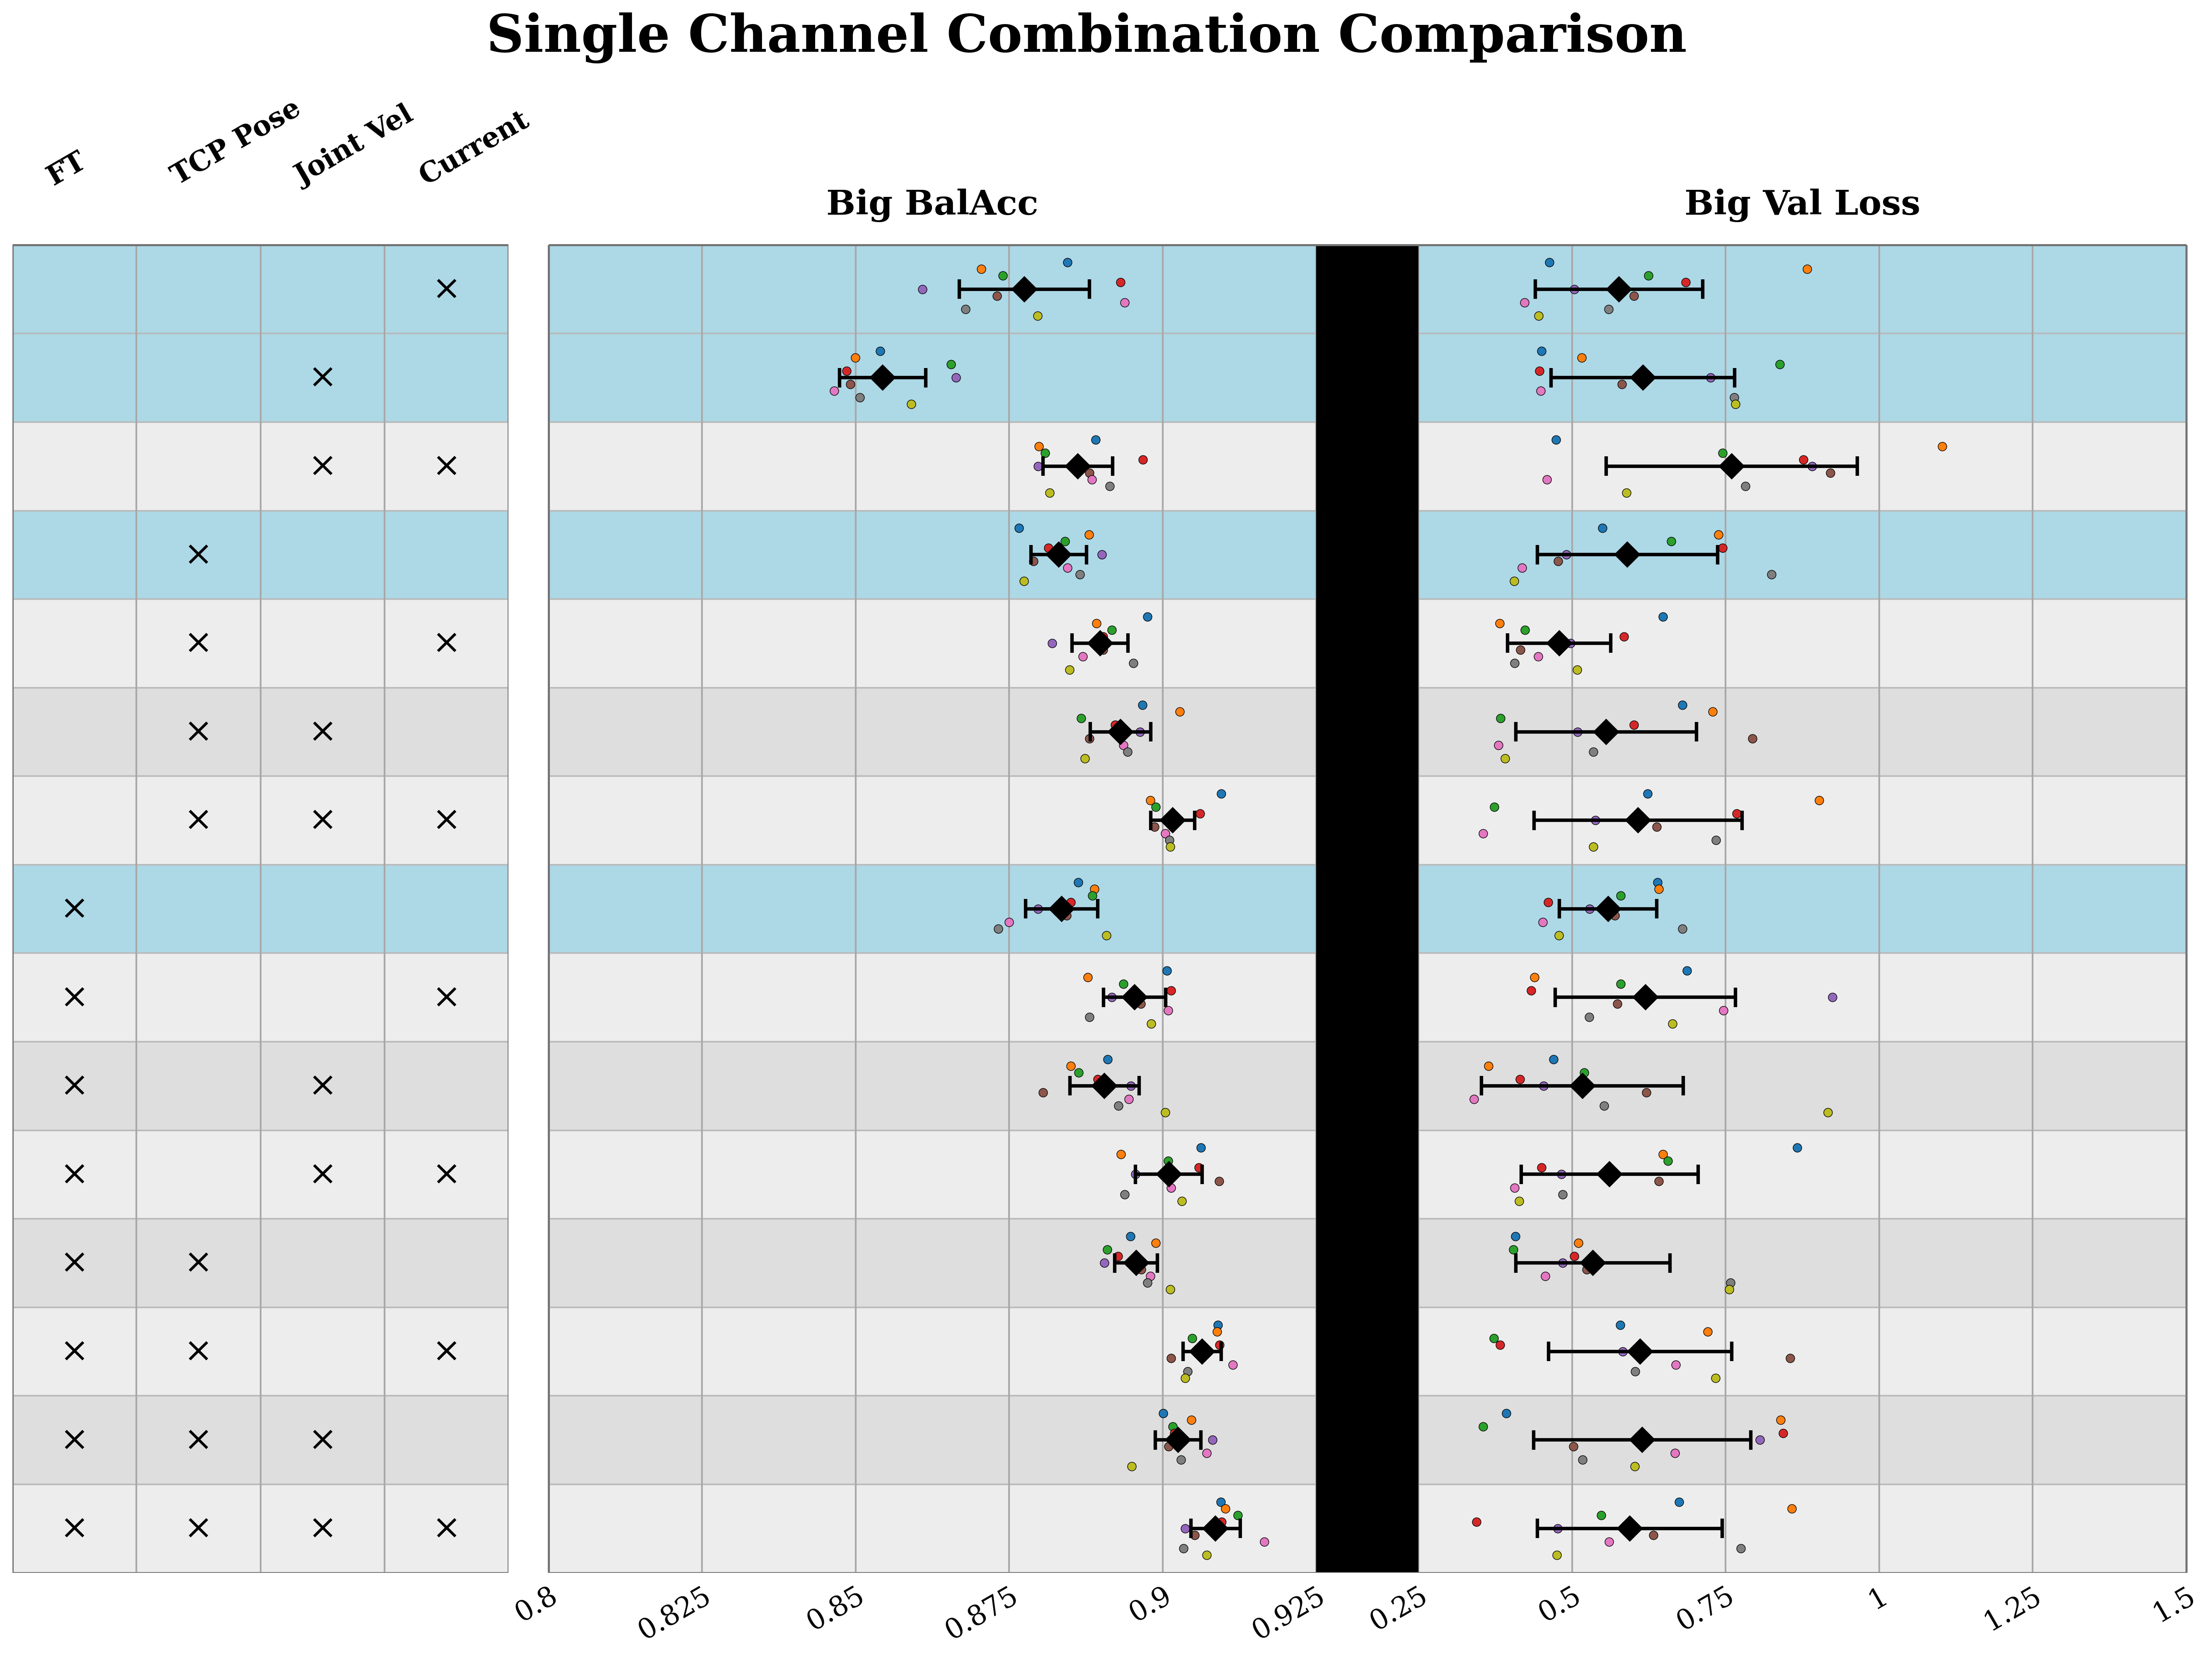
\includegraphics[width=1.0\textwidth]{chapters/7-results_and_discussion/best_channel_study/channel_matrix_plot.png}
    \caption{All combinations of the selected best channels evaluated with the \texttt{Big} model on validation balanced accuracy and validation loss across the 9 training run seed combinations. Rows highlighted in light blue mark the single channel groups.}
    \label{fig:results_BCS_comparison}
\end{figure}

\begin{table}[htbp]
    \centering
    \caption{Best channels selected with detailed view on validation balanced accuracy across the 9 training runs. ms: model seed, ss: split seed.}
    \label{tab:best_channels_in_detail}
    \begin{tabular}{llll}
        \toprule
        \textbf{Channel} & \textbf{Mean $\pm$ std} & \textbf{Min (ms, ss)} & \textbf{Max (ms, ss)}\\
        \midrule

        \texttt{FT} & 0.8859 $\pm$ 0.0075 & 0.8716 (420,69) & 0.8930 (420,420)\\
        \texttt{TCP\_POS} & 0.8854 $\pm$ 0.0053 & 0.8782 (42,42) & 0.8932 (69,69) \\
        \texttt{JOINT\_VEL} & 0.8535 $\pm$ 0.0083 & 0.8447 (420,42) & 0.8667 (69,69) \\
        \texttt{CURRENT} & 0.8792 $\pm$ 0.0125 & 0.8607 (69,69) & 0.8974 (420,42) \\
        \texttt{FT} + \texttt{TCP\_POS} + \texttt{JOINT\_VEL} + \texttt{CURRENT} & 0.9139 $\pm$ 0.0047 & 0.9081 (420,69) & 0.9227 (420,42)\\
        \bottomrule
    \end{tabular}
\end{table}


\newpage
% MARK: BM1
\section{Benchmark 1: Test on Mixed Split}
\label{sec:results_benchmark1}
Benchmark 1 evaluates the selected channel configuration under an in-distribution split, where the test samples are unseen insertion attempts but originate from the same overall experimental domain as the training data. This testset is evaluated on the
\begin{itemize}
    \item Base config: \texttt{Base} PatchTST model with \texttt{FT} as the only input data and
    \item Big config: \texttt{Big} PatchTST model with the best channels \texttt{FT + TCP\_POS + JOINT\_VEL + CURRENT} as input data.
\end{itemize}

The number of sequences and class balance of the training, validation and test split is shown in \tabref{tab:bm1_data_split}. The split is close to balanced in all subsets, with 659 positive and 556 negative samples in the test set.

The test balanced accuracy (TBA) in \figref{fig:bm1_test_result} (a) is high for both model variants. The Base config reaches a mean TBA of 0.8617, while the Big config reaches 0.8909 (\tabref{tab:bm1_bal_acc_detail}). This corresponds to an improvement of 0.0292 TBA points for the Big config. The improvement is also consistent across the evaluated seed combinations. The lowest TBA from one seed combination on the Big config is 0.8816, which is still higher than the highest TBA from one seed combination on the Base config with 0.8768. In addition, the standard deviation is lower for the Big config. This indicates that the combination of the larger model and the selected channel groups does not only improve the mean result, but also makes the balanced accuracy less dependent on the specific seed combination and therefore more reliable.

The test loss in \figref{fig:bm1_test_result} (b) shows a different pattern. The Base config has a lower mean test loss and a smaller spread across seeds, while the Big config shows a higher mean loss and larger variability. This does not contradict the balanced-accuracy result, because the two metrics describe different properties of the classifier. Balanced accuracy evaluates the final class decision after converting the model output into a binary prediction, whereas the loss also penalizes the confidence of the predicted probabilities. The Big config therefore separates the two classes more successfully in terms of the final classification, but its predicted probabilities are less stable across seeds.

For Benchmark 1, the main conclusion is therefore that the Big config provides the stronger in-distribution classifier, but not the better calibrated one. Since this benchmark uses a mixed split, the result should be interpreted as a baseline/control group performance under favorable conditions, not as evidence for generalization to unseen domains. Its main purpose is to define the reference level for the more difficult domain-shift experiments in Benchmark 2 and Benchmark 3.
\begin{figure}[htbp]
    \centering
    \begin{subfigure}[t]{0.49\textwidth}
        \centering
        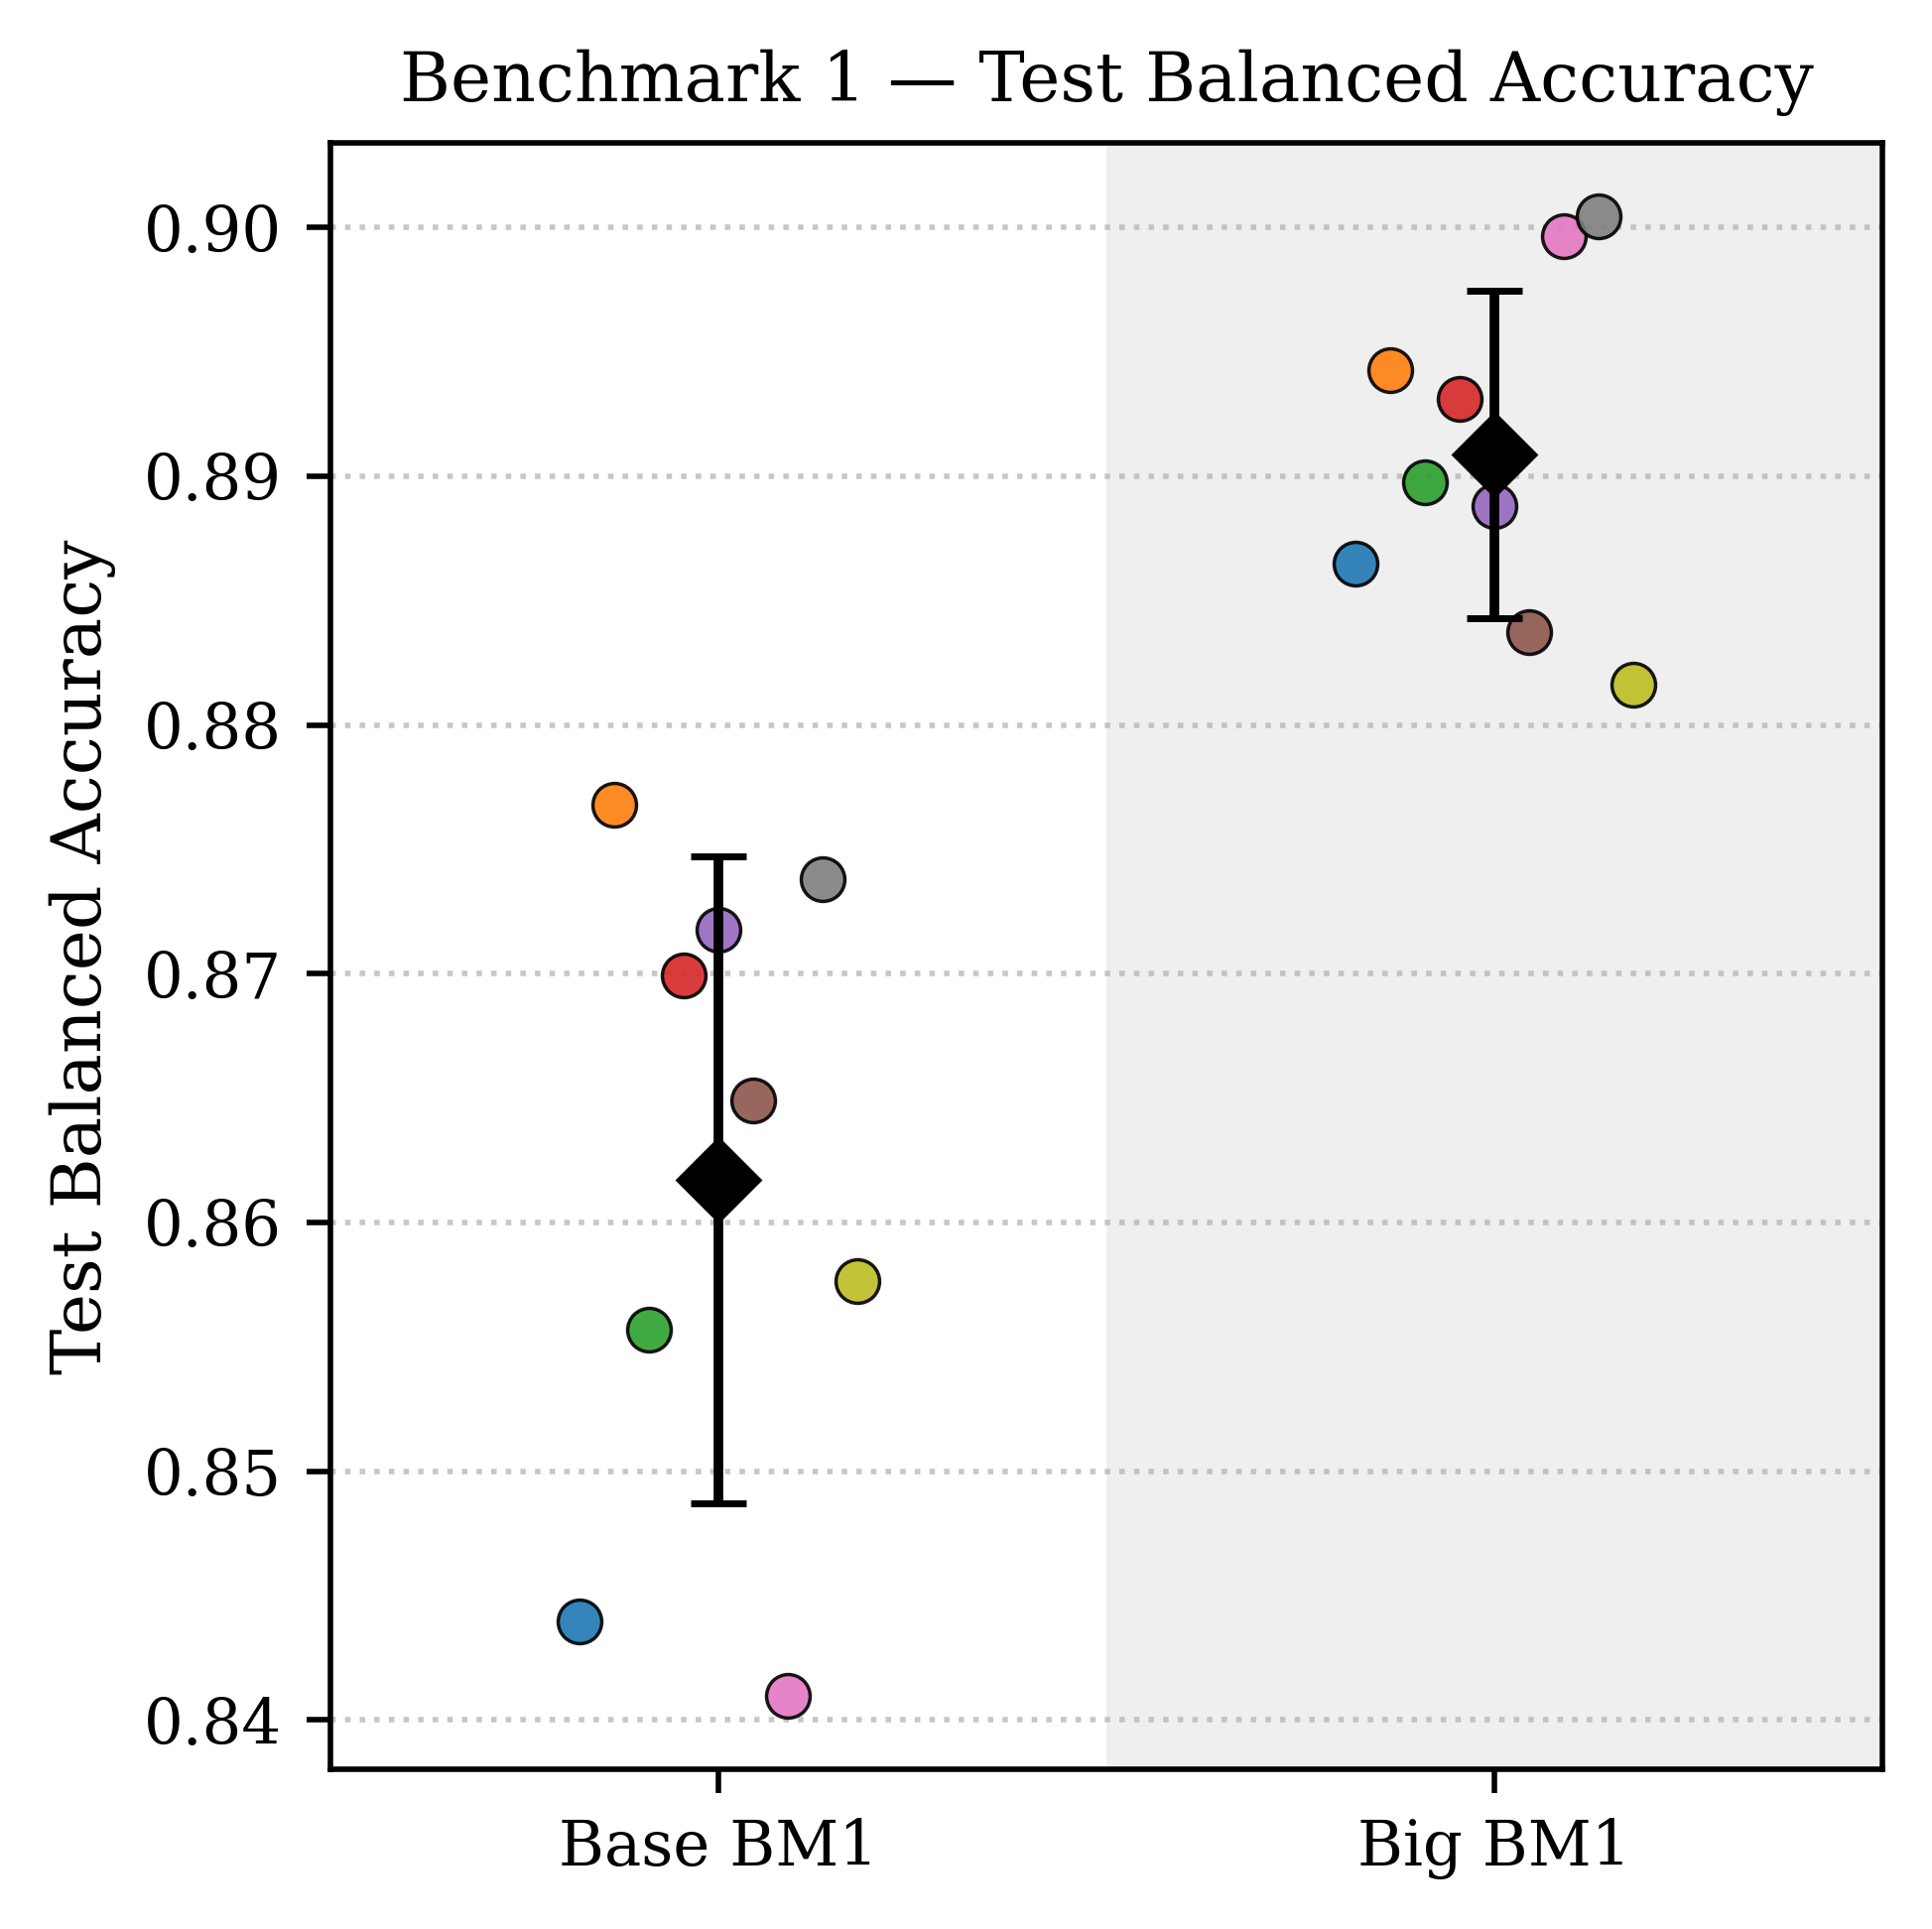
\includegraphics[width=0.9\textwidth]{chapters/7-results_and_discussion/bm1/bm1_bal_acc.png}
        \caption{}
    \end{subfigure}
    \begin{subfigure}[t]{0.49\textwidth}
        \centering
        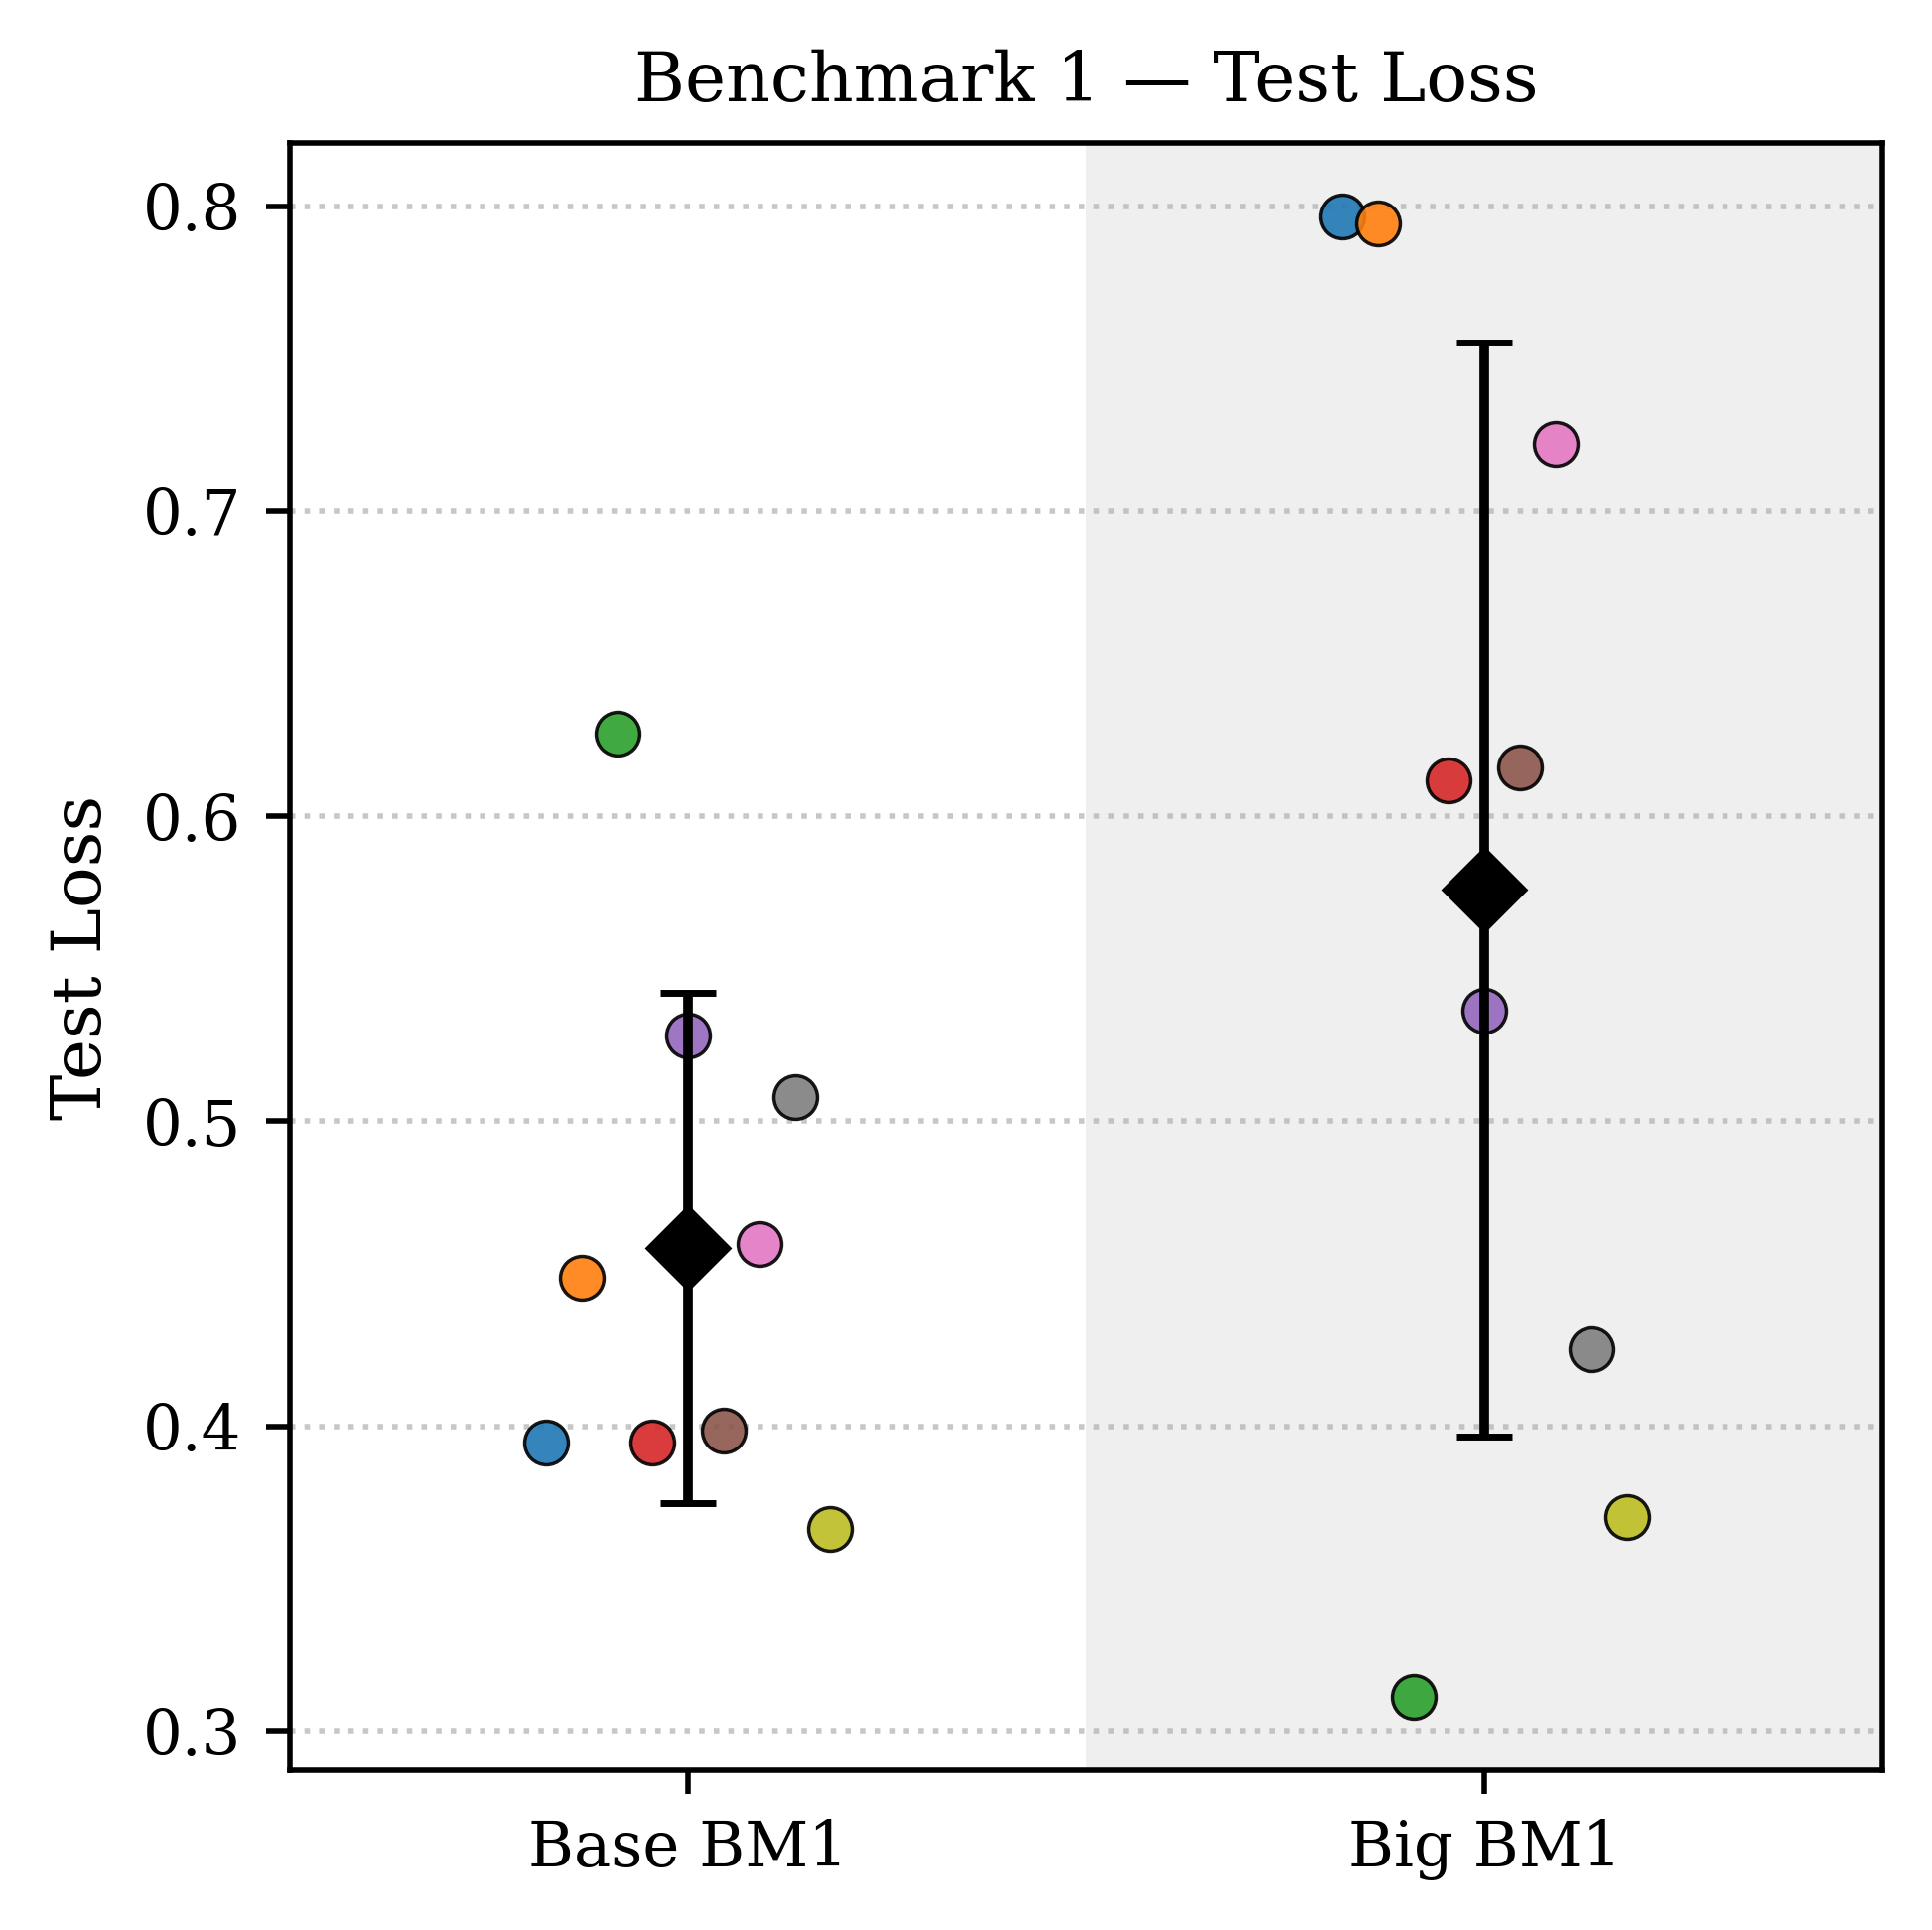
\includegraphics[width=0.9\textwidth]{chapters/7-results_and_discussion/bm1/bm1_test_loss.png}
        \caption{}
    \end{subfigure}
    \caption{Benchmark 1 results. (a) Test balanced accuracy with direct comparison of the Base config consisting of the \texttt{Base} PatchTST model on \texttt{FT} only and the Big config with the \texttt{Big} PatchTST model on the best channels.}
    \label{fig:bm1_test_result}
\end{figure}

\begin{table}[htbp]
    \centering
    \caption{Test balanced accuracy detailed results of Benchmark 1.}
    \label{tab:bm1_bal_acc_detail}
    \begin{tabular}{llll}
        \toprule
        \textbf{Domain} & \textbf{Mean $\pm$ std} & \textbf{Min (ms, ss)} & \textbf{Max (ms, ss)}\\
        \midrule

        \texttt{Base BM1} & 0.8617 $\pm$ 0.0130 & 0.8410 (420, 42) & 0.8768 (42, 69)\\
        \texttt{Big BM1} & 0.8909 $\pm$ 0.0066 & 0.8816 (420, 420) & 0.9004 (420, 69) \\
        \bottomrule
    \end{tabular}
\end{table}

\begin{table}[htbp]
    \centering
    \caption{Exact Train, Validation, Test splits with class balance for Benchmark 1.}
    \label{tab:bm1_data_split}
    \begin{tabular}{lll}
        \toprule
        \textbf{Training (pos, neg)} & \textbf{Validation (pos, neg)} & \textbf{Test (pos, neg)}\\
        \midrule

        5852 (3173, 2679) & 1033 (560, 473) & 1215 (659, 556)\\
        \bottomrule
    \end{tabular}
\end{table}
\newpage

% MARK: BM2
\section{Benchmark 2: Test on Individual Hole}
\label{sec:results_benchmark2}

Benchmark 2 evaluates the model on individual held-out hole domains. In contrast to Benchmark 1, the test samples are not drawn from a mixed split over the same overall distribution, but from one complete hole domain, containing each a unique rod type and tolerance level, that is excluded from training and validation data. The benchmark therefore tests whether the model can transfer the learned classification behavior to a hole domain that was not observed during training. The exact train, validation, and test splits are listed in \tabref{tab:bm2_data_split}. Each held-out domain contains either 820 ($820 = 100 + 360 + 360$) or 1060 ($1060 = 100 + 480 + 480$) test samples, with both classes represented.

\begin{figure}[htbp]
    \centering
    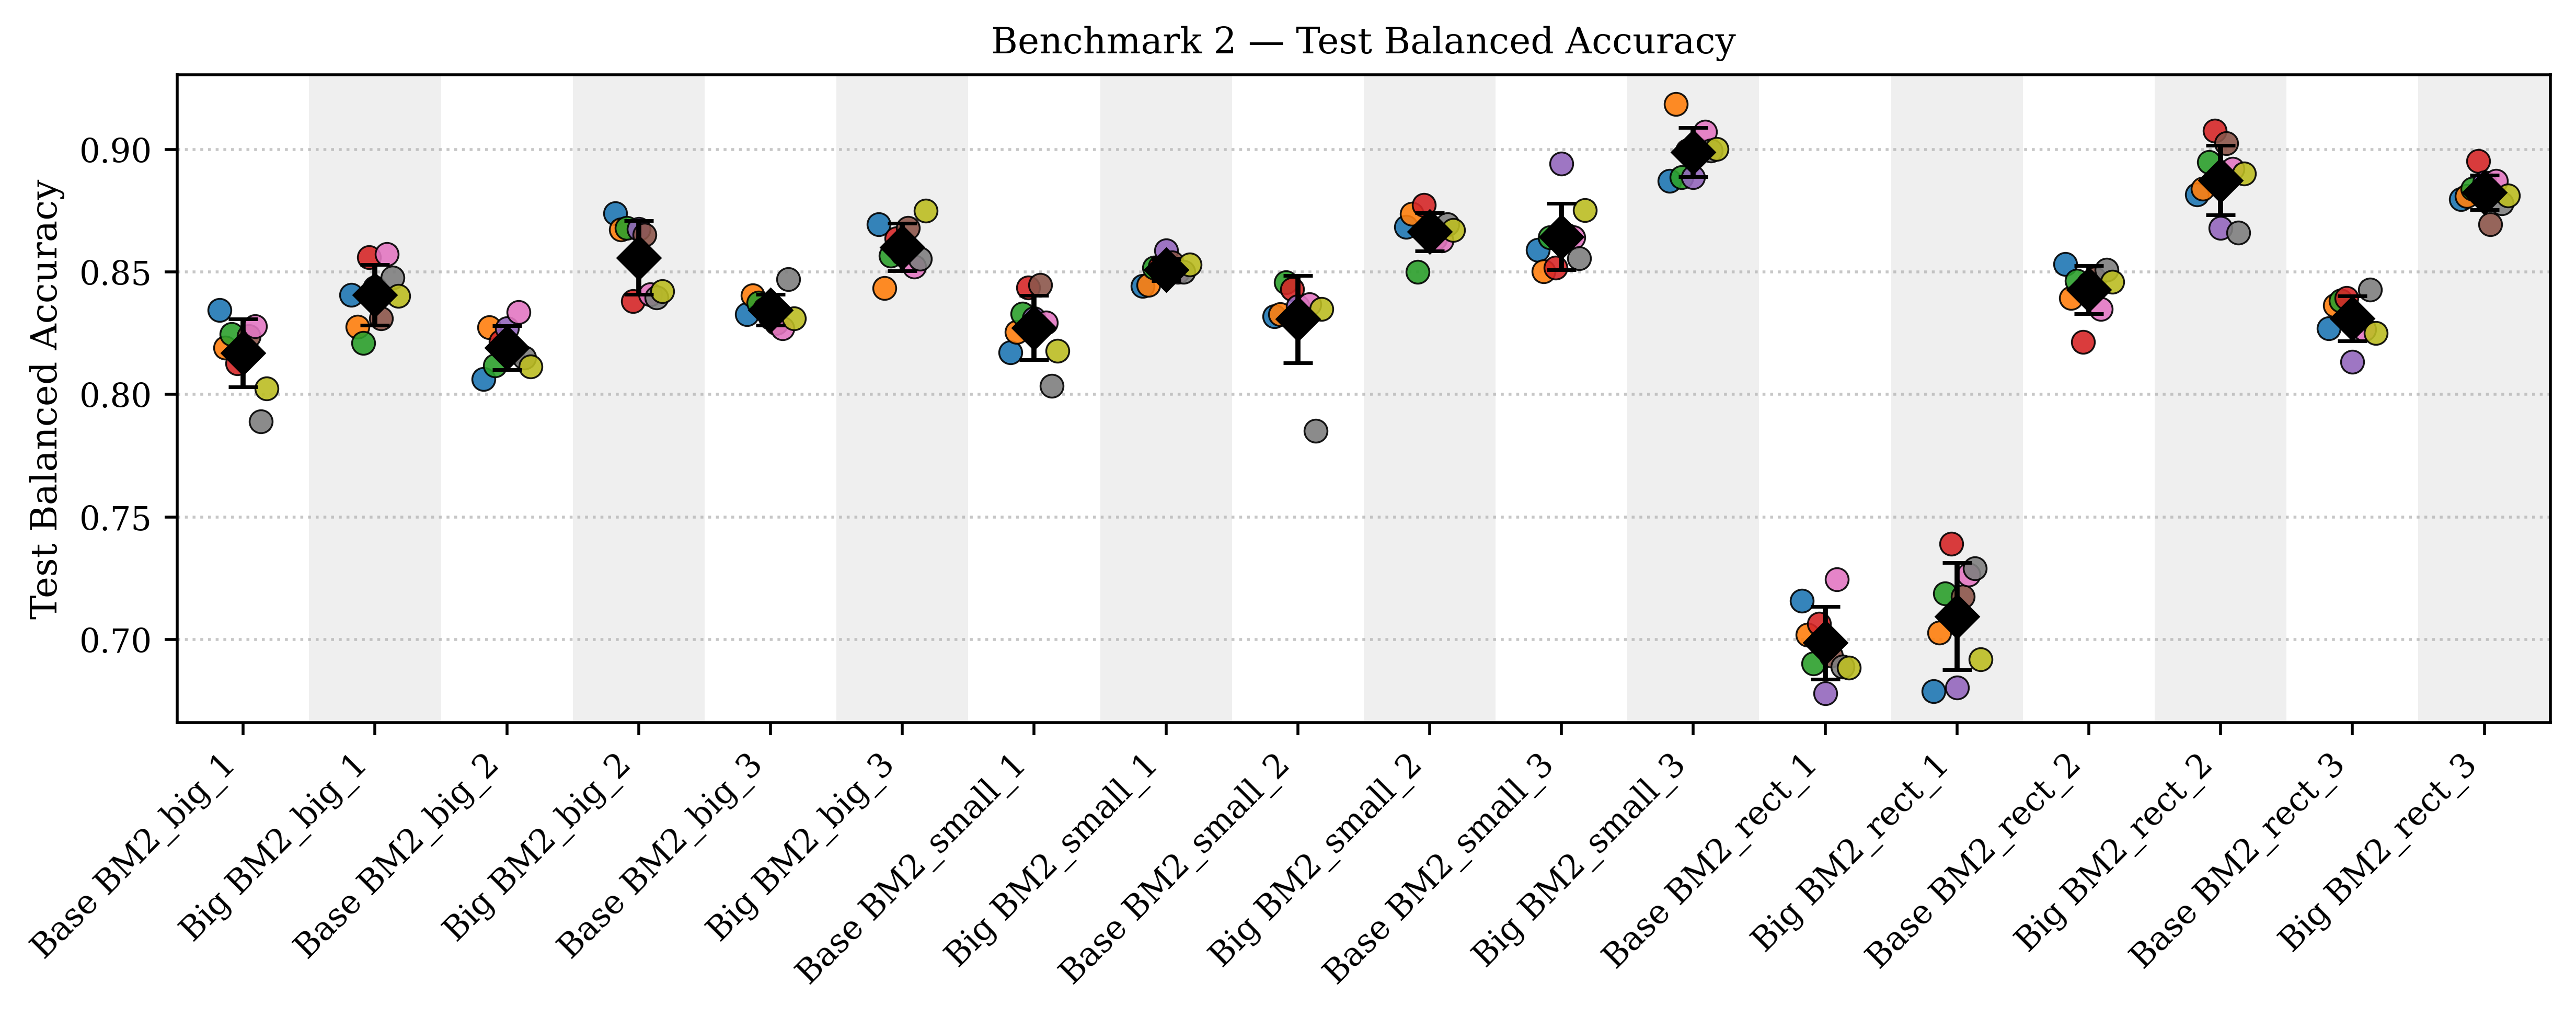
\includegraphics[width=1.0\linewidth]{chapters/7-results_and_discussion/bm2/bm2_test_bal_acc.png}
    \caption{Test balanced accuracy of all of all hole domains specified in \tabref{tab:bm2_domains} evaluated on both the Base and Big config.}
    \label{fig:bm2_test_bal_acc_result}
\end{figure}

\begin{figure}[htbp]
    \centering
    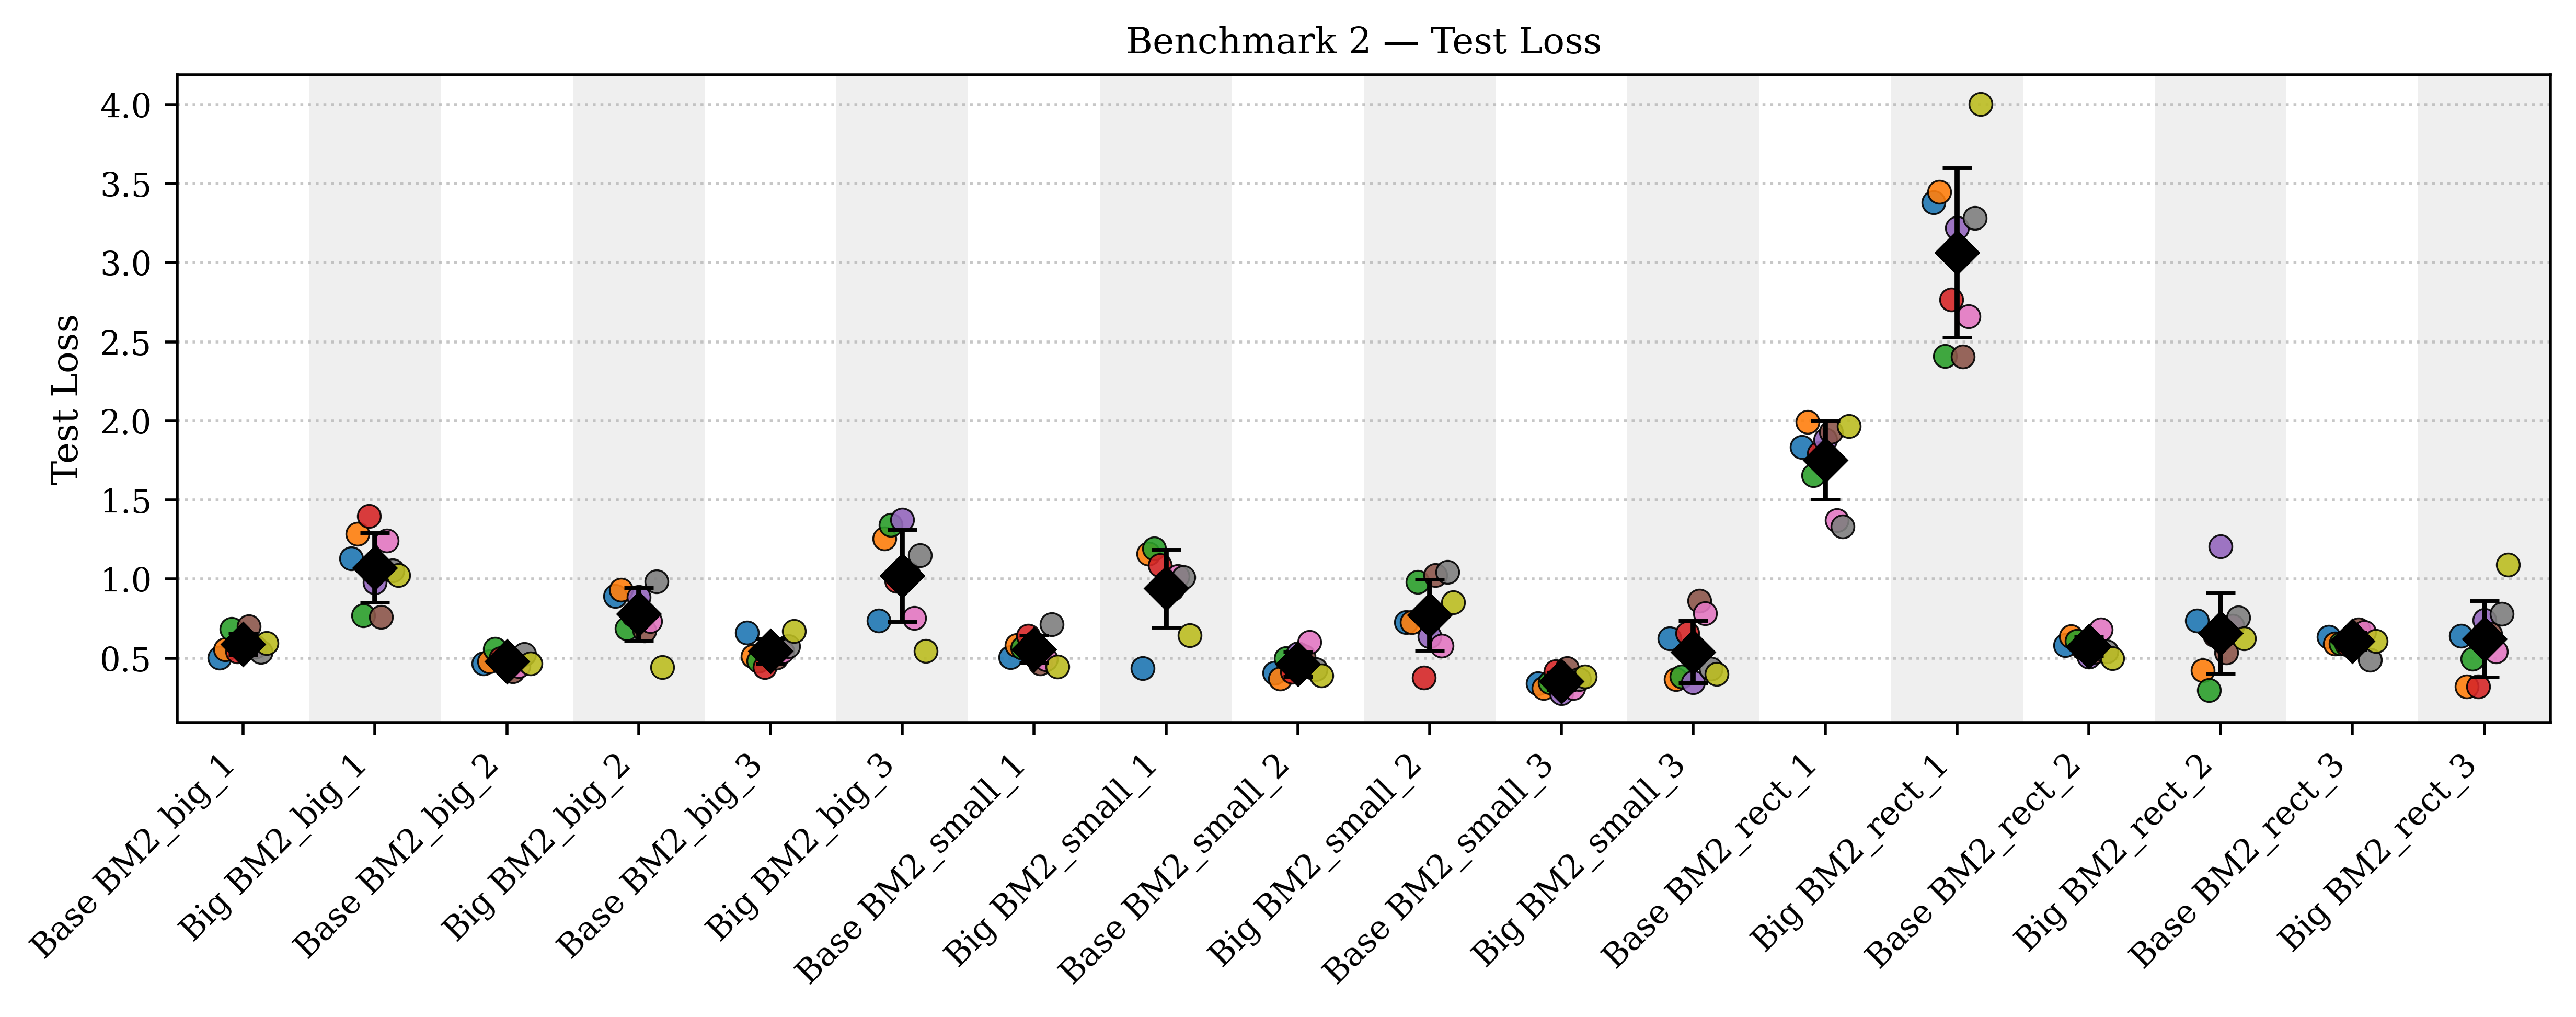
\includegraphics[width=1.0\linewidth]{chapters/7-results_and_discussion/bm2/bm2_test_loss.png}
    \caption{Test loss of all of all hole domains specified in \tabref{tab:bm2_domains} evaluated on both the Base and Big config.}
    \label{fig:bm2_test_loss_result}
\end{figure}

The detailed TBA values are reported in \tabref{tab:bm2_bal_acc_detail} and visualized in \figref{fig:bm2_test_bal_acc_result}. Both configs reach balanced accuracies above 0.80 for most held-out domains. The Big config achieves a higher mean balanced accuracy than the Base config in all evaluated domains. This shows that the increased model capacity in combination with the selected best channel inputs, is not only beneficial in the mixed split of Benchmark 1, but also improves classification performance to unseen individual hole domains. However, the improvement is not equally strong for all domains. For most domains, the Big config improves the mean TBA by roughly 0.02 to 0.05 points, while the improvement for \texttt{BM2\_rect\_1} is much smaller.

The best results are obtained for \texttt{BM2\_small\_3}, \texttt{BM2\_rect\_2}, and \texttt{BM2\_rect\_3}. In these domains, the Big config reaches mean TBA's close to or above 0.88, with \texttt{BM2\_small\_3} reaching the highest value of 0.8988. These results indicate that several individual hole domains can be classified reliably even when they are completely excluded from the training data. Therefore, the model does not only memorize individual hole conditions, but learns valuable patterns that prove to be useful under moderate domain shifts.

The clear exception is \texttt{BM2\_rect\_1}. Both configs perform much worse on this domain than on all other held-out domains, with mean TBA's of 0.6986 for the Base config and 0.7094 for the Big config. \texttt{BM2\_rect\_1} appears to represent a domain-specific shift in which the success and failure patterns are much more different from the remaining domains used for training and validation. The class balance of the test set is also balanced, differing by only 18 samples, so the reduced performance cannot be explained by an unbalanced class distribution alone.

A broader trend across the held-out domains is that tighter tolerances reduce the TBA. This can be seen for all rod types, where the first tolerance level generally leads to lower balanced accuracy than the looser tolerance levels. However, this effect is not equally strong for all geometries. For the round hole cases, represented by the \texttt{big} and \texttt{small} rod domains, the tighter tolerance of corresponding holes reduces performance but much more gradually than for rectangular holes. In fact, the tightest tolerance of the rectangular holes, \texttt{BM2\_rect\_1}, behaves fundamentally differently from \texttt{BM2\_rect\_2} and \texttt{BM2\_rect\_3}. This indicates that tight tolerances in rectangular holes generate signal patterns that differ much more from the remaining tolerance levels than tight tolerances in round holes. The rectangular geometry therefore appears to create a more severe domain shift when combined with the tightest tolerance. In addition, the \texttt{small} rod domains are generally easier to classify than the \texttt{big} rod domains, with especially good performance for \texttt{BM2\_small\_3}.

The test loss values in \figref{fig:bm2_test_loss_result} support the interpretation of \texttt{BM2\_rect\_1} as the most difficult held-out domain. It shows the highest loss values and the largest spread across seeds, especially for the Big config. However, the loss does not show the same consistent tolerance-dependent trend as the balanced accuracy does. This indicates that tighter tolerances mainly reduce the final classification performance, while the loss is more affected by individual difficult domains and by the confidence of wrong predictions.

Overall, Benchmark 2 shows that the model can generalize to most individual unseen hole domains with good test balanced accuracy. The Big config is preferable when classification performance is evaluated by balanced accuracy, because it improves the mean predictions in every domain. However, the results also show that generalization is very much domain-dependent. Tighter tolerances generally reduce balanced accuracy, but this effect is much more visible for rectangular holes than for round holes. The tightest rectangular domain, \texttt{BM2\_rect\_1}, therefore reveals a clear limitation of generalization and indicates that some combinations of geometry and tolerance introduce much stronger domain shifts than others. Benchmark 2 therefore provides a more realistic reference than Benchmark 1 and motivates the group-level generalization analysis in Benchmark 3.


\begin{table}[htbp]
    \centering
    \caption{Test balanced accuracy detailed results of Benchmark 2. Rows in bold show the highest test balanced accuracy, while underlined rows show the lowest test balanced accuracy.}
    \label{tab:bm2_bal_acc_detail}
    \begin{tabular}{llll}
        \toprule
        \textbf{Domain} & \textbf{Mean $\pm$ std} & \textbf{Min (ms, ss)} & \textbf{Max (ms, ss)}\\
        \midrule 

        \texttt{Base BM2\_big\_1} & \underline{0.8169} $\pm$ \underline{0.0139} & \underline{0.7889 (420, 69)} & \underline{0.8344 (42, 42)}\\
        \texttt{Big BM2\_big\_1} & 0.8406 $\pm$ 0.0124 & 0.8209 (42, 420) & 0.8573 (420, 42) \\
        \texttt{Base BM2\_big\_2} & 0.8190 $\pm$ 0.0090 & 0.8062 (42, 42) & 0.8336 (420, 42)\\
        \texttt{Big BM2\_big\_2} & 0.8558 $\pm$ 0.0151 & 0.8381 (69, 42) & 0.8739 (42, 42) \\
        \texttt{Base BM2\_big\_3} & 0.8345 $\pm$ 0.0062 & 0.8270 (420, 42) & 0.8469 (420, 69)\\
        \texttt{Big BM2\_big\_3} & 0.8601 $\pm$ 0.0097 & 0.8435 (42, 69) & 0.8749 (420, 420) \\
        \midrule
        \texttt{Base BM2\_small\_1} & 0.8272 $\pm$ 0.0131 & 0.8034 (420, 69) & 0.8446 (69, 420)\\
        \texttt{Big BM2\_small\_1} & 0.8509 $\pm$ 0.004 & 0.8442 (42, 42) & 0.8588 (69, 69) \\
        \texttt{Base BM2\_small\_2} & 0.8308 $\pm$ 0.0178 & 0.7850 (420, 69) & 0.8458 (42, 420)\\
        \texttt{Big BM2\_small\_2} & 0.8664 $\pm$ 0.0077 & 0.8499 (42, 420) & 0.8774 (69, 42) \\
        \texttt{Base BM2\_small\_3} & 0.8643 $\pm$ 0.0136 & 0.8502 (42, 69) & 0.8942 (69, 69)\\
        \texttt{Big BM2\_small\_3} & \textbf{0.8988} $\pm$ \textbf{0.0100} & \textbf{0.8872 (42, 42)} & \textbf{0.9184 (42, 69)} \\
        \midrule
        \texttt{Base BM2\_rect\_1} & \underline{0.6986} $\pm$ \underline{0.0148} & \underline{0.6779 (69, 69)} & \underline{0.7246 (420, 42)}\\
        \texttt{Big BM2\_rect\_1} & 0.7094 $\pm$ 0.0219 & 0.6789 (42, 42) & 0.7391 (69, 42) \\
        \texttt{Base BM2\_rect\_2} & 0.8427 $\pm$ 0.0097 & 0.8214 (69, 42) & 0.8532 (42, 42)\\
        \texttt{Big BM2\_rect\_2} & \textbf{0.8874} $\pm$ \textbf{0.0141} & \textbf{0.8661 (420, 69)} & \textbf{0.9076 (69, 42)} \\
        \texttt{Base BM2\_rect\_3} & 0.8310 $\pm$ 0.0092 & 0.8132 (69, 69) & 0.8427 (420, 69)\\
        \texttt{Big BM2\_rect\_3} & \textbf{0.8824} $\pm$ \textbf{0.0071} & \textbf{0.8695 (69, 420)} & \textbf{0.8951 (69, 42)} \\
        \bottomrule
    \end{tabular}
\end{table}

\begin{table}[htbp]
    \centering
    \caption{Exact Train, Validation, Test splits with class balance for Benchmark 2.}
    \label{tab:bm2_data_split}
    \begin{tabular}{llll}
        \toprule
        \textbf{Domain} & \textbf{Training (pos, neg)} & \textbf{Validation (pos, neg)} & \textbf{Test (pos, neg)}\\
        \midrule

        \texttt{BM2\_big\_1} & 5984 (3254, 2730) & 1056 (574, 482) & 1060 (564, 496)\\
        \texttt{BM2\_big\_2} & 6188 (3350, 2838) & 1092 (591, 501) & 820 (451, 369)\\
        \texttt{BM2\_big\_3} & 6188 (3365, 2823) & 1092 (594, 498) &  820 (433, 387)\\
        
        \texttt{BM2\_small\_1} & 5984 (3199, 2785) & 1056 (565, 491) & 1060 (628, 432)\\
        \texttt{BM2\_small\_2} & 6188 (3296, 2892) & 1092 (582, 510) & 820 (514, 306)\\
        \texttt{BM2\_small\_3} & 6188 (3397, 2791) & 1092 (600, 492) & 820 (395, 425)\\

        \texttt{BM2\_rect\_1} & 5984 (3290, 2694) & 1056 (581, 475) & 1060 (521, 539)\\
        \texttt{BM2\_rect\_2} & 6188 (3343, 2845) & 1092 (590, 502) & 820 (459, 361)\\
        \texttt{BM2\_rect\_3} & 6188 (3370, 2818) & 1092 (595, 497) & 820 (427, 393)\\
        \bottomrule
    \end{tabular}
\end{table}

\newpage

% MARK: BM3
\section{Benchmark 3: Test on Held-Out Group}
\label{sec:results_benchmark3}

Benchmark 3 evaluates generalization to held-out domain groups. The held-out groups correspond to complete batches, rod types, tolerance levels, or gripper types. The exact train, validation, and test splits are listed in \tabref{tab:bm3_data_split}. Depending on the held-out domain, the test sets contain between 900 and 3600 samples, and being balanced more unevenly, with however bigger classes over all than for Benchmark 2. The biggest class imbalance has the \texttt{BM3\_tol\_2} class with a difference of 388 samples. The detailed test balanced accuracy results are reported in \tabref{tab:bm3_bal_acc_detail}.

\begin{figure}[htbp]
    \centering
    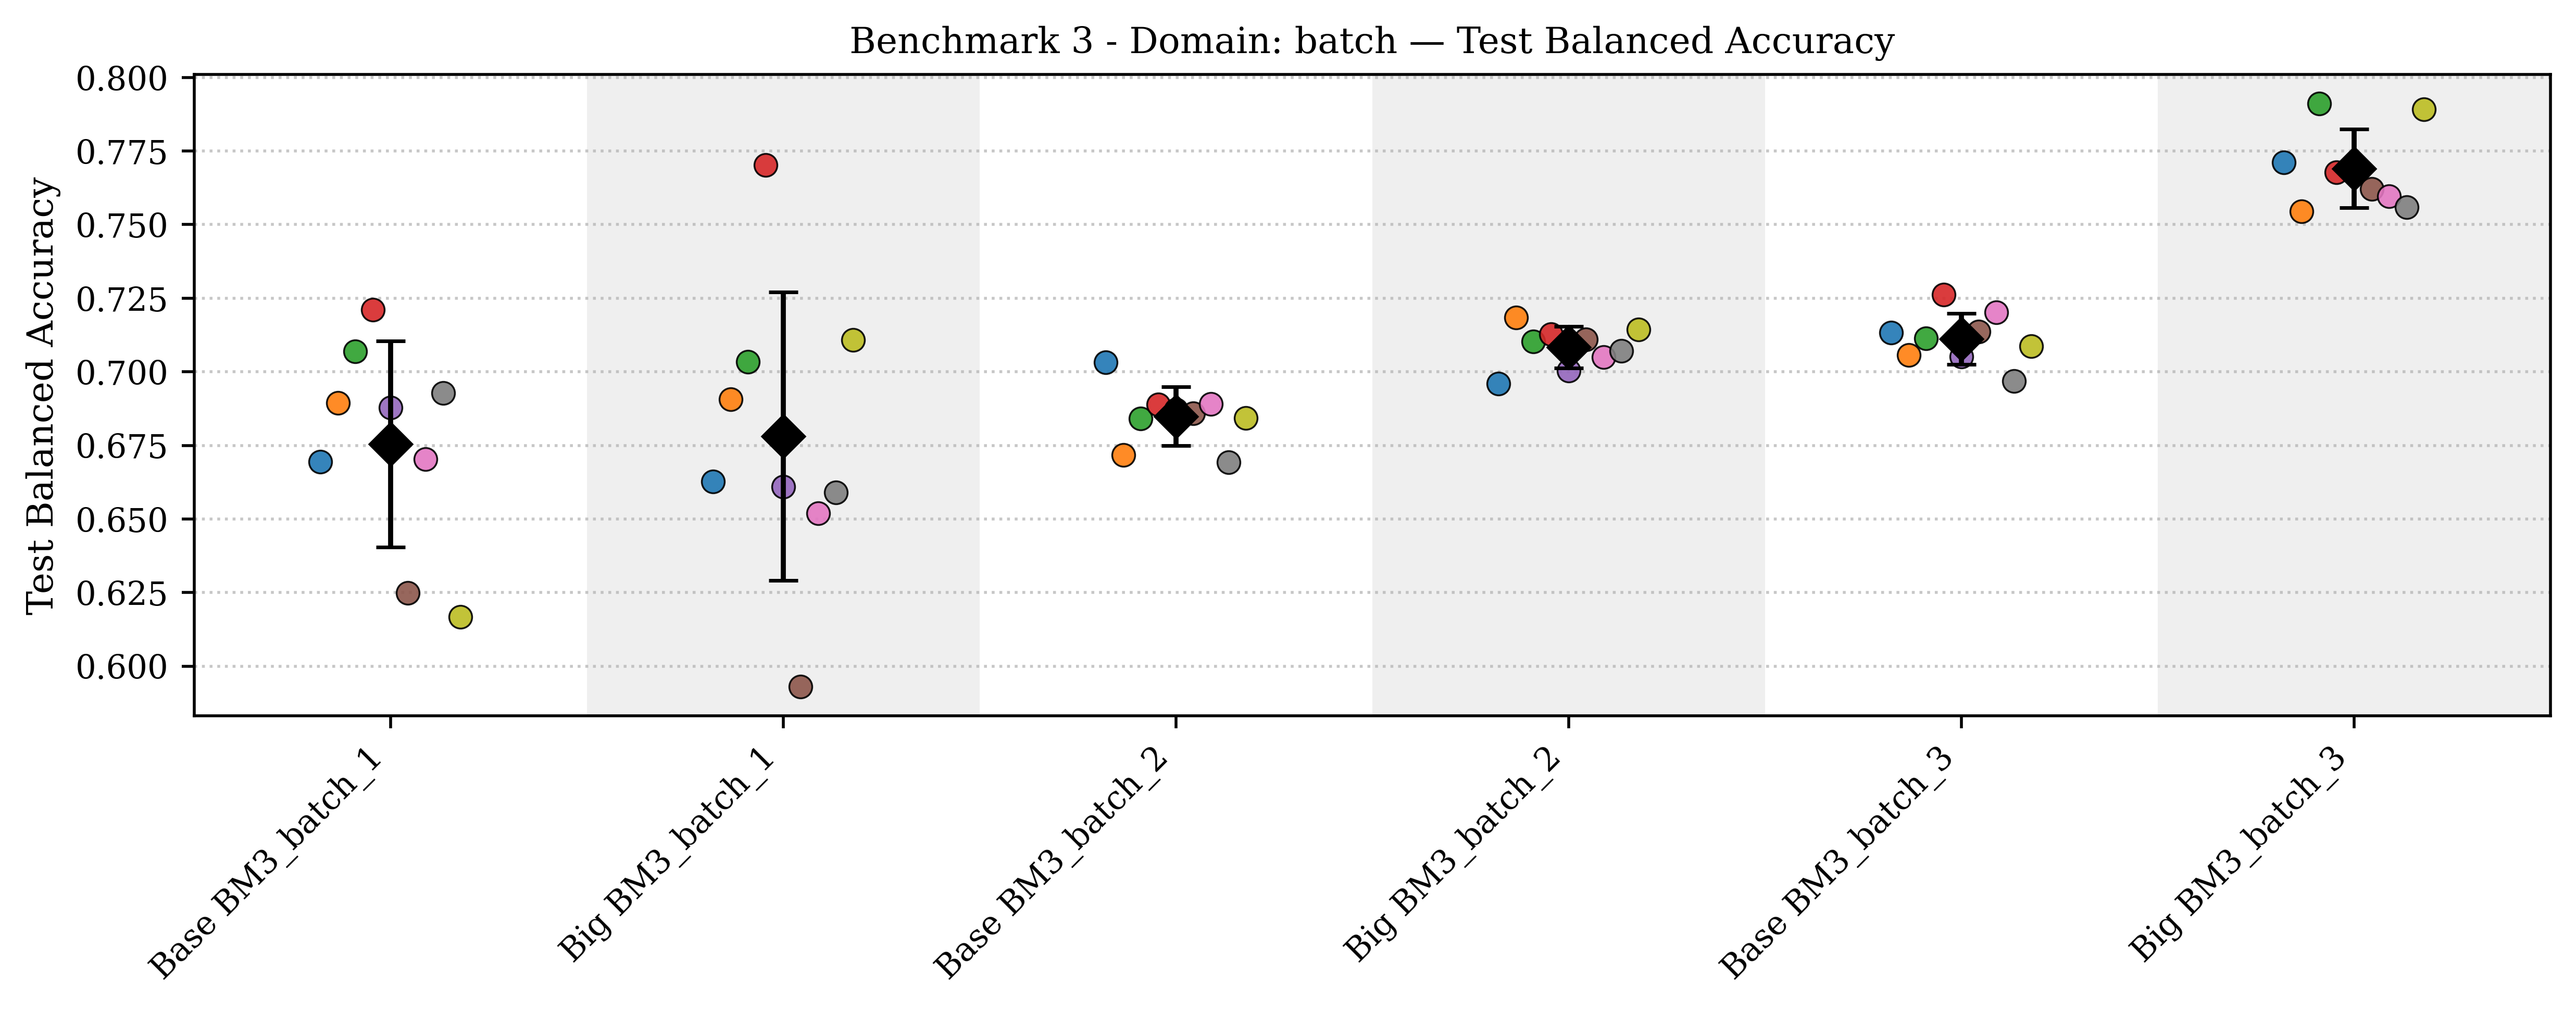
\includegraphics[width=1.0\linewidth]{chapters/7-results_and_discussion/bm3/bm3_batch_test_bal_acc.png}
    \caption{Test balanced accuracy of the held-out batch domains, evaluated with the Base and Big config. Colored points show the individual seed combinations, while the black markers show the mean and standard deviation.}
    \label{fig:bm3_batch_test_bal_acc}
\end{figure}

\begin{figure}[htbp]
    \centering
    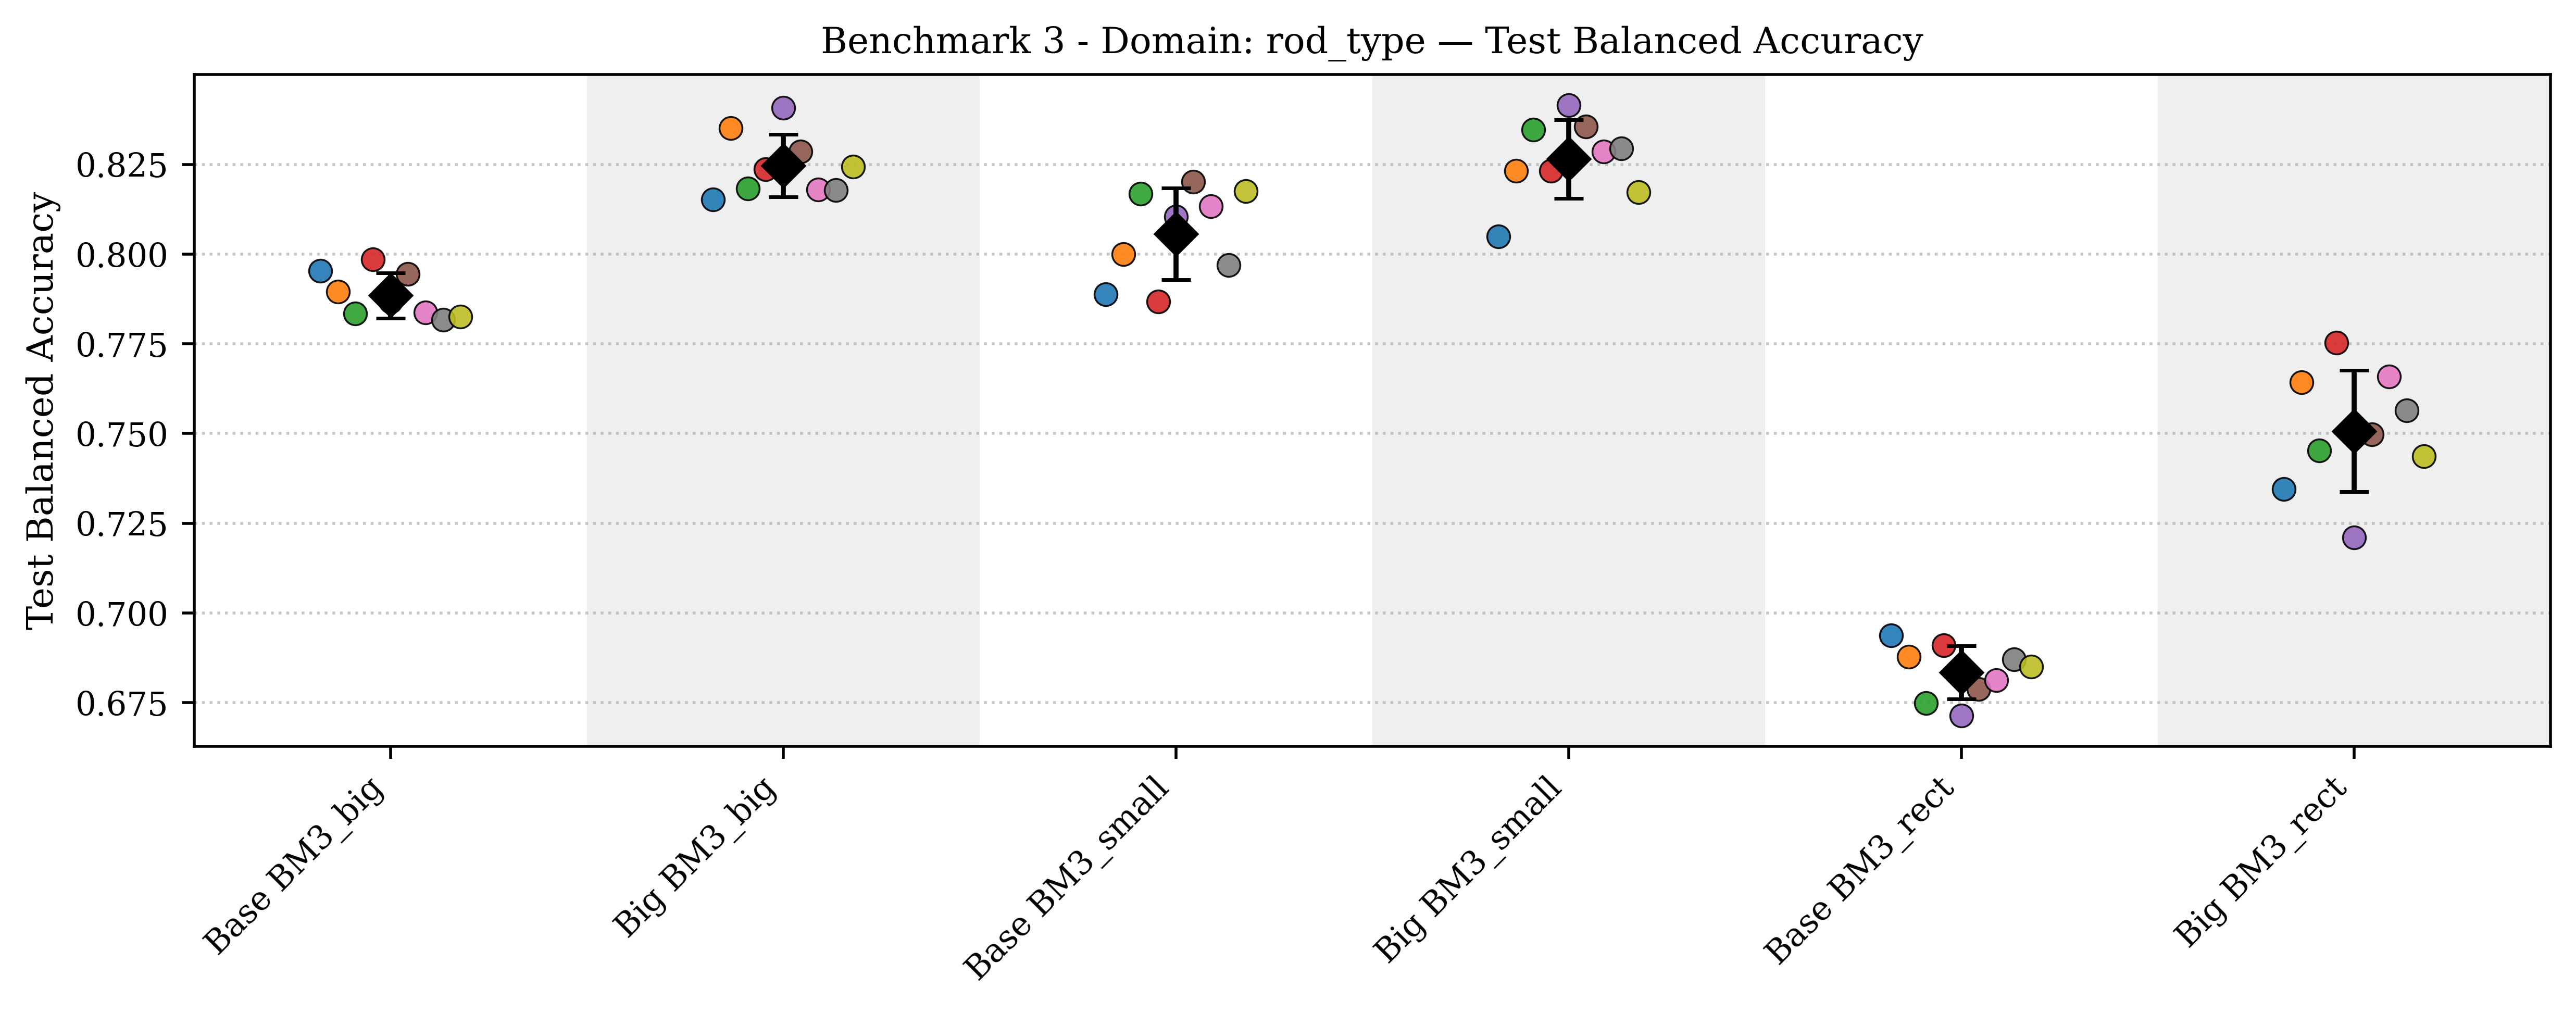
\includegraphics[width=1.0\linewidth]{chapters/7-results_and_discussion/bm3/bm3_rod_type_test_bal_acc.png}
    \caption{Test balanced accuracy of the held-out rod-type domains, evaluated with the Base and Big config. Colored points show the individual seed combinations, while the black markers show the mean and standard deviation.}
    \label{fig:bm3_rod_type_test_bal_acc}
\end{figure}

\begin{figure}[htbp]
    \centering
    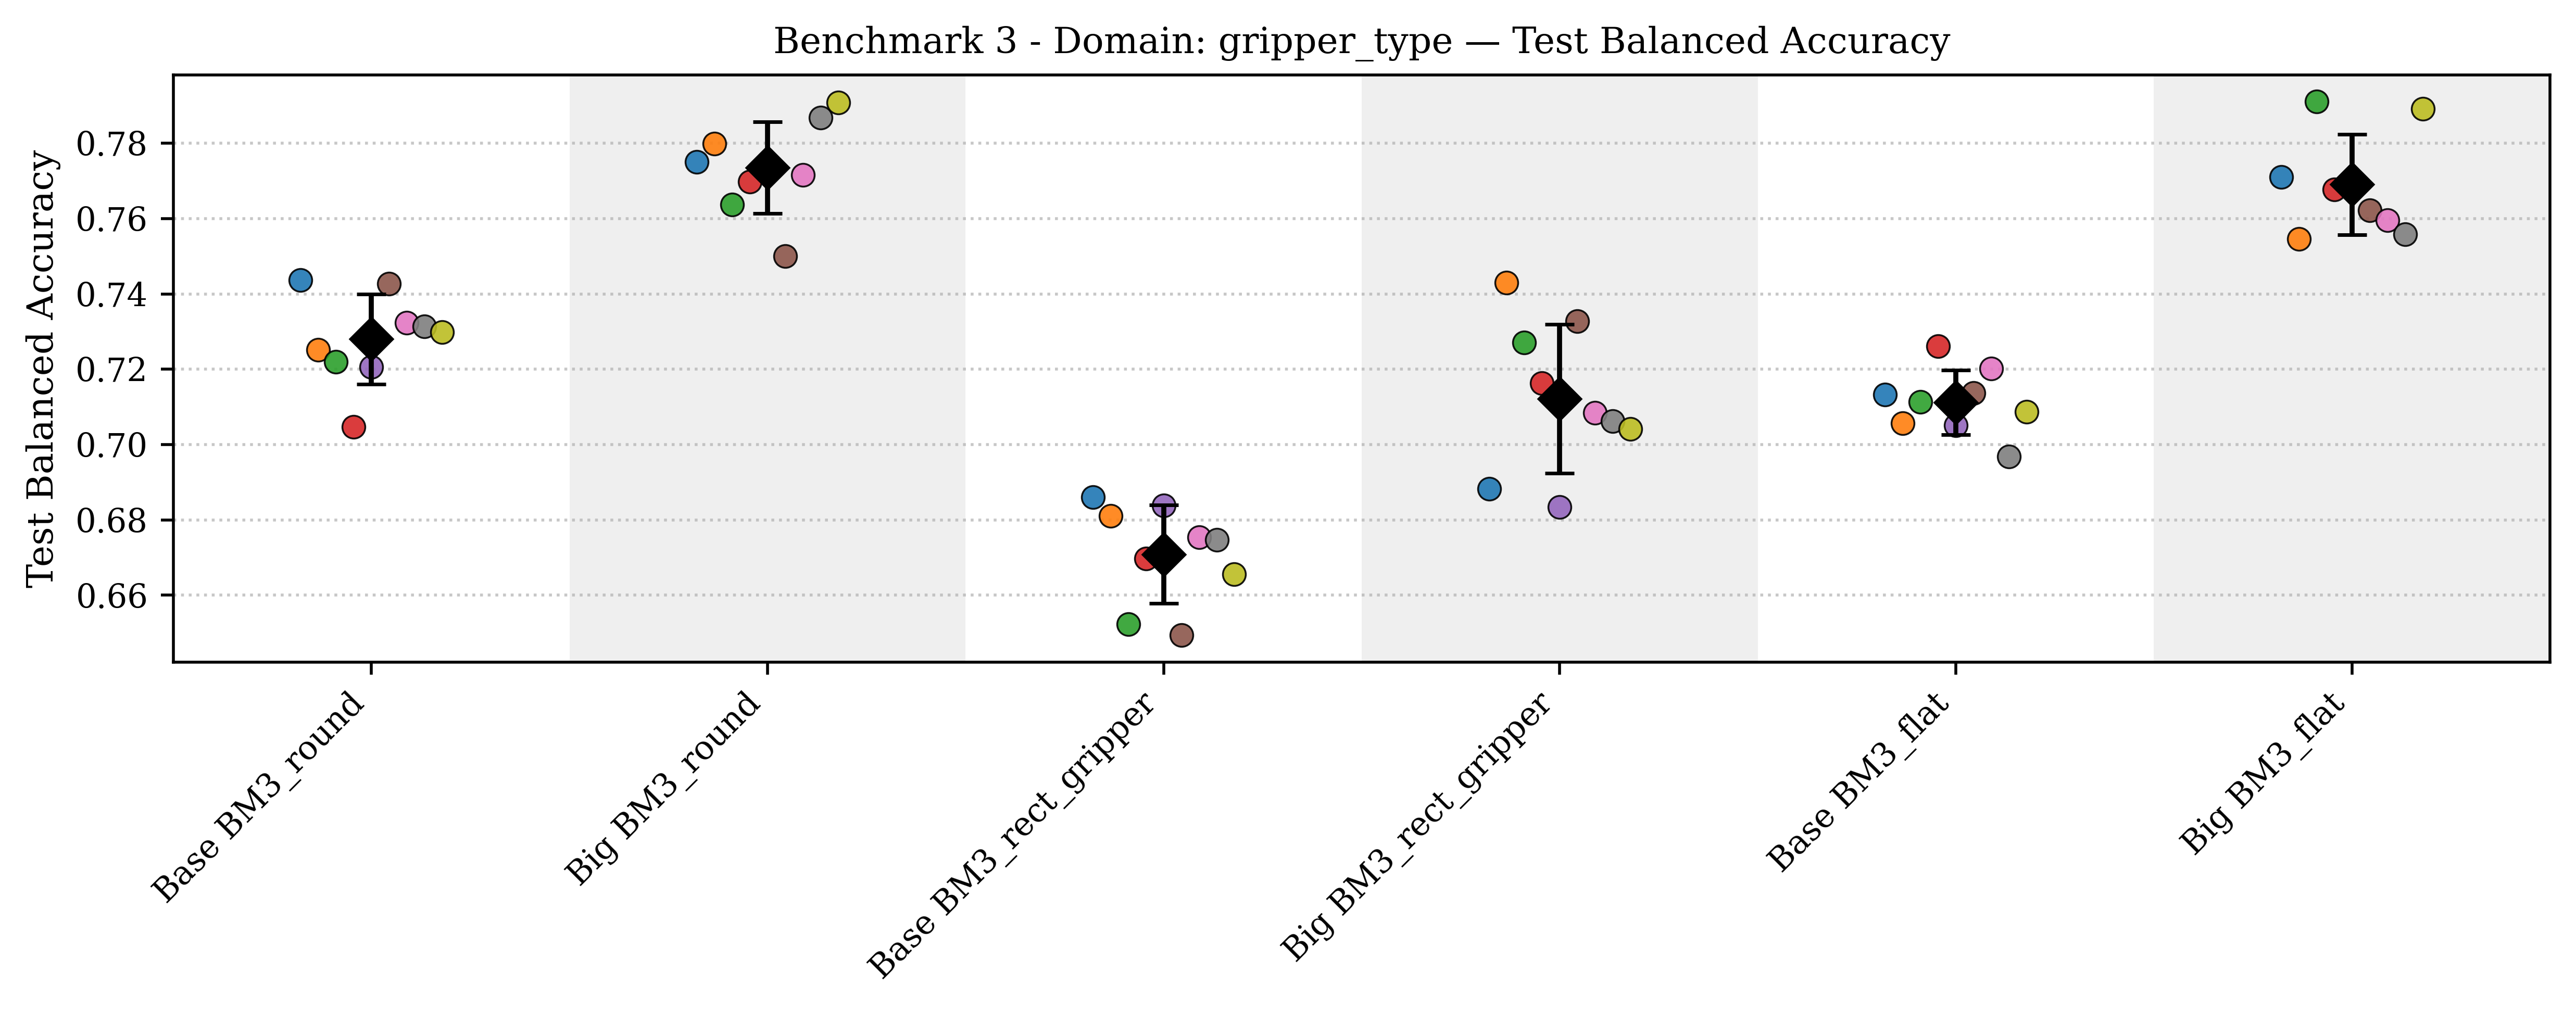
\includegraphics[width=1.0\linewidth]{chapters/7-results_and_discussion/bm3/bm3_gripper_type_test_bal_acc.png}
    \caption{Test balanced accuracy of the held-out gripper-type domains, evaluated with the Base and Big config. Colored points show the individual seed combinations, while the black markers show the mean and standard deviation.}
    \label{fig:bm3_gripper_type_test_bal_acc}
\end{figure}

\begin{figure}[htbp]
    \centering
    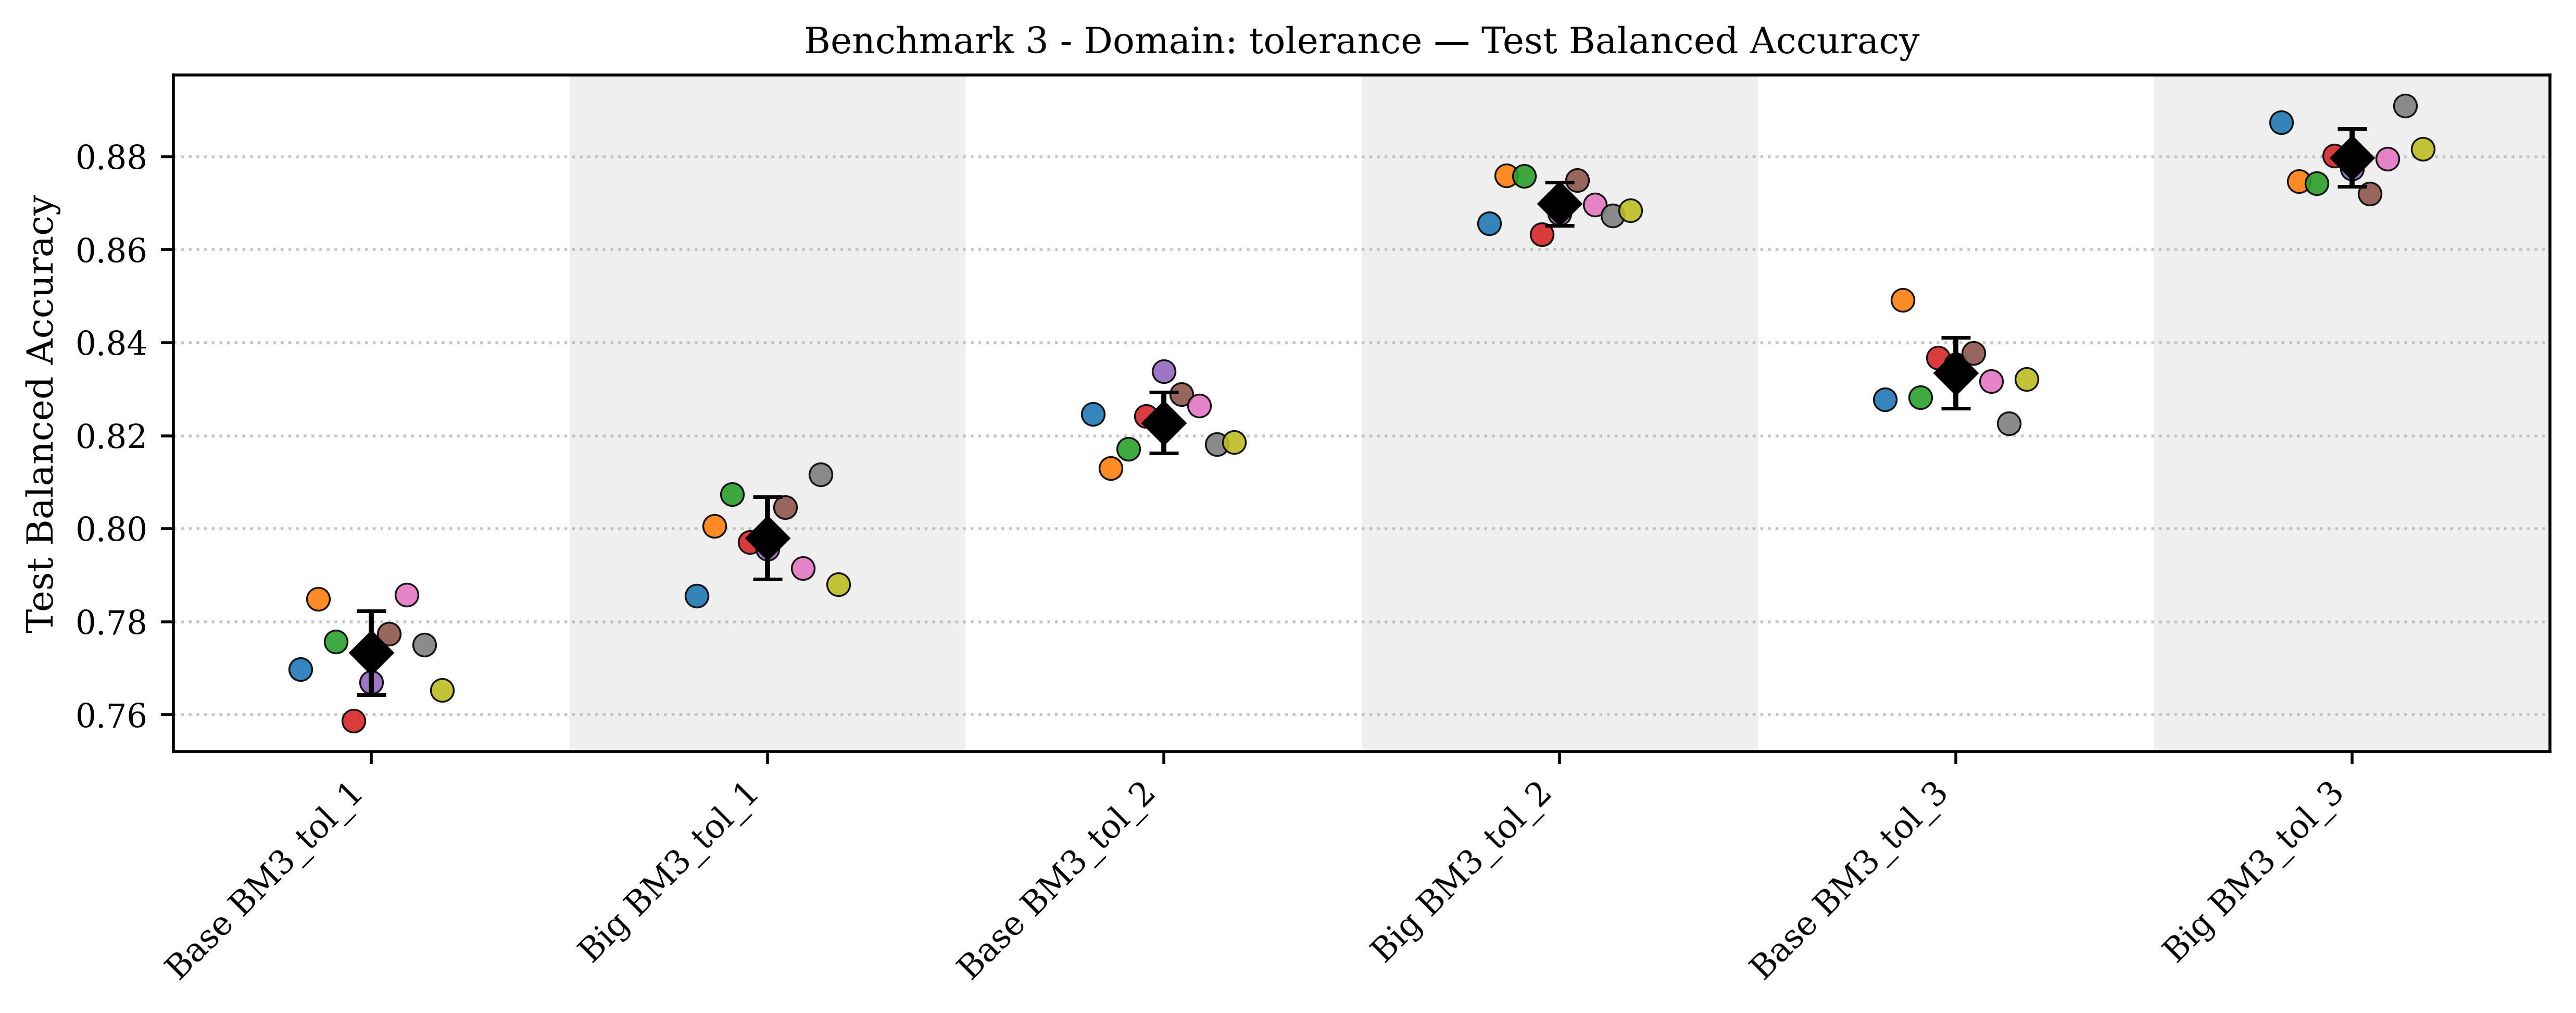
\includegraphics[width=1.0\linewidth]{chapters/7-results_and_discussion/bm3/bm3_tolerance_test_bal_acc.png}
    \caption{Test balanced accuracy of the held-out tolerance domains, evaluated with the Base and Big config. Colored points show the individual seed combinations, while the black markers show the mean and standard deviation.}
    \label{fig:bm3_tolerance_test_bal_acc}
\end{figure}

\begin{figure}[htbp]
    \centering
    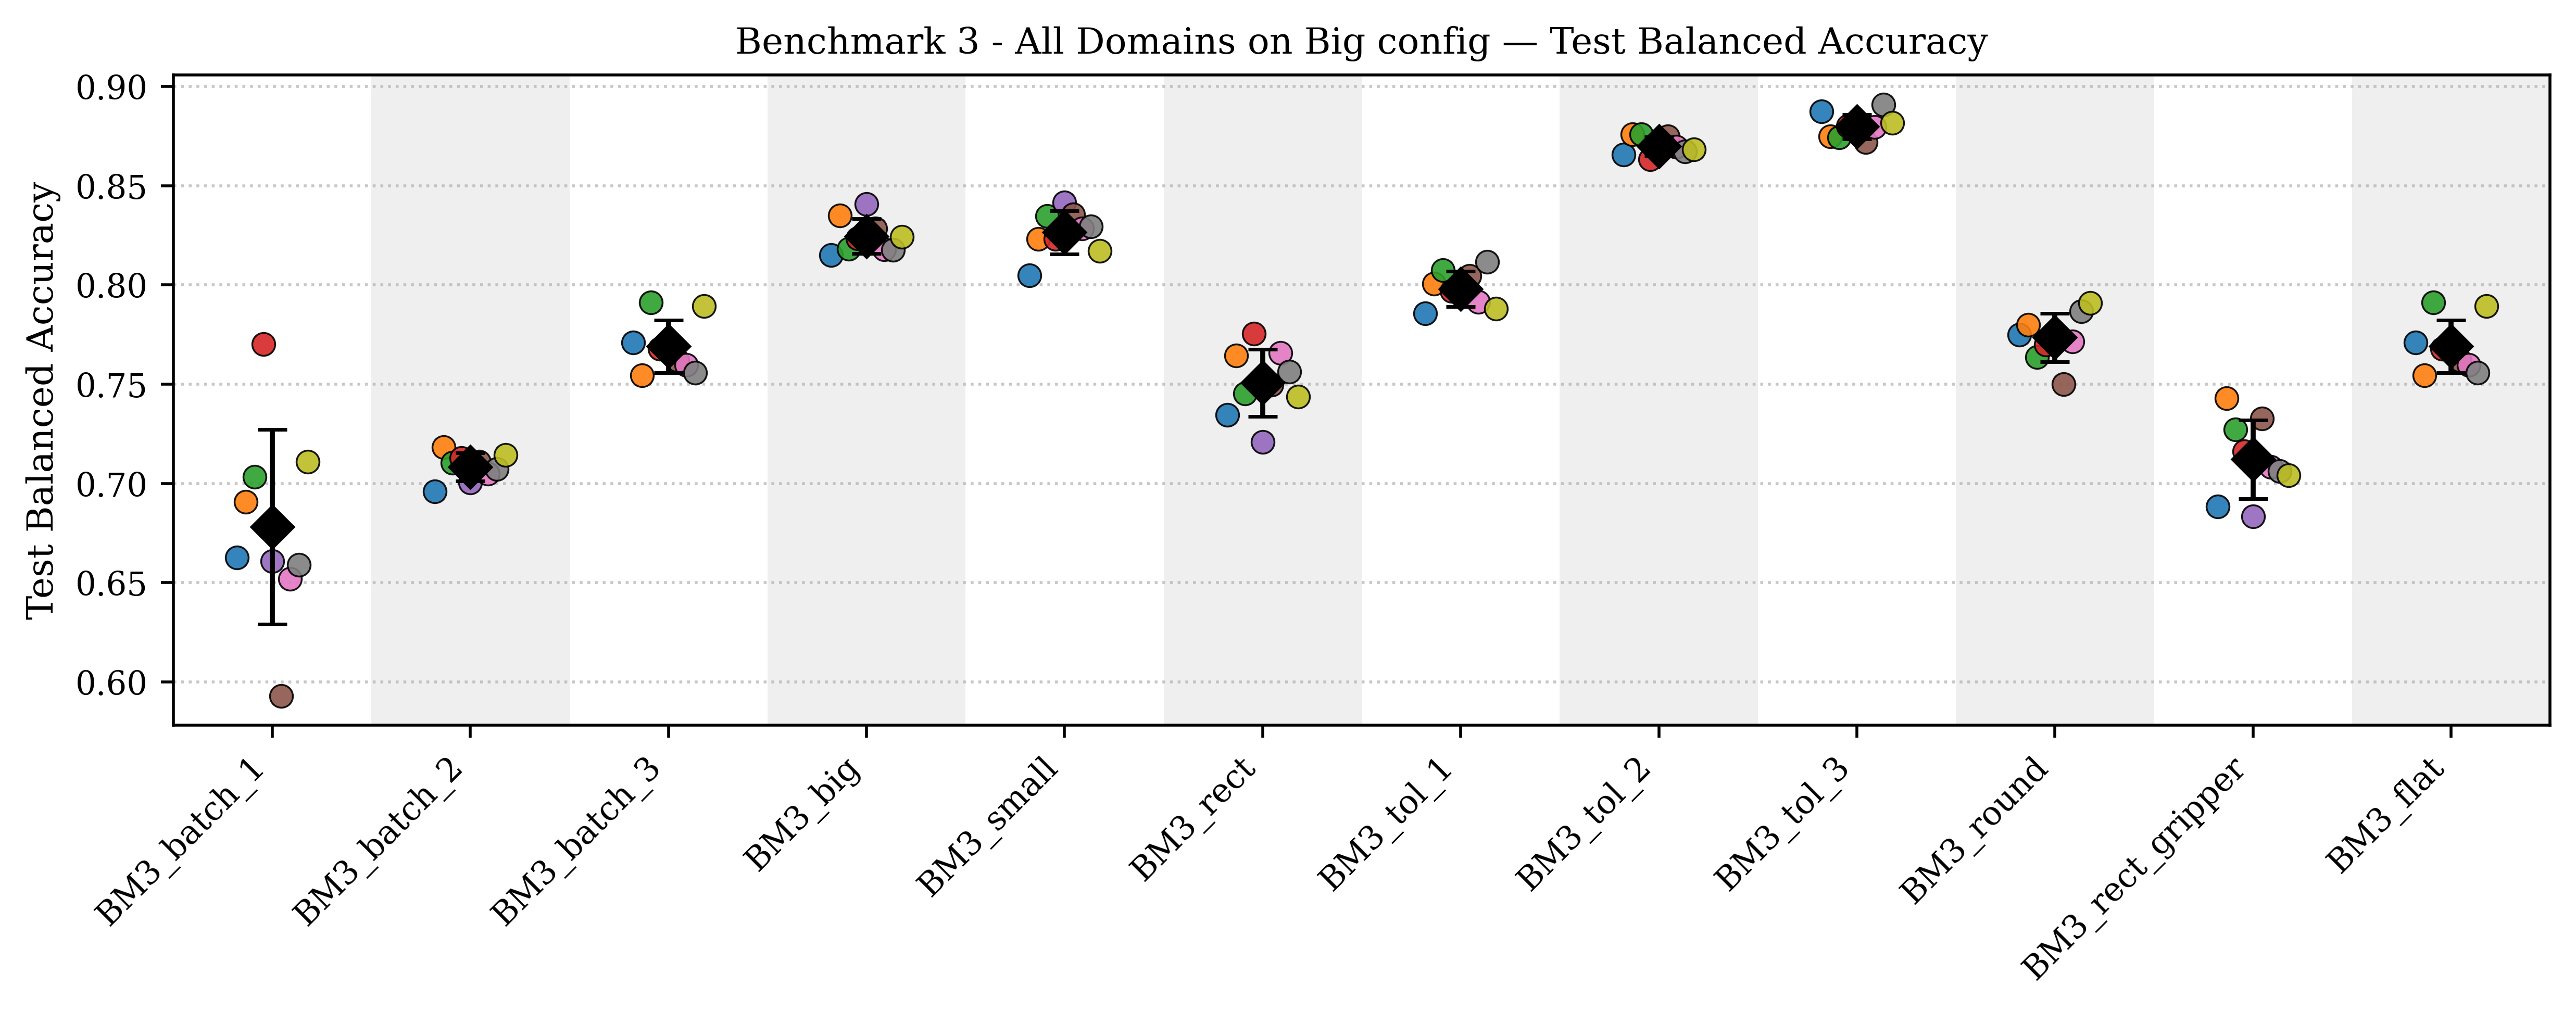
\includegraphics[width=1.0\linewidth]{chapters/7-results_and_discussion/bm3/bm3_all_domains_test_bal_acc.png}
    \caption{Summary of the Big config test balanced accuracy across all held-out domain groups in Benchmark 3. Colored points show the individual seed combinations, while the black markers show the mean and standard deviation.}
    \label{fig:bm3_all_domains_test_bal_acc}
\end{figure}

The results for the held-out \texttt{batch} domains are shown in \figref{fig:bm3_batch_test_bal_acc}. These domains produce some of the lowest test balanced accuracies in Benchmark 3. The Big config reaches mean balanced accuracies of 0.6781, 0.7083, and 0.7691 for \texttt{BM3\_batch\_1}, \texttt{BM3\_batch\_2}, and \texttt{BM3\_batch\_3}, respectively. The largest seed-dependent spread is observed for \texttt{BM3\_batch\_1}. This indicates that the batch split introduces a particularly difficult domain shift. In contrast to a single hole condition, a batch can contain several coupled changes, such as differences in execution, setup state, or sample composition. In particular, Batch 1 was recorded only with position offset and tilt, that got randomly sampled. Whereas in Batches 2 and 3 deviations got applied deterministically with six more deviation groups, instead of two. Also with entire batches being held-out as test data, the training data size becomes much smaller, which can cause overfitting to the training data that would result in worse test results. For held-out Batches 2 and 3 the training data size of each 3825 samples is the lowest in the entire benchmark, their mean balanced accuracies are higher than for batch 1. This contradiction could be explained due to the fact that batches 2 and 3 have the same deviation planner design, that produces more similar insertion conditions than compared to batch 1. The low balanced accuracies therefore suggest that the model is sensitive to batch-specific execution and deviation design that are not fully transferable across batches.

For the held-out \texttt{rod\_type} domains, the results in \figref{fig:bm3_rod_type_test_bal_acc} show that the Big config reaches similar performance for \texttt{BM3\_big} and \texttt{BM3\_small}, with mean balanced accuracies of 0.8246 and 0.8265. The small rod type is therefore at least as easy to classify as the big rod type, which is consistent with the results from Benchmark 2, where the small rod almost always scored slightly better than the big rod. In contrast, the held-out \texttt{BM3\_rect} domain is clearly harder, with a mean TBA of 0.7507 for the Big config. At the same time, the improvement of the Big config over the Base config is largest in the entire benchmark, with an increase of $0.7507 - 0.6834 = 0.0673$. This shows that the larger model makes use of the additional capacity and channels to improve classification of the rectangular rod domain, but it cannot fully close the gap to the round rod domains. The rectangular geometry therefore introduces a bigger change in the signal patterns than the difference between the big and small round rods.

The results for the held-out \texttt{gripper\_type} domains in \figref{fig:bm3_gripper_type_test_bal_acc} show mean TBAs of 0.7735 for \texttt{BM3\_round}, 0.7122 for \texttt{BM3\_rect\_gripper}, and 0.7691 for \texttt{BM3\_flat} with the Big config. The rectangular gripper condition is therefore the most difficult gripper-domain split. The Base config on \texttt{BM3\_rect\_gripper} also achieves the lowest mean TBA of the entire benchmark. This result shows that the gripper type is not only a secondary experimental condition, but can strongly influence the recorded time-series patterns. In particular, the rectangular gripper appears to change the interaction dynamics in a way that is difficult to infer from the remaining gripper conditions. This is similar to the rectangular rod-type result and the rectangular rod on tolerance level 0.1, from benchmark 2. This only strengthens the result that rectangular contact geometries create stronger domain shifts than the corresponding round or flat cases.

The highest TBA results of Benchmark 3 are obtained for the held-out tolerance domains, shown in \figref{fig:bm3_tolerance_test_bal_acc}. The Big config reaches mean TBAs of 0.7980 for \texttt{BM3\_tol\_1}, 0.8698 for \texttt{BM3\_tol\_2}, and 0.8798 for \texttt{BM3\_tol\_3}, which is the highest TBA in the entire benchmark. These domains also show comparatively small standard deviations across seed combinations. The results indicate that tolerance-level generalization is easier than batch, rectangular rod, or rectangular gripper. However, the tightest tolerance, \texttt{BM3\_tol\_1}, is clearly lower than \texttt{BM3\_tol\_2} and \texttt{BM3\_tol\_3}. This is consistent with the Benchmark 2 results, where tighter tolerances generally reduced balanced accuracy. The effect is therefore visible both at the individual-hole level and at the group level. At the same time, the looser tolerance domains generalize well, which suggests that the model can transfer between tolerance conditions when the resulting signal patterns remain similar enough.

The summarized Big config results in \figref{fig:bm3_all_domains_test_bal_acc} show the overall ordering across the held-out groups. The best generalization is obtained for the held-out tolerance domains, especially \texttt{BM3\_tol\_2} and \texttt{BM3\_tol\_3}. The held-out \texttt{big} and \texttt{small} rod-type domains form the next best performance group. Lower results are obtained for the batch domains, the rectangular rod domain, and the rectangular gripper domain. The corresponding test loss plots are provided in \appref{app:bm3_loss}. They support the same interpretation: the lower-performing domains generally show higher loss values and larger seed-dependent variation. This indicates that the difficult domains are not only affected by threshold selection, but also by less reliable model confidence.

Overall, Benchmark 3 shows that group-level generalization is substantially more difficult than the mixed split in Benchmark 1 and the individual-hole split in Benchmark 2. The Big config is consistently preferable in terms of balanced accuracy, but the improvement depends on the held-out group. The model generalizes best across tolerance levels, although the tightest tolerance remains more difficult. Generalization to the big and small round rod types is also comparatively strong, while rectangular rod and rectangular gripper domains are clearly harder. The weakest results occur for batch-level generalization and for rectangular contact conditions in general. Benchmark 3 therefore identifies the main limitations when generalizing to entire unseen deviation groups (batch 1 vs. batch 2 and 3) and to big geometric shifts (round vs. rectangular). It can however transfer well across tolerance changes and minor geometric shifts (big round rod vs. small round rod).

\begin{table}[htbp]
    \centering
    \caption{Test balanced accuracy detailed results of Benchmark 3.}
    \label{tab:bm3_bal_acc_detail}
    \begin{tabular}{llll}
        \toprule
        \textbf{Domain} & \textbf{Mean $\pm$ std} & \textbf{Min (ms, ss)} & \textbf{Max (ms, ss)}\\
        \midrule

        \texttt{Base BM3\_batch\_1} & \underline{0.6754} $\pm$ \underline{0.0350} & \underline{0.6168 (420, 420)} & \underline{0.7211 (69, 42)}\\
        \texttt{Big BM3\_batch\_1} & 0.6781 $\pm$ 0.0490 & 0.5930 (69, 420) & 0.7703 (69, 42) \\
        \texttt{Base BM3\_batch\_2} & 0.6848 $\pm$ 0.0100 & 0.6692 (420, 69) & 0.7033 (42, 42)\\
        \texttt{Big BM3\_batch\_2} & 0.7083 $\pm$ 0.0070 & 0.6959 (42, 42) & 0.7183 (42, 69) \\
        \texttt{Base BM3\_batch\_3} & 0.7112 $\pm$ 0.0086 & 0.6968 (420, 69) & 0.7261 (69, 42)\\
        \texttt{Big BM3\_batch\_3} & \textbf{0.7691} $\pm$ \textbf{0.0133} & \textbf{0.7545 (42, 69)} & \textbf{0.7911 (42, 420)} \\
        \midrule
        \texttt{Base BM3\_big} & 0.7884 $\pm$ 0.0062 & 0.7817 (420, 69) & 0.7985 (69, 42)\\
        \texttt{Big BM3\_big} & 0.8246 $\pm$ 0.0087 & 0.8151 (42, 42) & 0.8407 (69, 69) \\
        \texttt{Base BM3\_small} & 0.8056 $\pm$ 0.0128 & 0.7867 (69, 42) & 0.8202 (69, 420)\\
        \texttt{Big BM3\_small} & \textbf{0.8265} $\pm$ \textbf{0.0109} & \textbf{0.8049 (42, 42)} & \textbf{0.8415 (69, 69)} \\
        \texttt{Base BM3\_rect} & \underline{0.6834} $\pm$ \underline{0.0074} & \underline{0.6714 (69, 69)} & \underline{0.6937 (42, 42)}\\
        \texttt{Big BM3\_rect} & 0.7507 $\pm$ 0.0169 & 0.7210 (69, 69) & 0.7753 (69, 42) \\
        \midrule
        \texttt{Base BM3\_tol\_1} & \underline{0.7733} $\pm$ \underline{0.0090} & \underline{0.7587 (69, 42)} & \underline{0.7858 (420, 42)}\\
        \texttt{Big BM3\_tol\_1} & 0.7980 $\pm$ 0.0088 & 0.7856 (42, 42) & 0.8116 (420, 69) \\
        \texttt{Base BM3\_tol\_2} & 0.8228 $\pm$ 0.0065 & 0.8130 (42, 69) & 0.8338 (69, 69)\\
        \texttt{Big BM3\_tol\_2} & 0.8698 $\pm$ 0.0046 & 0.8633 (69, 42) & 0.8759 (42, 69) \\
        \texttt{Base BM3\_tol\_3} & 0.8335 $\pm$ 0.0076 & 0.8227 (420, 69) & 0.8492 (42, 69)\\
        \texttt{Big BM3\_tol\_3} & \textbf{0.8798} $\pm$ \textbf{0.0062} & \textbf{0.8720 (69, 420)} & \textbf{0.8909 (420, 69)} \\
        \midrule
        \texttt{Base BM3\_round} & 0.7280 $\pm$ 0.0119 & 0.7047 (69, 42) & 0.7437 (42, 42)\\
        \texttt{Big BM3\_round} & \textbf{0.7735} $\pm$ \textbf{0.0121} & \textbf{0.7501 (69, 420)} & \textbf{0.7908 (420, 420)} \\
        \texttt{Base BM3\_rect\_gripper} & \underline{0.6709} $\pm$ \underline{0.0131} & \underline{0.6494 (69, 420)} & \underline{0.6861 (42, 42)}\\
        \texttt{Big BM3\_rect\_gripper} & 0.7122 $\pm$ 0.0197 & 0.6833 (69, 69) & 0.7430 (42, 69) \\
        \texttt{Base BM3\_flat} & 0.7112 $\pm$ 0.0086 & 0.6968 (420, 69) & 0.7261 (69, 42)\\
        \texttt{Big BM3\_flat} & 0.7691 $\pm$ 0.0133 & 0.7545 (42, 69) & 0.7911 (42, 420) \\
        \bottomrule
    \end{tabular}
\end{table}

\begin{table}[htbp]
    \centering
    \caption{Exact Train, Validation, Test splits with class balance for Benchmark 3.}
    \label{tab:bm3_data_split}
    \begin{tabular}{llll}
        \toprule
        \textbf{Domain} & \textbf{Training (pos, neg)} & \textbf{Validation (pos, neg)} & \textbf{Test (pos, neg)}\\
        \midrule

        \texttt{BM3\_batch\_1} & 6120 (3322, 2798) & 1080 (586, 494) & 900 (484, 416) \\
        \texttt{BM3\_batch\_2} & 3825 (2054, 1771) & 675 (362, 313) & 3600 (1976, 1624) \\
        \texttt{BM3\_batch\_3} & 3825 (2091, 1734) & 675 (369, 306) & 3600 (1932, 1668) \\

        \texttt{BM3\_big} & 4590 (2502, 2088) & 810 (442, 368) & 2700 (1448, 1252) \\
        \texttt{BM3\_small} & 4590 (2427, 2163) & 810 (428, 382) & 2700 (1537, 1163) \\
        \texttt{BM3\_rect} & 4590 (2537, 2053) & 810 (448, 362) & 2700 (1407, 1293) \\

        \texttt{BM3\_tol\_1} & 4182 (2277, 1905) & 738 (402, 336) & 3180 (1713, 1467) \\
        \texttt{BM3\_tol\_2} & 4794 (2523, 2271) & 846 (445, 401) & 2460 (1424, 1036) \\
        \texttt{BM3\_tol\_3} & 4794 (2666, 2128) & 846 (471, 375) & 2460 (1255, 1205) \\

        \texttt{BM3\_round} & 4335 (2313, 2022) & 765 (408, 357) & 3000 (1671, 1329) \\
        \texttt{BM3\_rect\_gripper} & 5610 (3063, 2547) & 990 (540, 450) & 1500 (789, 711) \\
        \texttt{BM3\_flat} & 3825 (2091, 1734) & 675 (369, 306) & 3600 (1932, 1668) \\
        \bottomrule
    \end{tabular}
\end{table}

\newpage
% MARK:DA1 Physical Success
\section{Deviation Analysis I: Physical Success Rate}
\label{sec:results_deviation_analysis_1}

The first part of Deviation Analysis I evaluates the physical success rate across the complete dataset. This corresponds to the domain selection in which all domain attributes are set to \texttt{None}, meaning the whole dataset is selected. The purpose of doing a global investigation first, is to identify deviation groups that show consistent trends or systematic differences in success rate. These isolated deviation groups are then taken further to a more detailed domain-specific analysis in the next Subsection \ref{subsec:da1_domain_investigation}.

\subsection{Global Investigation Across the Full Dataset}
\label{subsec:da1_global_screening}

\begin{figure}[htbp]
    \centering
    \begin{minipage}[t]{0.45\textwidth}
        \centering
        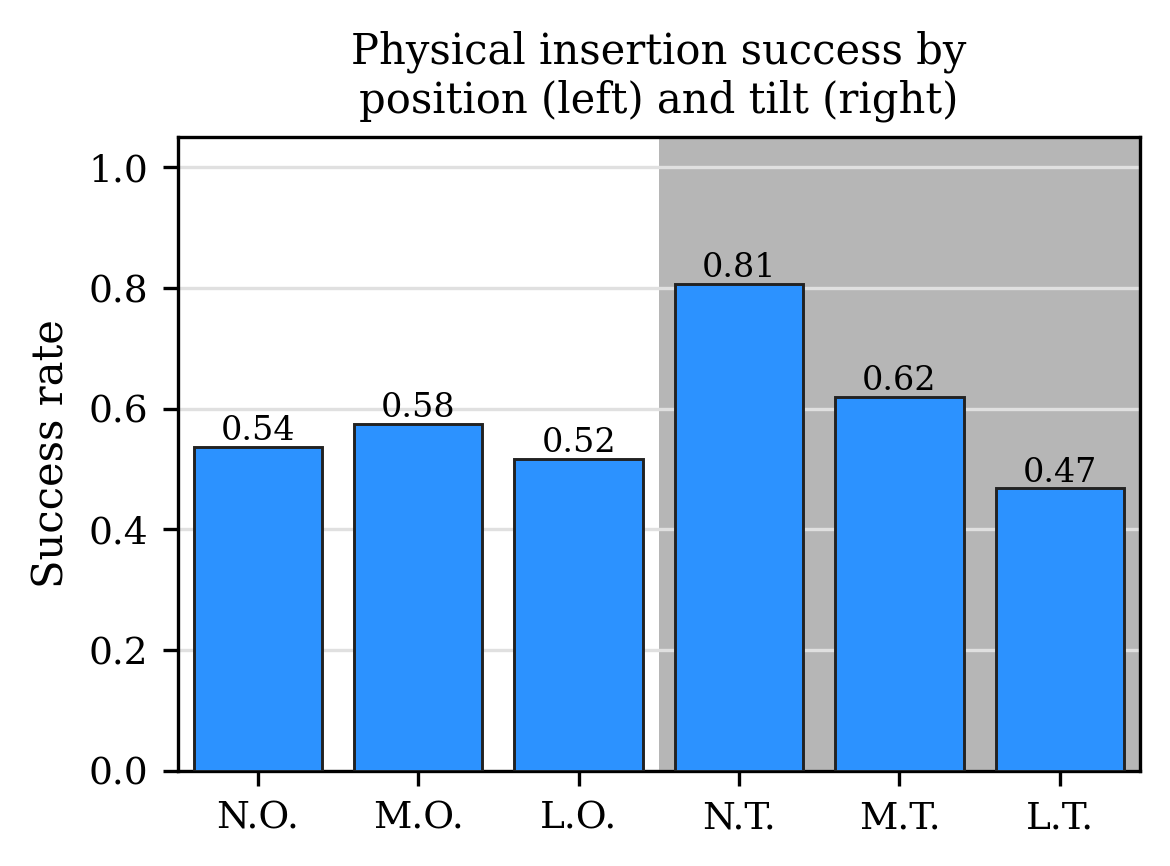
\includegraphics[width=0.95\linewidth]{chapters/7-results_and_discussion/DA1/global/physical_position_and_tilt_global.png}
        \caption{Global physical success rate for position-offset levels and tilt levels.}
        \label{fig:da1_physical_position_tilt_global}
    \end{minipage}
    \hfill
    \begin{minipage}[t]{0.45\textwidth}
        \centering
        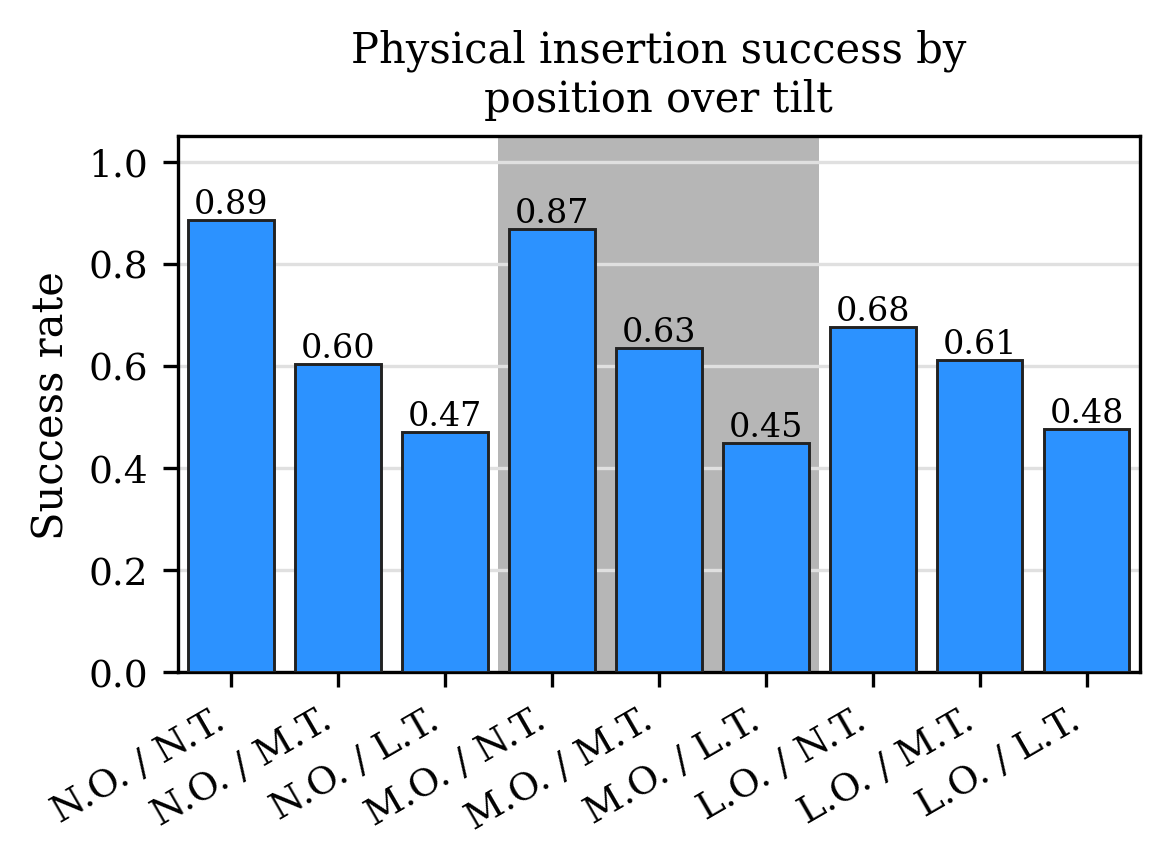
\includegraphics[width=0.95\linewidth]{chapters/7-results_and_discussion/DA1/global/physical_position_over_tilt_global.png}
        \caption{Global physical success rate for combined position--tilt groups.}
        \label{fig:da1_physical_position_over_tilt_global}
    \end{minipage}
\end{figure}

\figref{fig:da1_physical_position_tilt_global} shows the physical success rate for the individual position-offset and tilt levels. The position-offset groups alone show only low variation, with success rates between 0.52 and 0.58. In contrast, the tilt groups show a noticeable trend. Insertions without relevant tilt reach a success rate of 0.81, while moderate tilt reduces the success rate to 0.62 and large tilt further reduces it to 0.47. This indicates that angular misalignment is a more informative deviation parameter than the radial position offset alone.

The combined position--tilt groups in \figref{fig:da1_physical_position_over_tilt_global} support this interpretation. For each position-offset level, the success rate decreases as the tilt magnitude increases. No-offset insertions decrease from 0.89 for no tilt to 0.47 for large tilt, moderate-offset insertions decrease from 0.87 to 0.45, and large-offset insertions decrease from 0.68 to 0.48. The position offset therefore does not explain the success rate independently of tilt. Instead, the tilt magnitude appears to be the dominant factor in the global dataset, while the effect of position offset becomes more relevant when considered together with tilt.

The offset-direction groups in \figref{fig:da1_physical_offset_direction_global} show a smaller but still visible directional asymmetry. The positive $x$ direction has the highest success rate at 0.61, while the negative $x$ direction has the lowest success rate at 0.48. The $y$ directions lie between these values. This suggests that the insertion process may contain a setup-specific directional bias.
% However, because the differences are smaller than for the tilt groups, the direction effect is mainly treated as a secondary candidate for further investigation.

The force-related groups show a stronger effect. \figref{fig:da1_physical_force_level_and_limit_global} shows that the success rate generally decreases for high commanded force levels, especially for \texttt{F35} and \texttt{F40}. The force limit alone is less directly interpretable, because its effect depends on the force level. This becomes clear in \figref{fig:da1_physical_force_interaction_global}, where the combination of force level and force limit produces large differences in success rate. In particular, combinations where the difference between force level and force limit ($L - F$ in \figref{fig:da1_physical_force_interaction_global}) is close to zero or negative show very low success rates. Therefore, the force interaction is more informative than force level or force limit considered separately.

\begin{figure}[htbp]
    \centering
    \begin{minipage}[t]{0.45\textwidth}
        \centering
        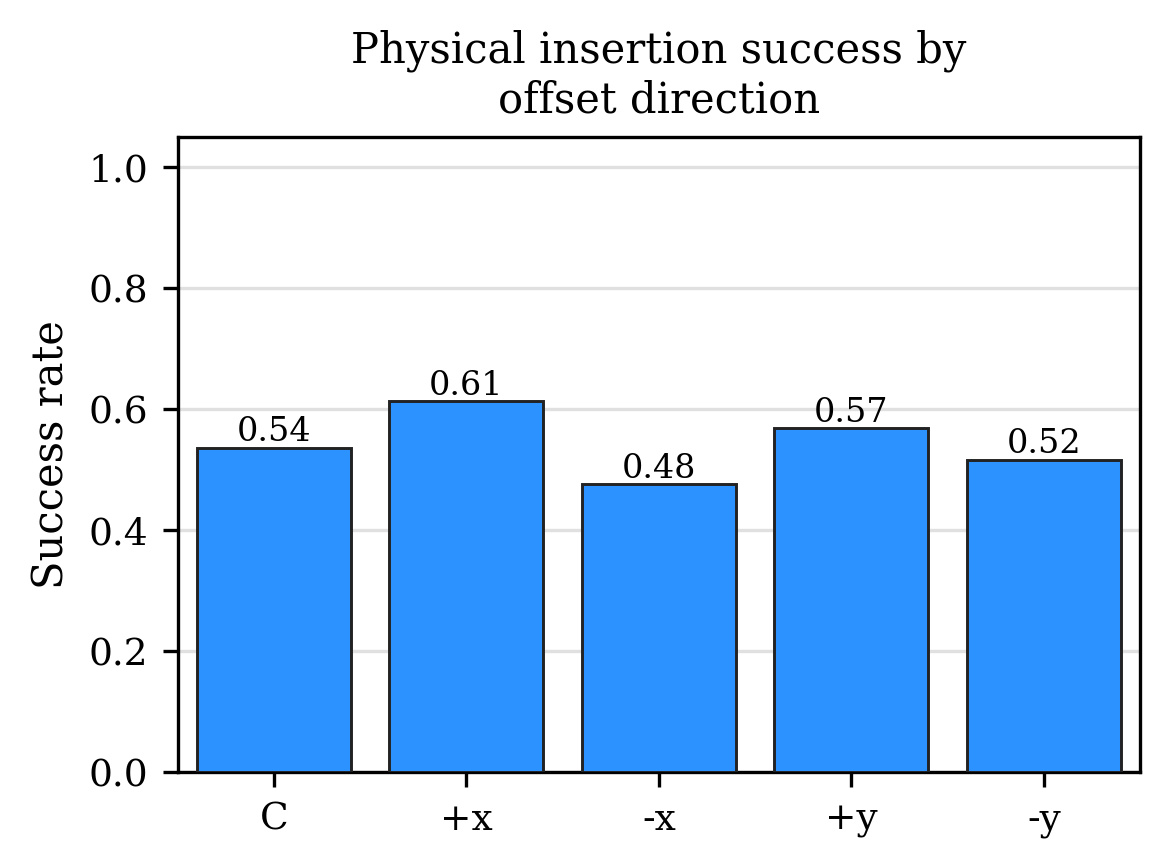
\includegraphics[width=0.9\linewidth]{chapters/7-results_and_discussion/DA1/global/physical_offset_direction_global.png}
        \caption{Global physical success rate for offset-direction groups.}
        \label{fig:da1_physical_offset_direction_global}
    \end{minipage}
    \hfill
    \begin{minipage}[t]{0.45\textwidth}
        \centering
        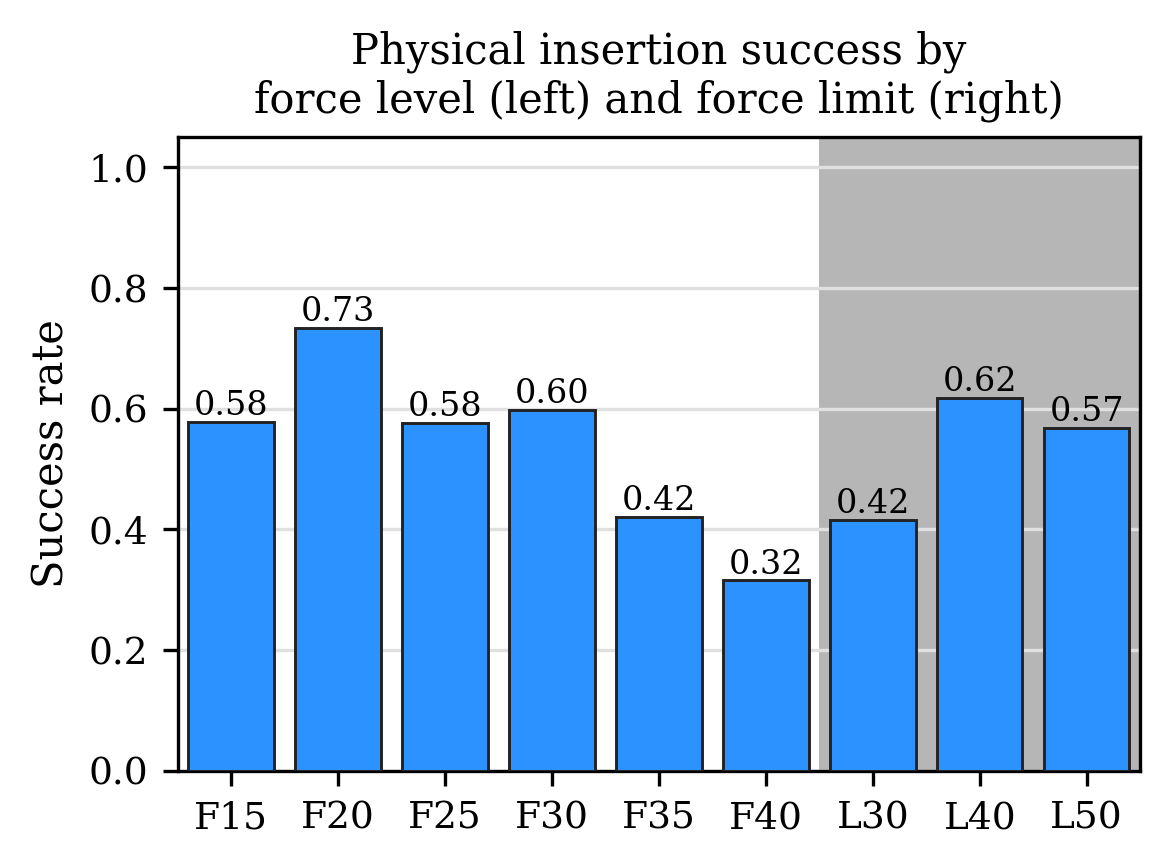
\includegraphics[width=0.9\linewidth]{chapters/7-results_and_discussion/DA1/global/physical_force_level_and_limit_global.png}
        \caption{Global physical success rate for force level and force limit.}
        \label{fig:da1_physical_force_level_and_limit_global}
    \end{minipage}
\end{figure}

\begin{figure}[htbp]
    \centering
    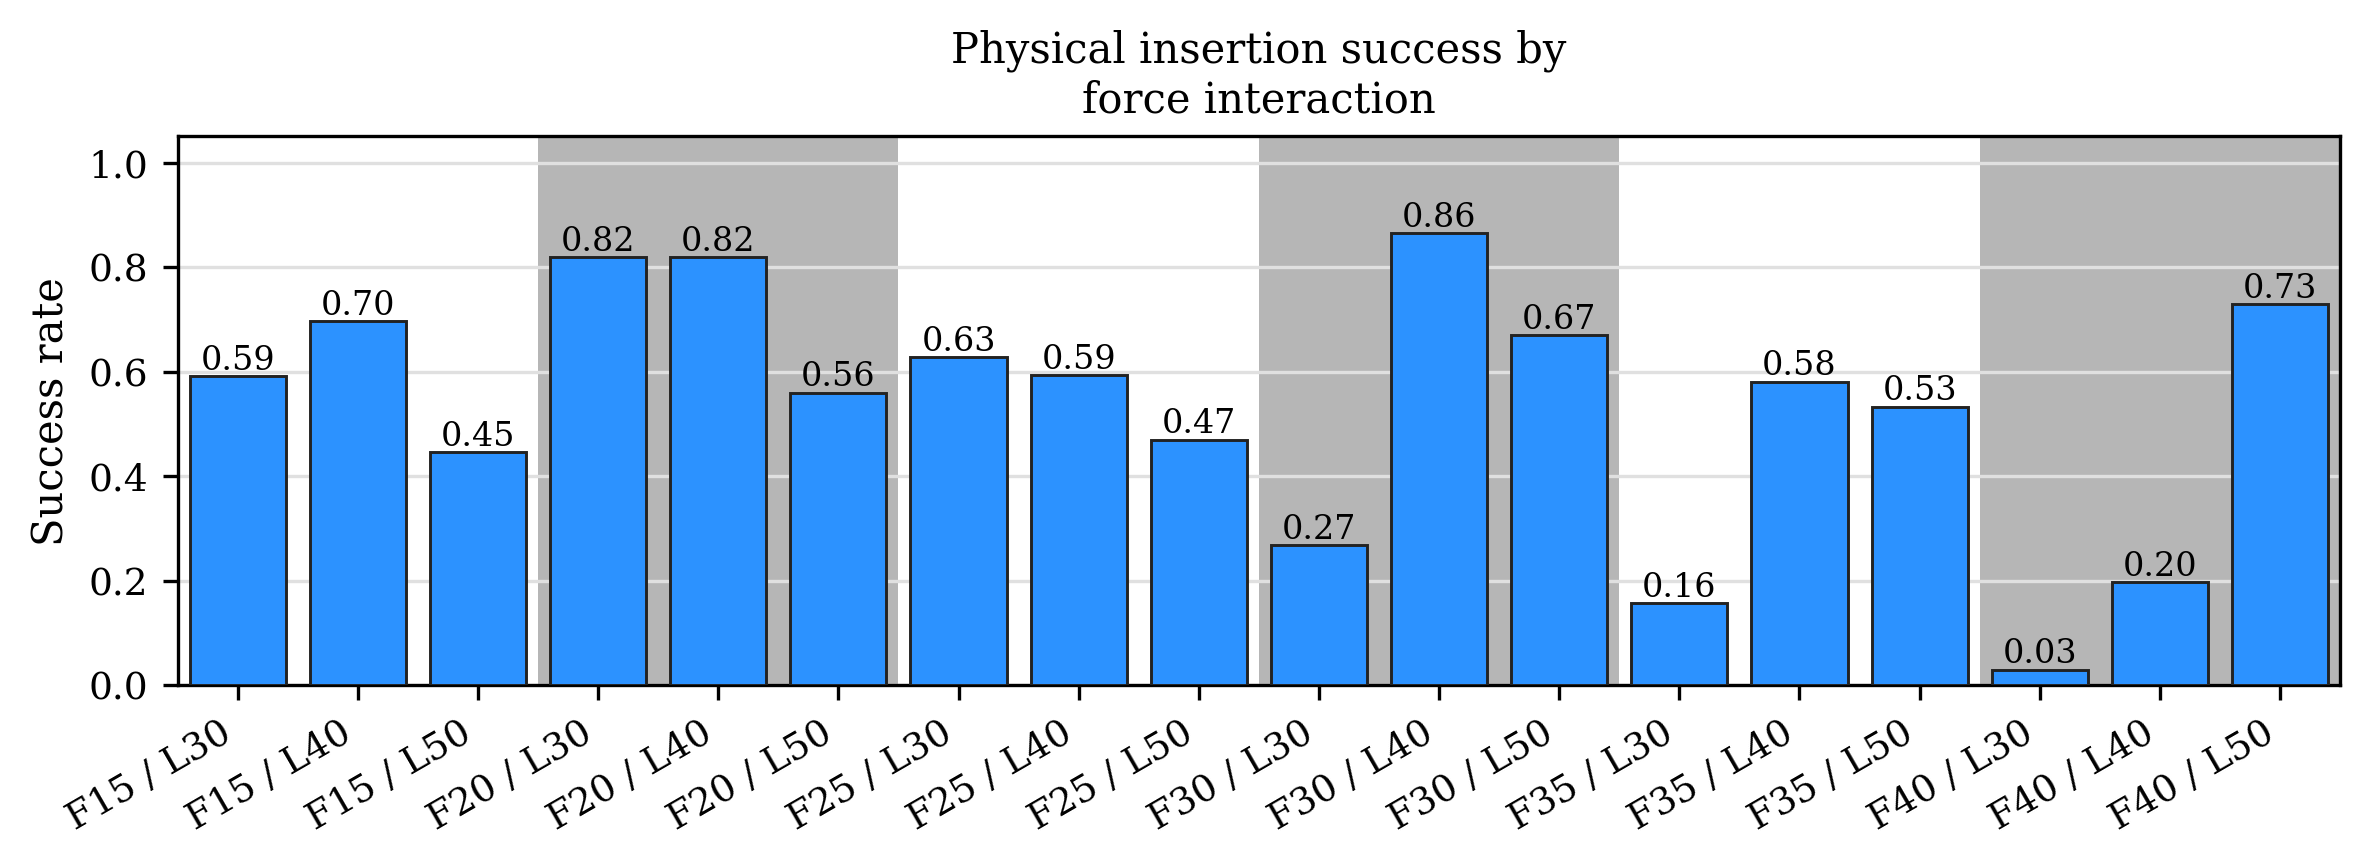
\includegraphics[width=0.9\linewidth]{chapters/7-results_and_discussion/DA1/global/physical_force_interaction_global.png}
    \caption{Global physical success rate for force-interaction groups.}
    \label{fig:da1_physical_force_interaction_global}
\end{figure}

\newpage

To further investigate the force interaction, two subsets are shown in \figref{fig:da1_physical_force_no_tilt_no_offset} and \figref{fig:da1_physical_position_tilt_f40_l30}. The first subset in \figref{fig:da1_physical_force_no_tilt_no_offset} considers only insertions without relevant position offset and without relevant tilt. Due to limitations of the deviation planner explained in Section \ref{sec:dataset_collection}, the force limits \texttt{L30} and \texttt{L50} were not recorded with no tilt and no offset, which means that all force levels (\texttt{F15 - F40}) had the force limit \texttt{L40} during insertions. In this specific subset,the force interaction levels \texttt{F15/L40}, \texttt{F20/L40}, \texttt{F25/L40}, and \texttt{F30/L40} reach a physical success rate of 1.0. This indicates that, in the absence of relevant translational and angular misalignment, several force settings are sufficient for reliable insertion. However, the success rate decreases for higher force levels, especially for \texttt{F40}.

The opposite case is shown in \figref{fig:da1_physical_position_tilt_f40_l30}, where the force interaction is fixed to \texttt{F40/L30}, resulting in a force difference of $30 - 40 = -10$N. Across the available position--tilt groups, the physical success rate remains close to zero. This confirms that the low success rate of \texttt{F40/L30} is not caused by a single position--tilt group alone, but is a generally unfavorable force interaction in the recorded dataset. This result supports the interpretation that the force limit is likely exceeded before the insertion can be completed, when the force level is too close to or above the allowed force limit.

\begin{figure}[htbp]
    \centering
    \begin{minipage}[t]{0.49\textwidth}
        \centering
        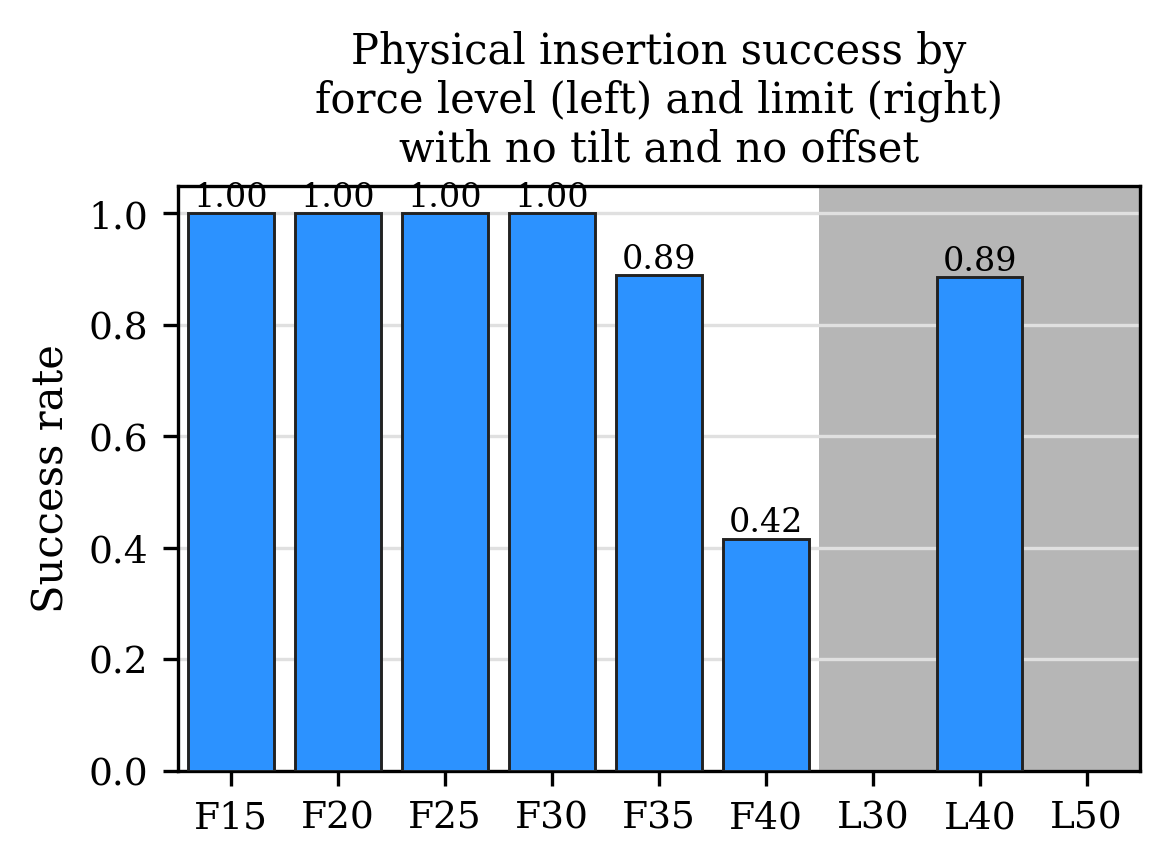
\includegraphics[width=0.99\linewidth]{chapters/7-results_and_discussion/DA1/global/physical_F_L_NT_NO_global.png}
        \caption{Physical success rate for force level and force limit under no tilt and no offset. Missing bars indicate that no samples were available for the corresponding force-limit level in this subset.}
        \label{fig:da1_physical_force_no_tilt_no_offset}
    \end{minipage}
    \hfill
    \begin{minipage}[t]{0.49\textwidth}
        \centering
        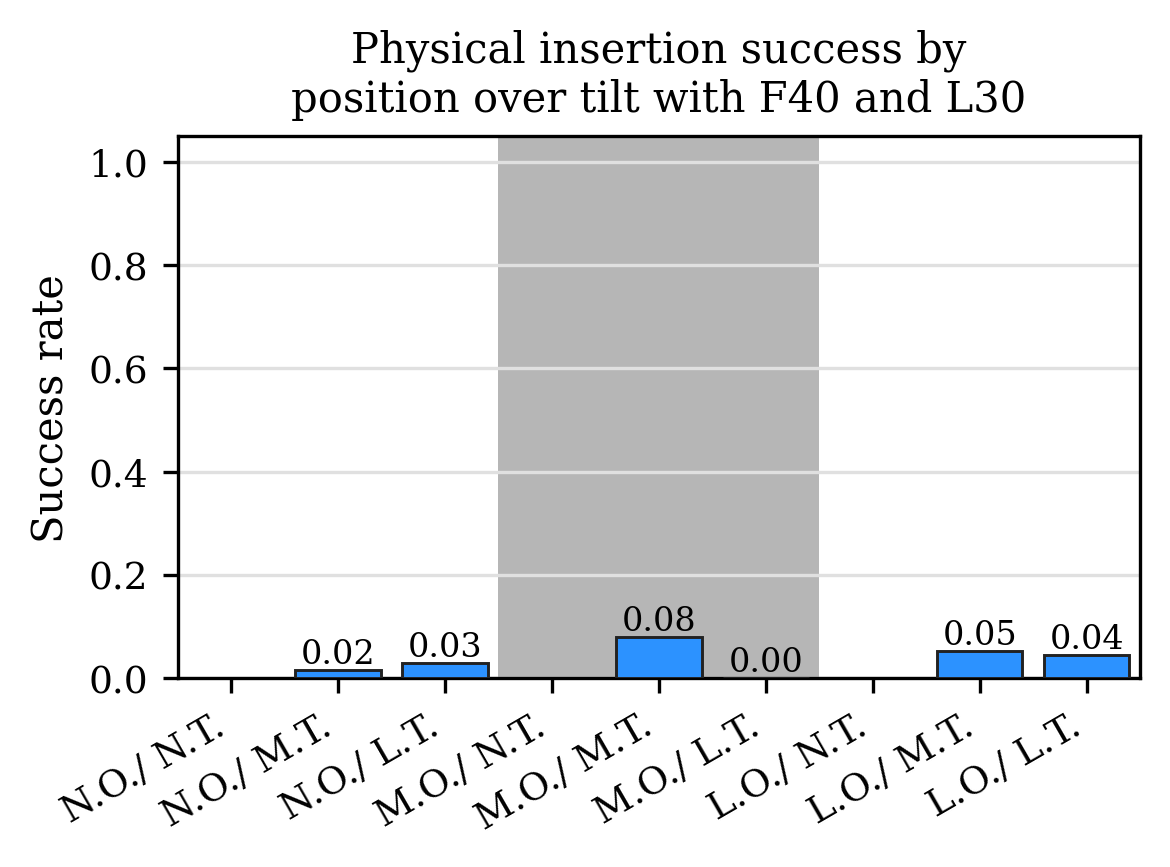
\includegraphics[width=0.99\linewidth]{chapters/7-results_and_discussion/DA1/global/physical_position_over_tilt_F40_L30_global.png}
        \caption{Physical success rate of position--tilt groups for the force interaction \texttt{F40/L30}. Missing bars indicate unavailable deviation combinations in this subset.}
        \label{fig:da1_physical_position_tilt_f40_l30}
    \end{minipage}
\end{figure}

The record offset in \figref{fig:da1_physical_record_offset_global} shows a gradual increase in success rate from the early to the late recording windows. This group is reported for completeness, but it is not interpreted as a physical cause of insertion success or failure.

Finally, \figref{fig:da1_physical_grasp_approach_height_global} shows that grasp height and approach height have comparatively low global effects. The grasp height differs slightly between 0 mm and 7 mm, while the three approach-height levels show almost identical success rates.

The sample counts and class balances for all global deviation groups are listed in \tabref{tab:da1_class_split_global}. The table shows that the deviation groups are not equally sized. This is especially visible for the tilt groups, where the large-tilt group contains substantially more samples than the no-tilt group. This imbalance is due to the goal to have balanced class splits for all levels in a deviation group. \figref{fig:da1_sankey_tilt} visualizes this split exemplarily for the tilt groups and shows how the complete dataset is divided into tilt levels and physical insertion outcomes. This principle holds for every deviation group.

Overall, the global screening identifies tilt magnitude and force interaction as the most relevant deviation groups for further investigation. Offset direction is also considered because it indicates a possible directional asymmetry. In contrast, grasp height and approach height show only weak global effects and are therefore not investigated in detail in the following domain-specific analysis.


\begin{figure}[htbp]
    \centering
    \begin{minipage}[t]{0.45\textwidth}
        \centering
        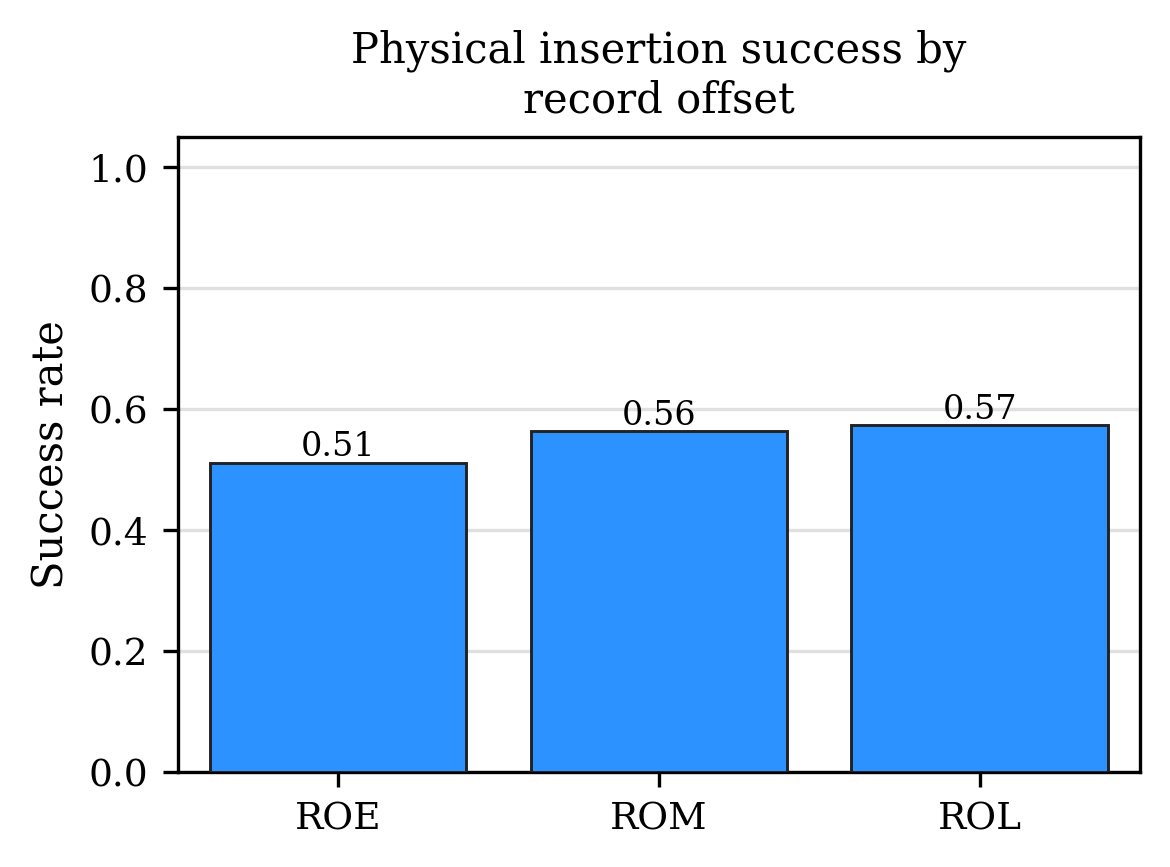
\includegraphics[width=0.9\linewidth]{chapters/7-results_and_discussion/DA1/global/physical_record_offset_global.png}
        \caption{Global physical success rate for record-offset groups.}
        \label{fig:da1_physical_record_offset_global}
    \end{minipage}    
    \hfill
    \begin{minipage}[t]{0.45\textwidth}
        \centering
        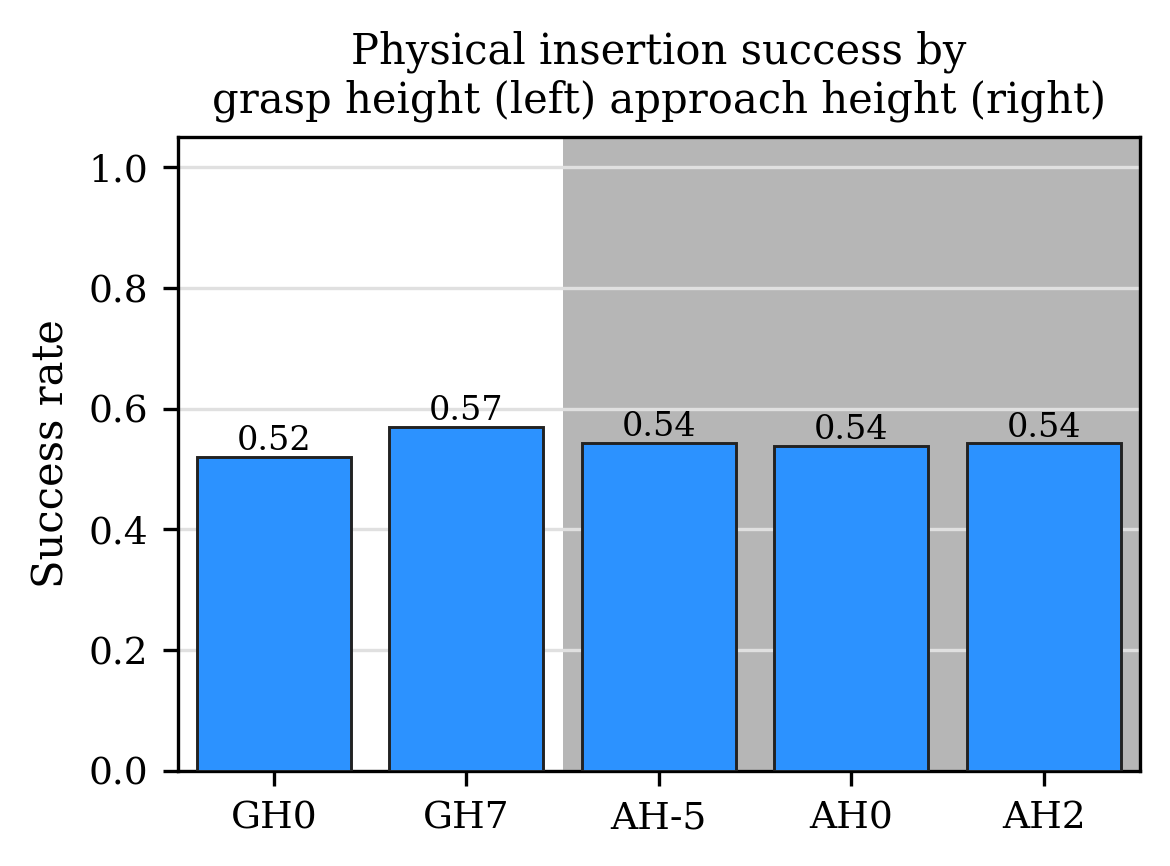
\includegraphics[width=0.9\linewidth]{chapters/7-results_and_discussion/DA1/global/physical_grasp_approach_height_global.png}
        \caption{Global physical success rate for grasp height and approach height.}
        \label{fig:da1_physical_grasp_approach_height_global}
    \end{minipage}    
\end{figure}

\begin{figure}[htbp]
    \centering
    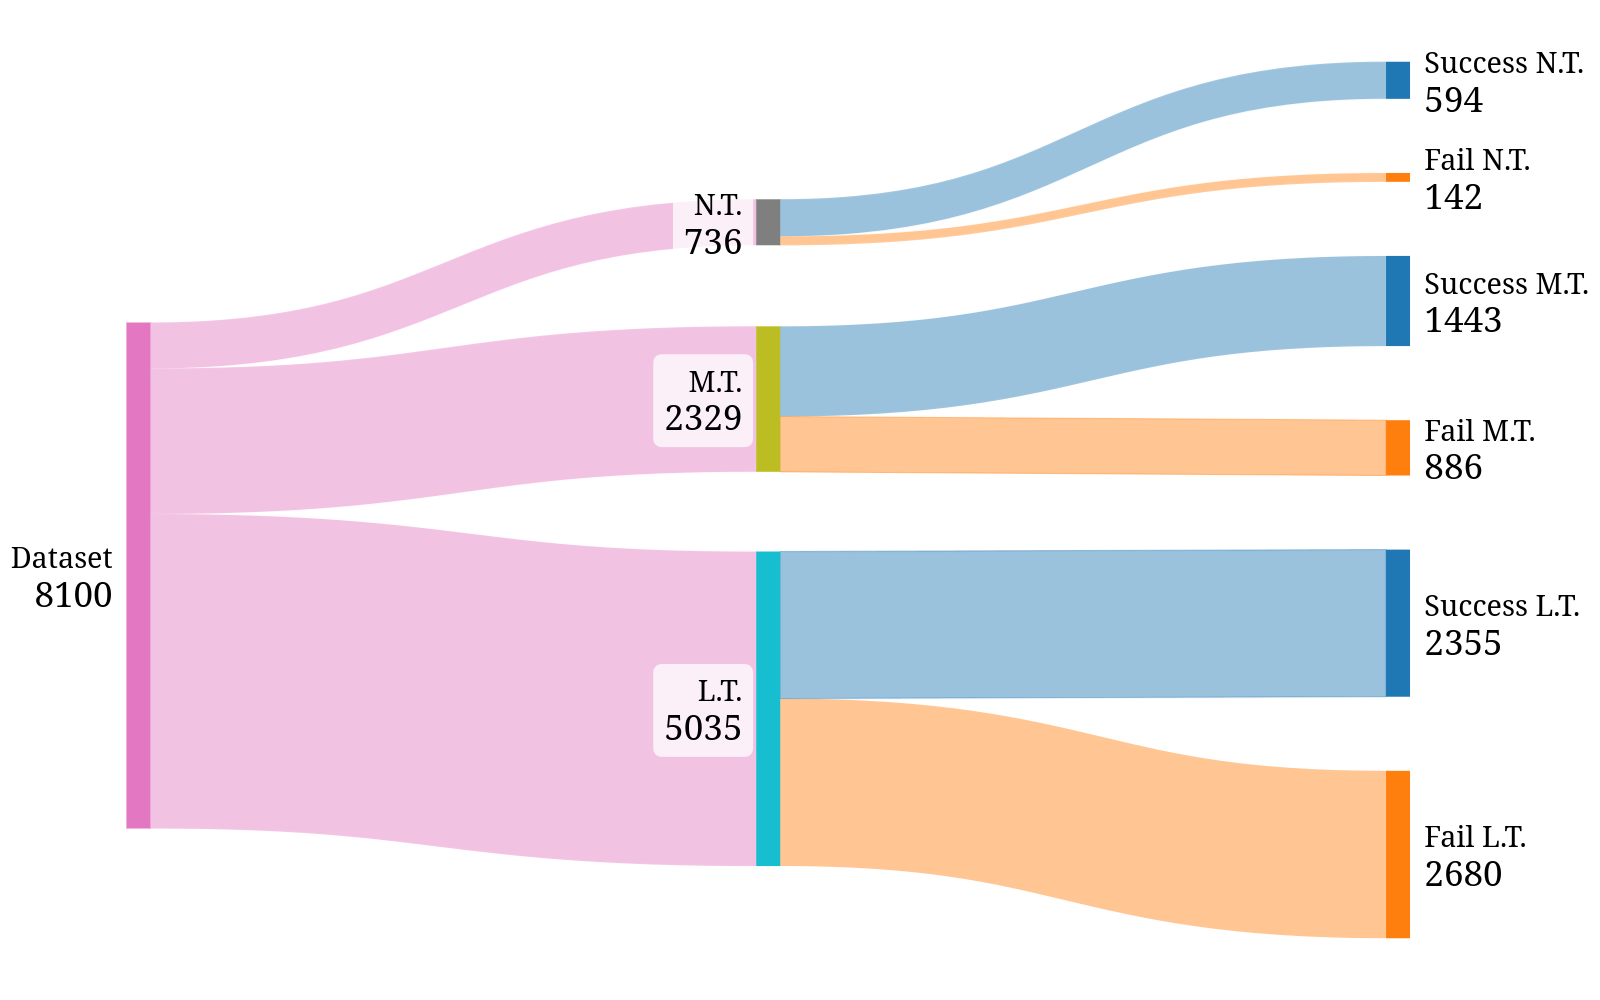
\includegraphics[width=0.8\linewidth]{chapters/7-results_and_discussion/DA1/global/sankey_tilt.png}
    \caption{Example Sankey diagram showing the split of the complete dataset into tilt groups and physical insertion outcomes.}
    \label{fig:da1_sankey_tilt}
\end{figure}

\begin{table}[htbp]
    \centering
    \caption{Sample counts and class balance for the global deviation groups used in Deviation Analysis I.}
    \label{tab:da1_class_split_global}
    \begin{tabular}{l lll lll}
        \toprule
        \textbf{Deviation group} & \textbf{LV} & \textbf{\#} & \textbf{(pos, neg)} & \textbf{LV} & \textbf{\#} & \textbf{(pos, neg)}\\
        \midrule

        \texttt{position} & N.O. & 3150 & (1688, 1462) & M.O. & 2484 & (1429, 1055) \\
        & L.O. & 2466 & (1275, 1191) \\
        \midrule
        \texttt{tilt} & N.T. & 736 & (594, 142) & M.T. & 2329 & (1443, 886) \\
        & L.T. & 5035 & (2355, 2680) \\
        \midrule
        \texttt{offset\_direction} & C & 3150 & (1688, 1462) & pos x & 1328 & (813, 515) \\
        & neg x & 1146 & (545, 601) & pos y & 1319 & (749, 570) \\
        & neg y & 1157 & (597, 560) \\
        \midrule
        \texttt{force\_level} & F15 & 1180 & (682, 498) & F20 & 1220 & (895, 325) \\
        & F25 & 2100 & (1211, 889)  & F30 & 1211& (724, 487) \\
        & F35 & 1200 & (505, 695) & F40 & 1189 & (375, 814) \\
        \midrule
        \texttt{force\_limit} & L30 & 2448 & (1019, 1429) & L40 & 3276 & (2023, 1253) \\
        & L50 & 2376 & (1350, 1026) \\
        \midrule
        \texttt{record\_offset} & ROE & 3780 & (1930, 1850) & ROM & 1440 & (811, 629) \\
        & ROL & 2880 & (1651, 1229) \\
        \midrule
        \texttt{grasp\_height} & 0 mm & 4500 & (2342, 2158) & 7 mm & 3600 & (2050, 1550) \\
        \midrule
        \texttt{approach\_height} & -5 mm & 3649 & (1982, 1667) & 0 mm & 900 & (484, 416) \\
        & 2 mm & 3551 & (1926, 1625) \\
        \midrule
        \texttt{position\_tilt} & N.O./N.T. & 218 & (193, 25) & N.O./M.T. & 866 & (523, 343) \\
        & N.O./L.T. & 2066 & (972, 1094) & M.O./N.T. & 265 & (230, 35) \\
        & M.O./M.T. & 1087 & (690, 397) & M.O./L.T. & 1132 & (509, 623) \\
        & L.O./N.T. & 253 & (171, 82) & L.O./M.T. & 376 & (230, 146) \\
        & L.O./L.T. & 1837 & (874, 963) \\
        \midrule
        \texttt{force\_interaction} & F15/L30 & 401 & (237, 164) & F15/L40 & 389 & (271, 118) \\
        & F15/L50 & 390 & (174, 216) & F20/L30 & 415 & (340, 75) \\
        & F20/L40 & 403 & (330, 73) & F20/L50 & 402 & (225, 177) \\
        & F25/L30 & 408 & (256, 152) & F25/L40 & 1296 & (769, 527) \\
        & F25/L50 & 396 & (186, 210) & F30/L30 & 411 & (110, 301) \\
        & F30/L40 & 400 & (346, 54) & F30/L50 & 400 & (268, 132) \\
        & F35/L30 & 408 & (64,344) & F35/L40 & 396 & (230, 166) \\
        & F35/L50 & 396 & (211, 185) & F40/L30 & 405 & (12,393) \\
        & F40/L40 & 392 & (77, 315) & F40/L50 & 392 & (286, 106) \\
        \midrule
        \figref{fig:da1_physical_force_no_tilt_no_offset} Attributes &
        F15 & 35 & (35, 0) & F20 & 37 & (37, 0) \\
        & F25 & 38 & (38, 0) & F30 & 36 & (36, 0) \\
        & F35 & 36 & (32, 4) & F40 & 36 & (15, 21) \\
        & L30 & 0 & (0, 0) & L40 & 218 & (193, 25) \\
        & L50 & 0 & (0, 0) \\
        \midrule
        \figref{fig:da1_physical_position_tilt_f40_l30} Attributes &
        N.O./N.T. & 0 & (0, 0) & N.O./M.T. & 65 & (1, 64) \\
        & N.O./L.T. & 173 & (5, 168) & M.O./N.T. & 0 & (0, 0) \\
        & M.O./M.T. & 25 & (2, 23) & M.O./L.T. & 56 & (0, 56) \\
        & L.O./N.T. & 0 & (0, 0) & L.O./M.T. & 19 & (1, 18) \\
        & L.O./L.T. & 67 & (3, 64) \\
        \bottomrule
    \end{tabular}
\end{table}

\newpage
% MARK: DA1 Domain
\subsection{Domain specific Investigation of Deviation Groups}
\label{subsec:da1_domain_investigation}

The global investigation identified tilt magnitude, offset direction, and force interaction as the most informative deviation groups for the physical success-rate analysis. These groups are therefore investigated further on selected dataset domains. The purpose of this second part is to determine whether the global effects are consistent across hole configurations, or whether they are caused by specific rod--tolerance combinations, gripper configurations, or batch-dependent recording conditions.

The analysis is focused on the hole domains, defined by the combination of \texttt{rod\_type} and \texttt{tolerance}. Additional focused investigations are then performed for domains that show particularly strong or unexpected behavior.

\subsubsection{Hole-Domain Screening}
\label{subsubsec:da1_hole_domain_screening}

\figref{fig:da1_domain_position_tilt_holes} shows the physical success rate of the individual position-offset and tilt groups across the nine hole domains. The domain-specific view confirms the global observation that tilt is more impactful than position offset alone. Across most hole domains, the no-tilt group has the highest success rate, while large tilt causes the success rate to drop. 8 out of 9 hole domains follow the consisten trend:

\begin{equation}
    \text{SR}(\texttt{N.T.}) > \text{SR}(\texttt{M.T.}) > \text{SR}(\texttt{L.T.})
    \qquad
    \text{SR}() := \texttt{Success Rate()}.
    \label{eq:tilt_trend}
\end{equation}
\texttt{small\_rod\_t0.2} is the only case where $\text{SR}(\texttt{M.T.}) < \text{SR}(\texttt{L.T.})$.

\begin{figure}[htbp]
    \centering
    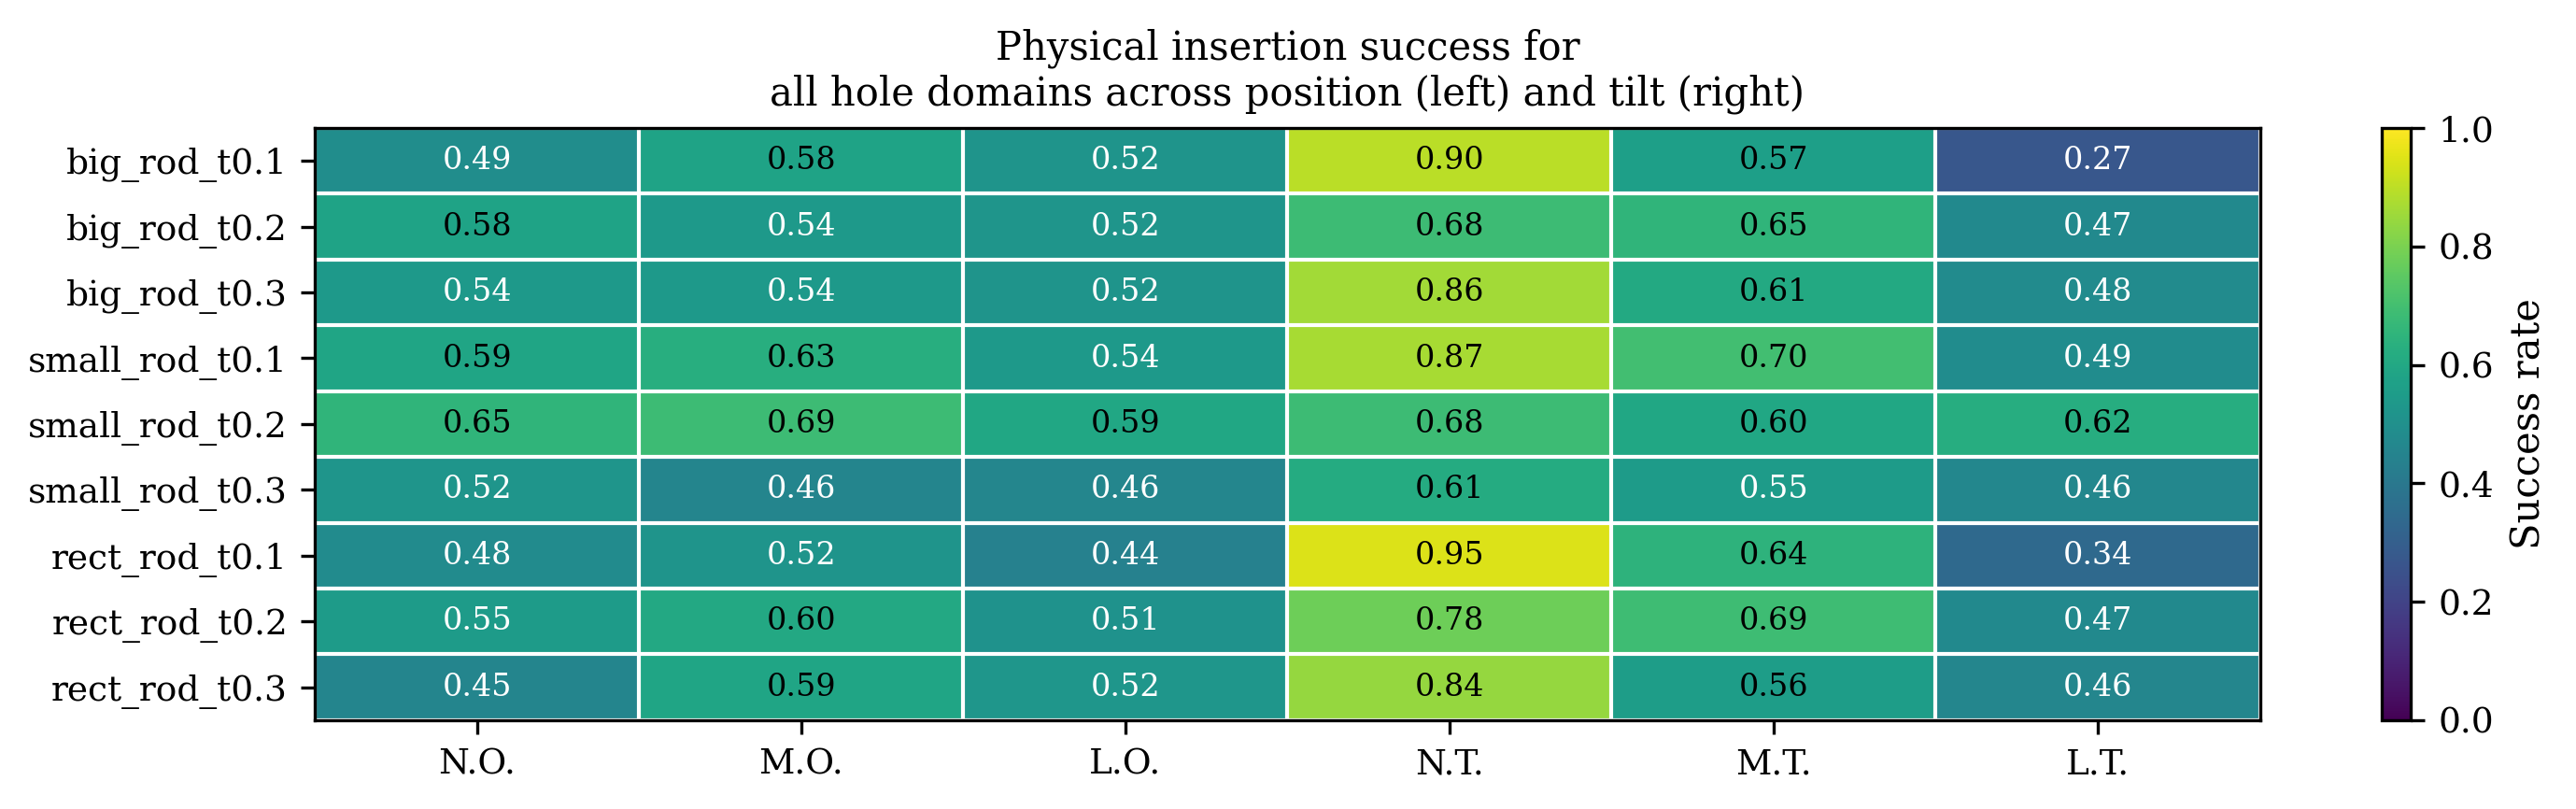
\includegraphics[width=0.95\linewidth]{chapters/7-results_and_discussion/DA1/domain/physical_hole_domains_position_and_tilt.png}
    \caption{Physical success rate of position-offset and tilt groups across all hole domains.}
    \label{fig:da1_domain_position_tilt_holes}
\end{figure}

In contrast, the position-offset groups do not show the same consistent decline of success rate. No offset is not always clearly superior to moderate or large offset, which indicates that positional offset magnitude alone is not sufficient to explain the physical outcome.

\begin{figure}[htbp]
    \centering
    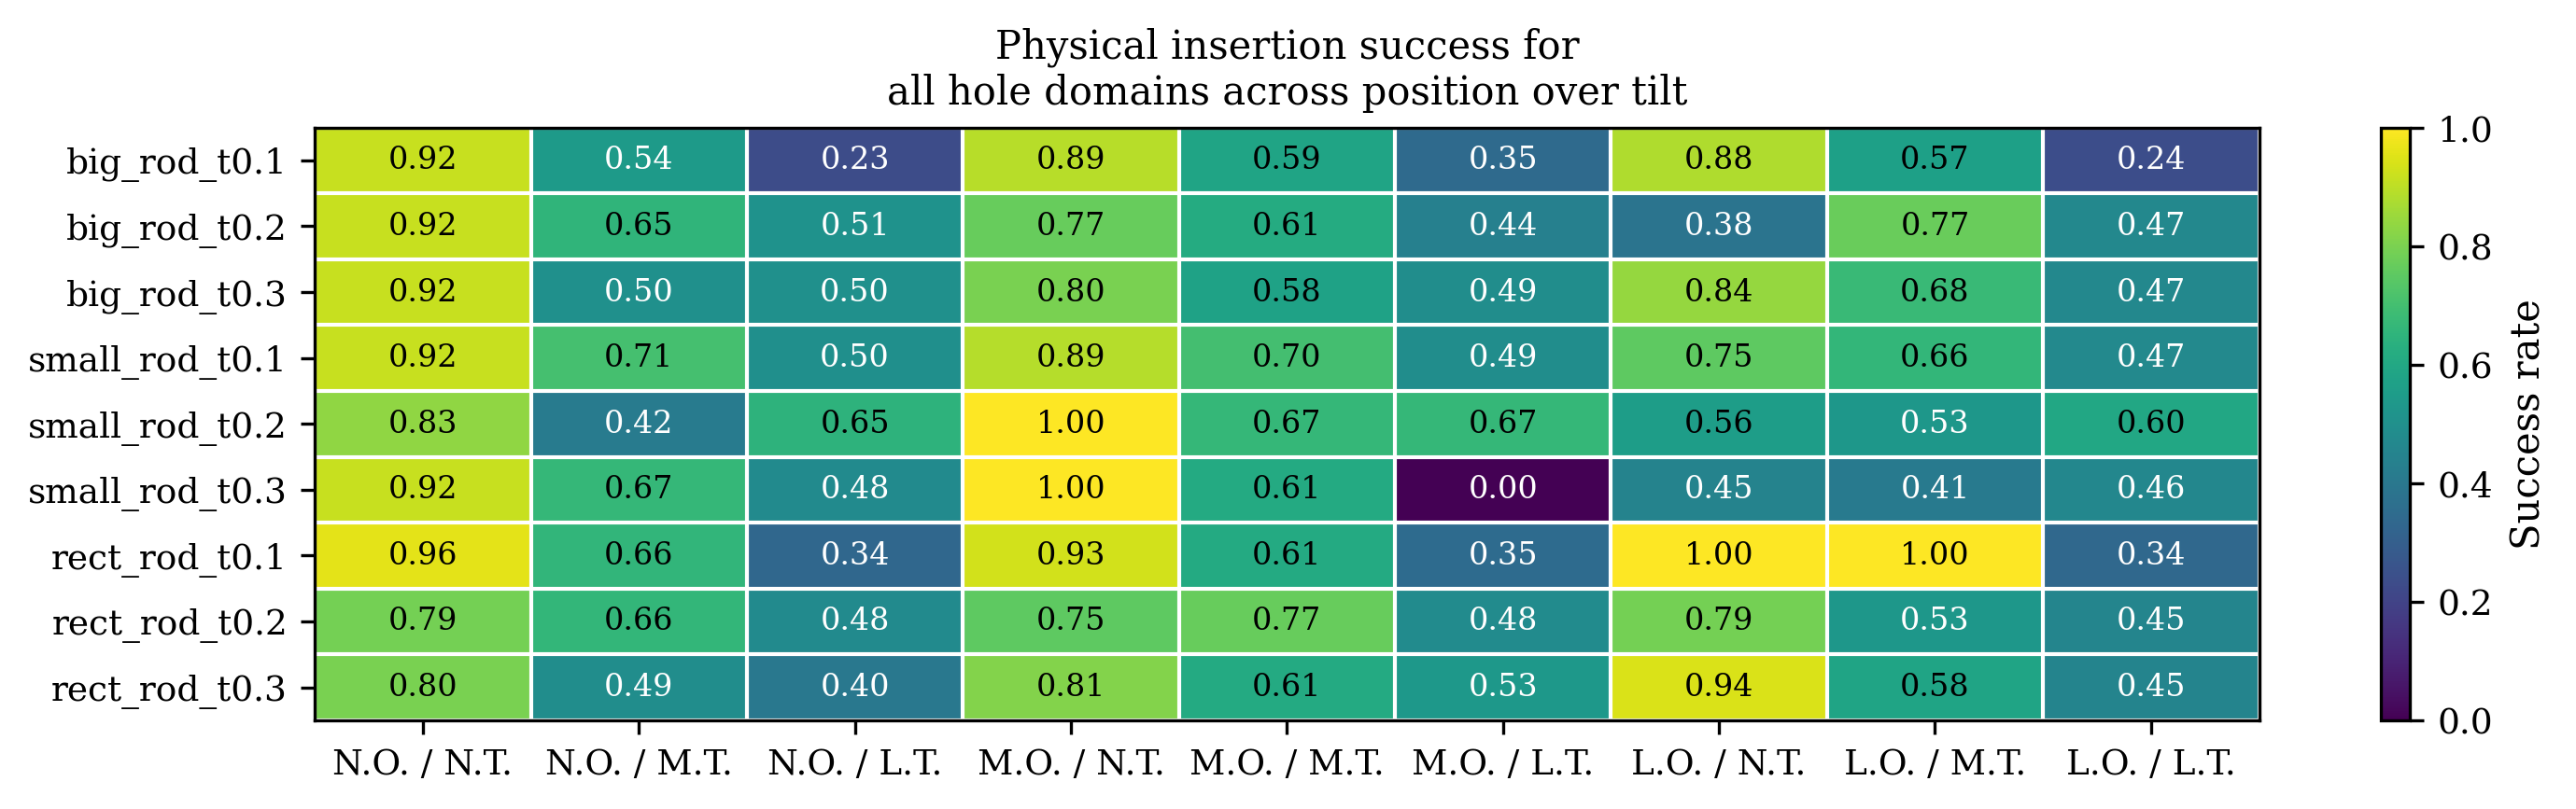
\includegraphics[width=0.95\linewidth]{chapters/7-results_and_discussion/DA1/domain/physical_hole_domains_position_over_tilt.png}
    \caption{Physical success rate of combined position--tilt groups across all hole domains.}
    \label{fig:da1_domain_position_over_tilt_holes}
\end{figure}

The combined position--tilt groups in \figref{fig:da1_domain_position_over_tilt_holes} provide a more detailed view of this effect. The highest success rates occur mostly in groups where no-tilt is involved, especially for the no-offset with no-tilt case. However, the effect is not identical in all hole domains. Some combinations are missing due to the deterministic structure of the deviation planner, and some domains show local patterns that differ from the global trend. In particular, \texttt{small\_rod\_t0.3} shows no samples for \texttt{M.O./N.T.} and a very low success rate for \texttt{M.O./L.T.}. 

\begin{figure}[htbp]
    \centering
    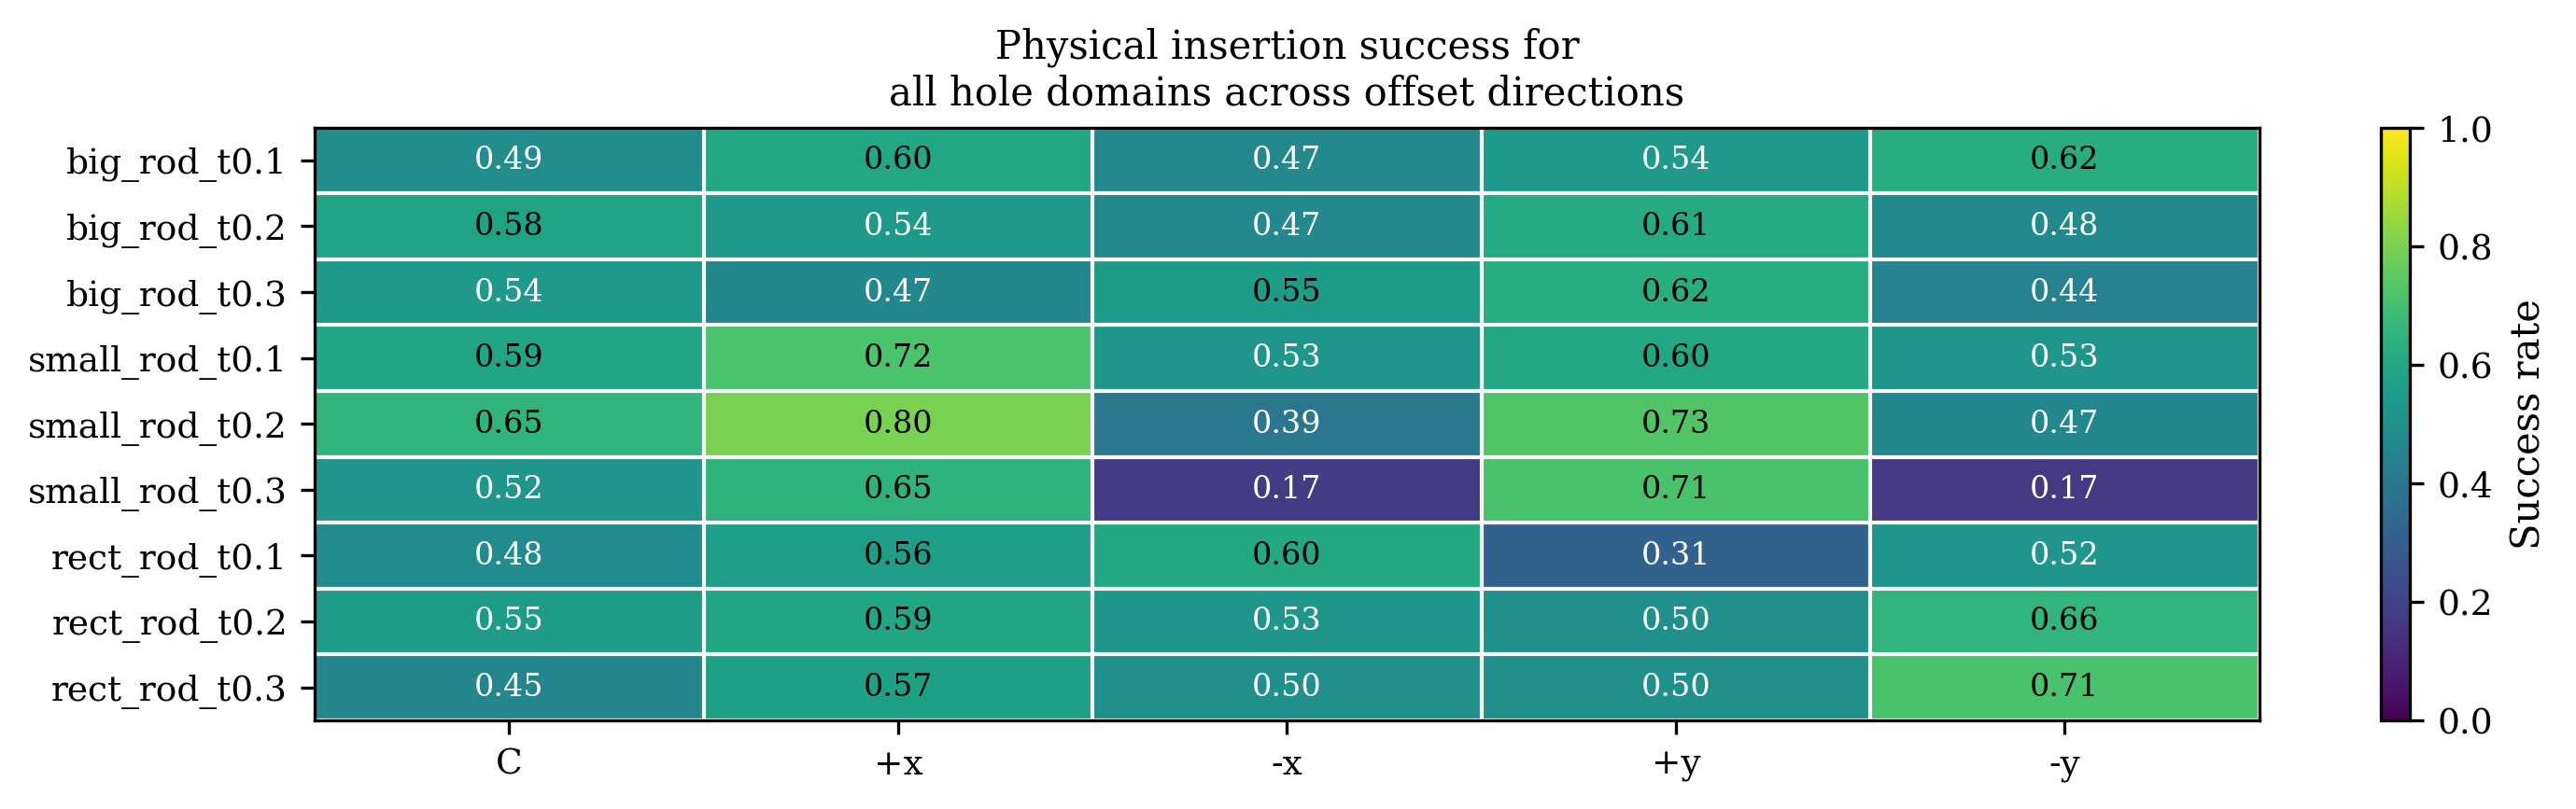
\includegraphics[width=0.95\linewidth]{chapters/7-results_and_discussion/DA1/domain/physical_hole_domains_offset_direction.png}
    \caption{Physical success rate of offset-direction groups across all hole domains.}
    \label{fig:da1_domain_offset_direction_holes}
\end{figure}

\figref{fig:da1_domain_offset_direction_holes} shows the hole domain specific view on the success rate of the five offset-directions. The domain \texttt{small\_rod\_t0.3} shows unexpected behavior, where offsets in the negative $x$ and negative $y$ directions are associated with much lower success rates than offsets in the positive directions. This could reveal a directional bias or asymmetry in the robotic setup. If the targeted insertion pose without deviations applied, is slightly shifted relative to the ground truth hole center, repeated deviations in one direction can show different behavior than deviations in the opposite direction.

Because of these two anomalies regarding \texttt{small\_rod\_t0.3}, this domain is further investigated.

\begin{figure}[htbp]
    \centering
    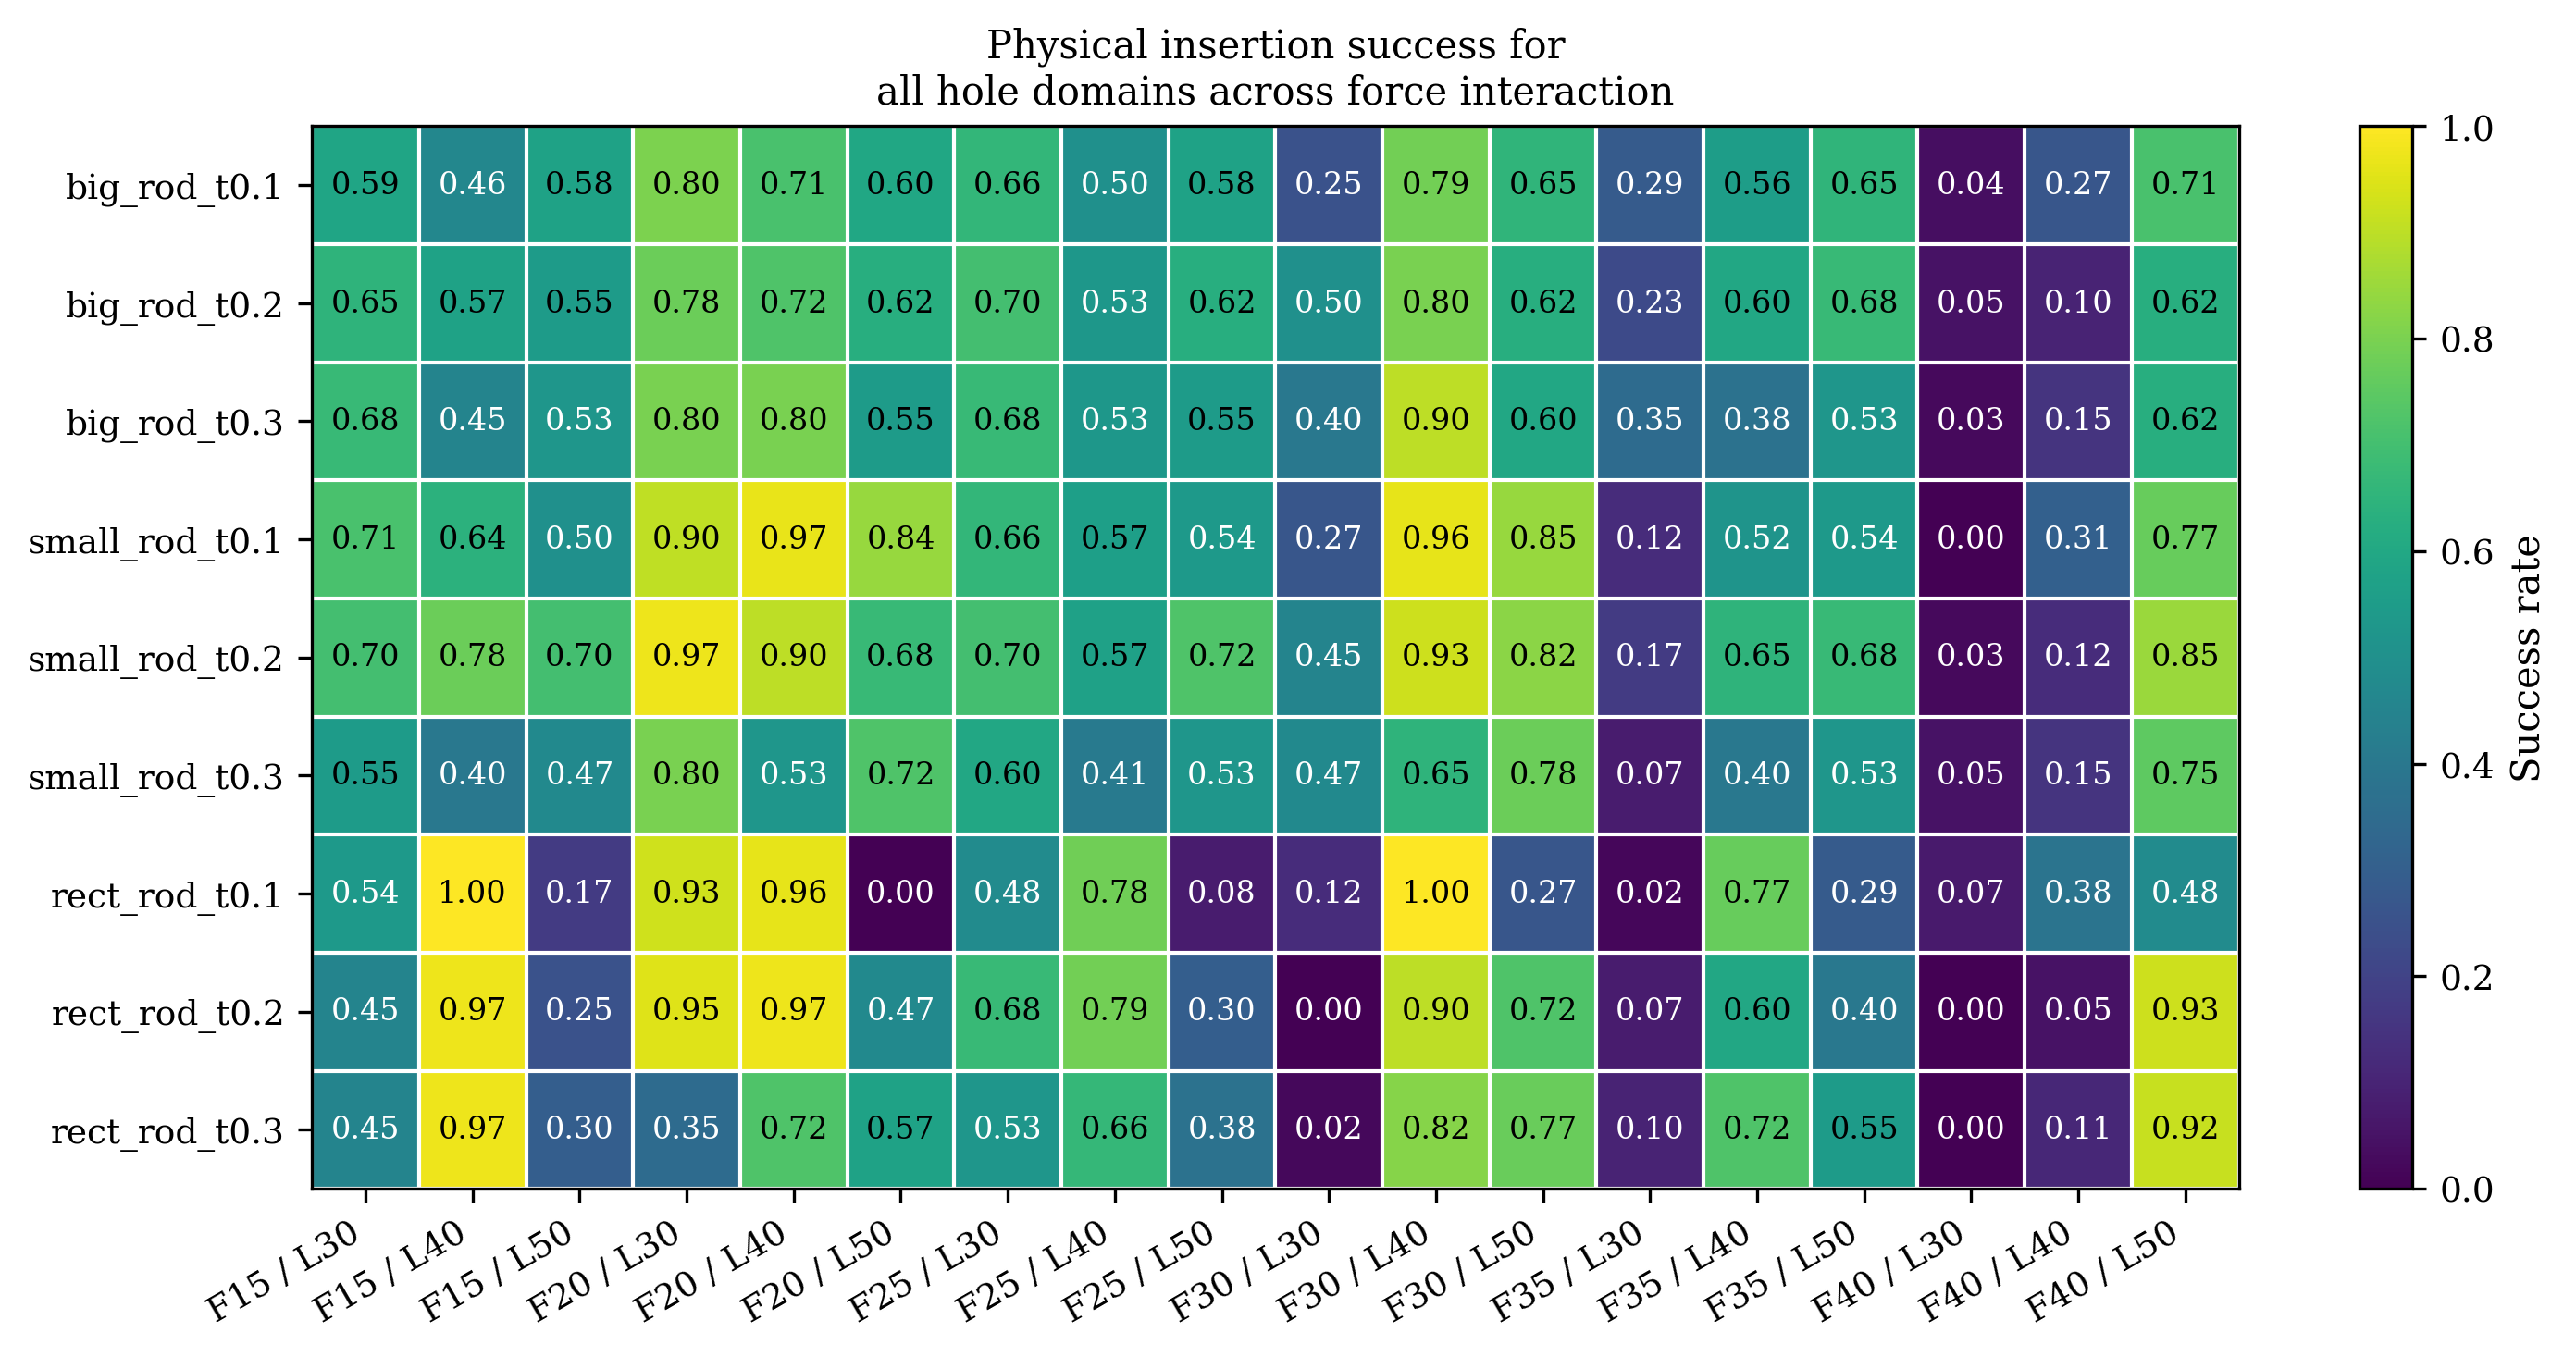
\includegraphics[width=0.95\linewidth]{chapters/7-results_and_discussion/DA1/domain/physical_hole_domains_force_interaction.png}
    \caption{Physical success rate of force-interaction groups across hole domains.}
    \label{fig:da1_domain_force_interaction_holes}
\end{figure}

The force-interaction heatmap in \figref{fig:da1_domain_force_interaction_holes} shows particularly stronger variation across hole domains. The combination \texttt{F40/L30} remains one of the least successful settings across several hole domains, which is consistent with the global result in \figref{fig:da1_physical_force_interaction_global}. This setting combines the highest commanded force level with the lowest force limit, so the force limit is likely to be reached before the insertion can be completed. At the same time, the heatmap shows that the force interaction global pattern does not apply to all hole domains. The \texttt{rect\_rod\_t0.1} domain in particular shows extreme differences, with some force interactions leading to almost complete success (\texttt{F20/L40}) with direclty adjacent force interactions leading to almost complete failure (\texttt{F20/L50}). This motivated the second focused investigation of \texttt{rect\_rod\_t0.1}.



For the focused investigations, the heatmap tiles are extended with additional failure-mode information. This comes from the metadata entry \texttt{failure\_reason} in \tabref{tab:recorded_metadata} and its description in Section \ref{sec:dataset_labeling}. Besides the success rate, each tile reports the number of samples $n$ and the distribution of failure reasons. The abbreviation \texttt{T} denotes the count of timeouts, \texttt{F} denotes the count of force-limit reached failures, and \texttt{S} counts the amounf of stall/jam failures. These failure modes allow the success rate to be interpreted more precisely, because a failed insertion can result from different physical mechanisms.

\subsubsection{Directional Bias in \texttt{small\_rod\_t0.3}}
\label{subsubsec:da1_small_rod_t03_directional_bias}

\begin{figure}[htbp]
    \centering
    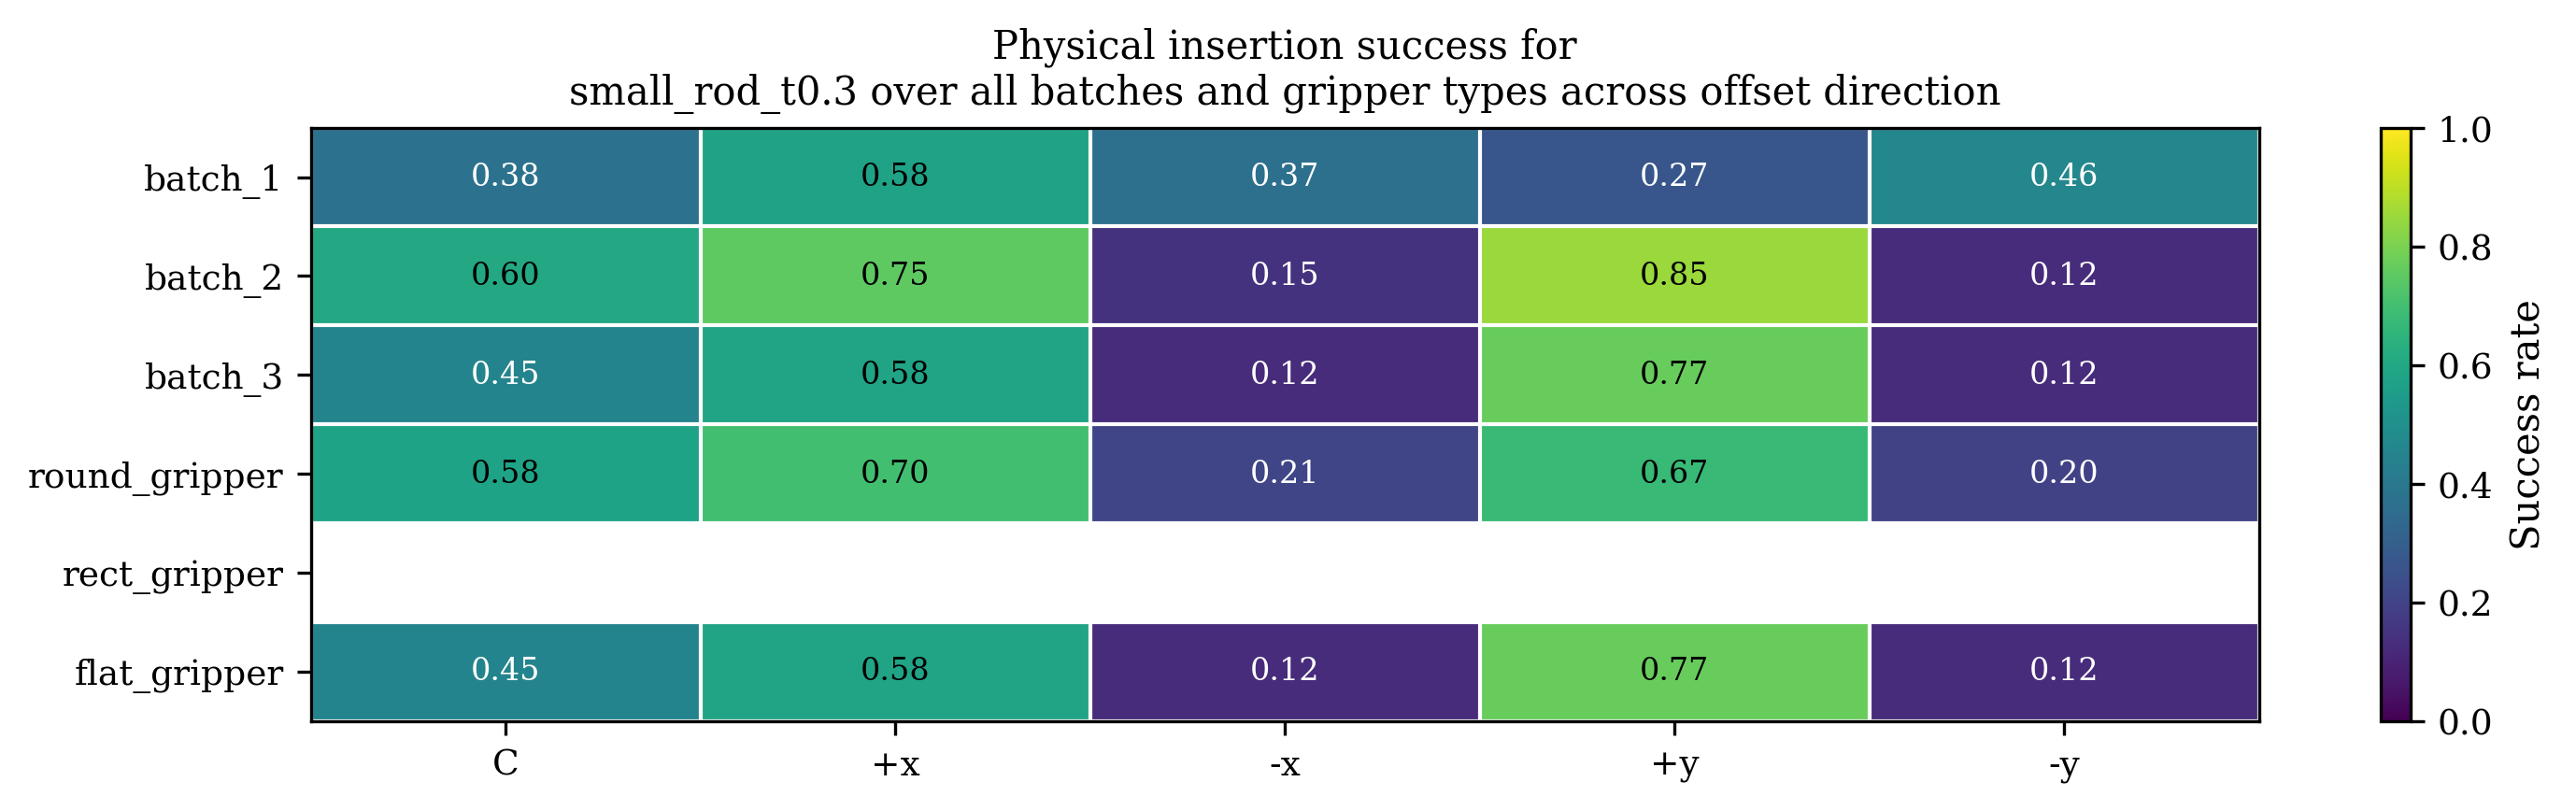
\includegraphics[width=0.95\linewidth]{chapters/7-results_and_discussion/DA1/domain/physical_small_rod_t0.3_batch_gripper_domains_offset_direction.png}
    \caption{Physical success rate of offset-direction groups for \texttt{small\_rod\_t0.3}, separated by batch and gripper domains.}
    \label{fig:da1_small_rod_t03_offset_direction_batch}
\end{figure}

The offset-direction result for \texttt{small\_rod\_t0.3} is investigated in more detail in \figref{fig:da1_small_rod_t03_offset_direction_batch}. The first recorded \texttt{batch\_1} shows a more uniform distribution of offset directions. This is not the case for the later batches, where the asymmetry becomes apparent. This is consistent with the data collection procedure, where in \texttt{batch\_1}, position and orientation deviations were applied more randomly, which can produce individual outliers but does not repeatedly test the same deviation direction with the same offset magnitude. In \texttt{batch\_2} and \texttt{batch\_3}, the deviation planner generated more structured and repeated deviations, so a systematic positional bias becomes more visible.

The distinction between gripper types must be interpreted carefully here. The \texttt{flat} gripper only occurs in \texttt{batch\_3}, while the \texttt{round} gripper is essentially a weighted average of \texttt{batch\_2} and \texttt{batch\_3}. Therefore, the apparent gripper effect is partly coupled with the batch structure and should not be interpreted independently.

\begin{figure}[htbp]
    \centering
    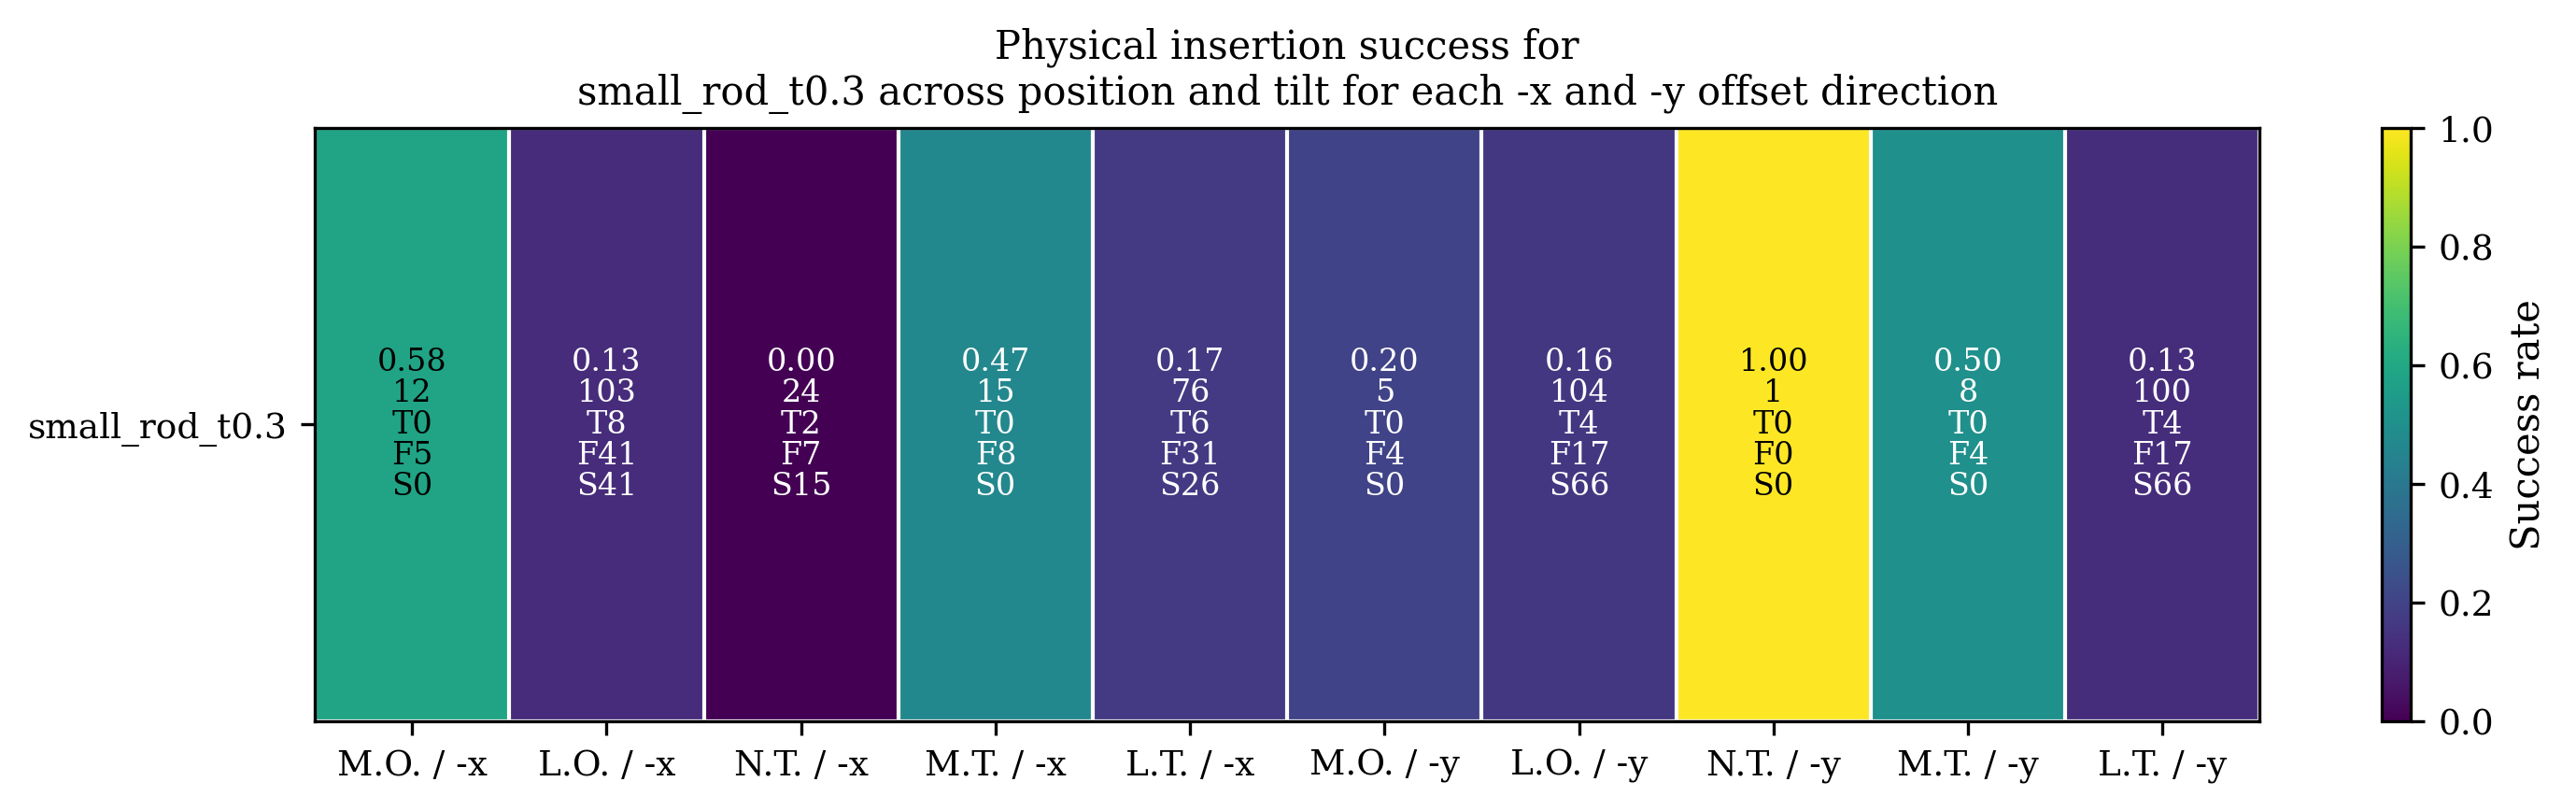
\includegraphics[width=0.95\linewidth]{chapters/7-results_and_discussion/DA1/domain/physical_small_rod_t0.3_domains_offset_direction_3.png}
    \caption{Detailed physical success rate of negative offset directions for \texttt{small\_rod\_t0.3}, separated by offset magnitude and tilt magnitude. Tile annotations include sample counts and failure reasons. N.O. not inlcluded, because the are not associated with a direction, they lie in group \texttt{C}.}
    \label{fig:da1_small_rod_t03_offset_direction_detailed}
\end{figure}

\figref{fig:da1_small_rod_t03_offset_direction_detailed} focuses on the negative $x$ and negative $y$ directions and separates them by offset and tilt magnitude, not combined. Since centered samples are assigned to the centered group \texttt{C}, no-offset cases are not shown for the directional groups. For the negative $x$ direction, the success rate decreases with increasing offset magnitude, which is consistent with the fact that large positional deviations cause make failures more likely. Counterintuitively however, does the no-tilt group in the negative $x$ direction show 0\% success rate. One possible explanation is that, for this specific hole domain and direction, if a tilted rod hits the edge of the hole it can guide itself into the opening, while an untilted rod may hit the top surface of the taskboard more directly and stalls completely. Since for this domain the tolerance is the largest level (\texttt{t0.3}), after a possible self-alignment, the robot can successfully continue the insertion under moderate or large tilt.

The failure-cause annotations support the interpretation that the negative-direction failures are not caused by a single mechanism alone. The failures include force-limit terminations, timeouts, and stall/jam detections. This suggests that the directional bias changes the contact situation in several ways. From a practical perspective, this result is useful, because it suggests a possible correction of the physical insertion setup. Because repeated failures occur mainly for negative $x$ and negative $y$ offsets, the starting pose of an insertion without deviations applied could be shifted slightly in the opposite direction, towards the true hole center, to improve insertion reliability.

\subsubsection{Failure-Cause Analysis for \texttt{rect\_rod\_t0.1}}
\label{subsubsec:da1_rect_rod_t01_force_modes}

\begin{figure}[htbp]
    \centering
    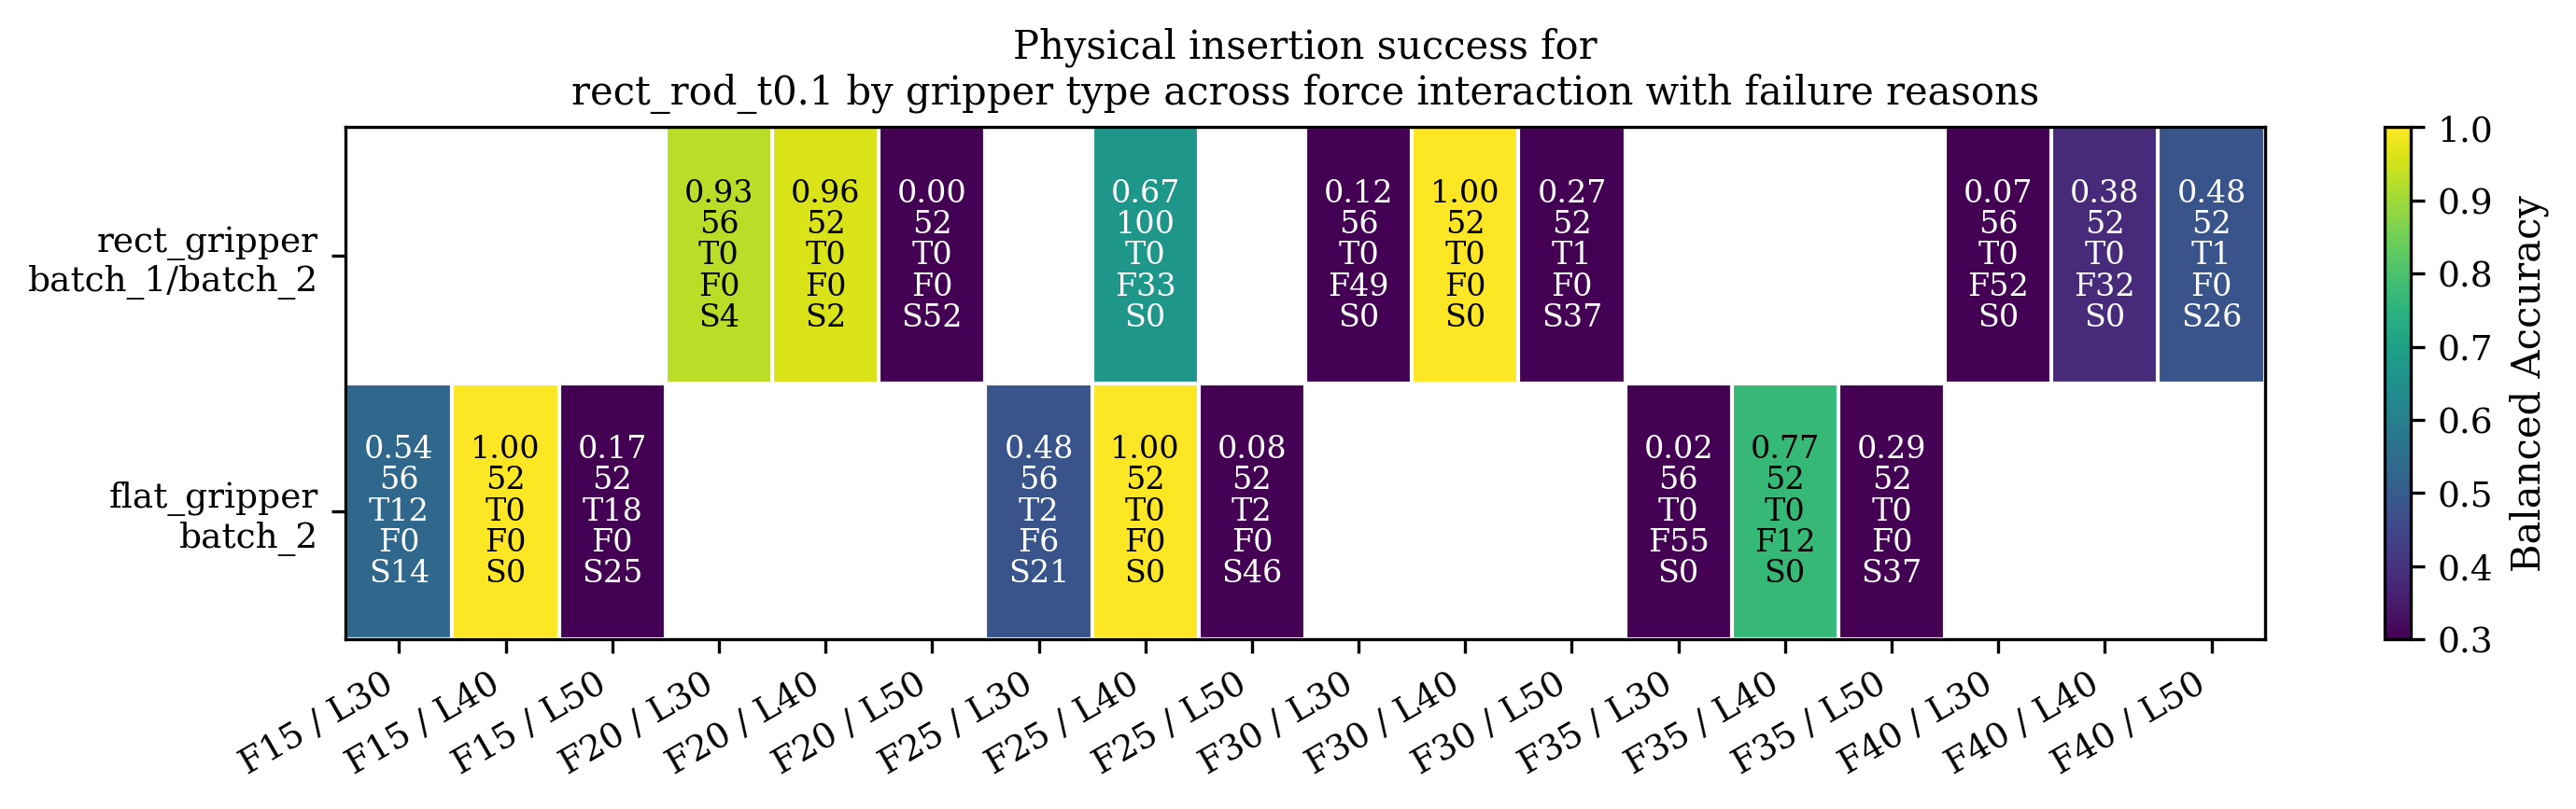
\includegraphics[width=0.95\linewidth]{chapters/7-results_and_discussion/DA1/domain/physical_rect_rod_t0.1_domains_force_interaction_4.png}
    \caption{Detailed physical success rate of force-interaction groups for \texttt{rect\_rod\_t0.1}. Tile annotations include sample counts and failure reasons.}
    \label{fig:da1_rect_rod_t01_force_interaction_failure_modes}
\end{figure}

The hole-domain investigation also identified \texttt{rect\_rod\_t0.1} as an unusual case for the force-interaction groups. This domain is analyzed in more detail in \figref{fig:da1_rect_rod_t01_force_interaction_failure_modes}. The plot separates all insertions from the \texttt{rect\_rod\_t0.1} domain in the \texttt{rect\_gripper} and \texttt{flat\_gripper} domains. This separation also reflects the batch structure, where the rectangular gripper was used in \texttt{batch\_1} and \texttt{batch\_2}, while the flat gripper was exclusively used in \texttt{batch\_3}. Therefore, the observations made, are also gripper- and batch-dependent.

The failure-cause annotations explain the extreme variation seen in the global force-interaction heatmap. Force interactions with a small or negative force difference, such as \texttt{F30/L30}, \texttt{F35/L30}, \texttt{F40/L30}, and \texttt{F40/L40}, fail mainly due to the force limit exceeded. This is expected, because if the insertion force is close to or above the allowed force limit, the insertion is terminate before it can be completed. These cases support the interpretation that the difference between force limit and force level is a deciding factor of whether or not the insertion succeeds.

However, increasing the force limit does not automatically make the insertion successful. Several force interactions with a positive (positive and far from zero) force difference still show low success rates, but their dominant failure cause changes. Instead of force-limit termination, the failures are mainly caused by stall/jam, visible for \texttt{F20/L50}, \texttt{F25/L50}, \texttt{F30/L50} and \texttt{F35/L50}. This indicates that a higher force limit can prevent early timeout termination, but can also allow the system to continue pushing further into a stall or jam. In particular, force limit and stall/jam failure occur in opposite ways, when there are a lot of force limit caused failures, the stall/jam caused failure rate is very low, effectively zero, and vise-versa. The only exception is for \texttt{F25/L30}. Therefore, force-limit failures and stall/jam failures must be interpreted as different physical mechanisms.

Low commanded force levels show another failure mechanism. In some \texttt{F15} cases, a notable number of failures are timeouts. This is consistent with the interpretation that the insertion velocity slows down with lower force levels and the insertion may not finish within the 3s sequence window.

Therefore the force difference is a crucial metric to explain failures caused by force limit versus failures caused by Stall/jam. Especially low forces however can fail because the insertion velocity is too slow, reaching a timeout.

This focused investigation shows why the force-interaction results must be interpreted carefully. The global heatmap correctly identifies force interaction as an important deviation group, but the underlying failure modes and coupled deviations determine whether a low success rate is caused by force-limit termination, timeout, or stall/jam.


\subsubsection{Summary of Deviation Analysis I}
\label{subsubsec:da1_summary}

Deviation Analysis I shows that the physical insertion outcome is strongly dependent on the recorded deviations. The clearest global effect is caused by tilt magnitude. While position offset alone varies on a small scale, the success rate for tilt decreases consistently from no tilt to moderate tilt and large tilt. This trend is also visible in the combined position over tilt groups, where increasing tilt reduces the success rate for each position-offset level. Angular misalignment is therefore more informative for physical insertion difficulty than radial position offset alone.

The second major effect is the interaction between force level and force limit. They cannot be interpreted independently, because the relevant factor is their difference. Settings where the force difference $L-F$ is close to zero or negative show very low success rates, most clearly for \texttt{F40/L30}. In contrast, under favorable geometric conditions without relevant offset or tilt, several force interactions with \texttt{L40} reach complete success. This indicates that unfavorable force settings become especially critical when combined with difficult contact/geometric deviations.

The domain-specific analysis confirms the global tilt trend across most hole domains, but also reveals local effects that are hidden in the global view. In \texttt{small\_rod\_t0.3}, negative $x$ and negative $y$ offsets are significantly less successful than positive offsets, suggesting a directional bias of the start insertion pose without deviations applied. This is practically relevant because such a bias could potentially be corrected by shifting the starting pose in the opposite direction, towards the true hole center.

The investigation of \texttt{rect\_rod\_t0.1} shows that failed insertions come from different physical mechanisms. Low or negative force differences mainly lead to force-limit failures, larger force limits can allow more stall/jam failures, and low force levels can produce timeouts. Therefore, equal success rates do not necessarily represent the same physical behavior. The failure-reason analysis is essential for distinguishing these mechanisms.

Overall, Deviation Analysis I concludes that tilt magnitude and force interaction are the strongest global factors affecting physical success rate, while offset direction can reveal a robotic setup-specific positional bias for selected domains. These results show that the metadata is not only useful for grouping the dataset, but also to explain physically difficult deviations affecting the insertion process.

% MARK: DA2 Model Confusion
\section{Deviation Analysis II: Model Confusion}
\label{sec:results_deviation_analysis_2}

The second part of the deviation analysis evaluates whether specific deviation groups lead to systematic classification errors. The analysis is performed with the PatchTST \texttt{Big} model using the best channel configuration. The model is trained nine times with the same seed combinations used throughout the benchmark experiments. For each run, the mixed data split is 5852 samples for training, 1033 samples for validation and 1215 (659 successful, 556 failed) samples for the test set. Across the nine runs, this produces $1215\times 9 = 10935$ test prediction records.

The plots in this section report the mean and standard deviation of the corresponding metric over the nine runs. This means that the 10935 prediction records are first divided by their queried deviation group, then further divided into nine groups corresponding to the nine training runs, where in each of these groups the model metrics are computed and are averaged. This conceptual split pipeline is visualized in the sankey plot in \figref{fig:da2_sankey}.

The global investigation follows the same deviation groups as Deviation Analysis I. This allows the physical success-rate results to be compared directly with the model-confusion results. The main metric is balanced accuracy, because the deviation groups can have very different success/failure ratios. The binary cross-entropy loss is used as an additional indicator for poor probability estimates, while the false-positive and false-negative rates are used to interpret the direction of the classification errors.

\subsection{Global Screening Across the Mixed Test Set}
\label{subsec:da2_global_screening}

\figref{fig:da2_model_position_tilt_global} and \figref{fig:da2_model_position_over_tilt_global} show the position offset and tilt magnitude side by side and combined, respectively. Here they do not follow the same trend as they did for physical success rate in \figref{fig:da1_physical_position_tilt_global} and \figref{fig:da1_physical_position_over_tilt_global}. In Deviation Analysis I, large tilt was associated with a clear decrease in physical success rate. In the current model-confusion analysis, however, the large-tilt groups still achieve balanced accuracies around 0.86 to 0.90. This indicates that large tilt produces more physical failures, but these failures are often still recognizable from the signal patterns and therefore are not necessarily difficult for the model to classify.

\begin{figure}[htbp]
    \centering
    \begin{minipage}[t]{0.45\textwidth}
        \centering
        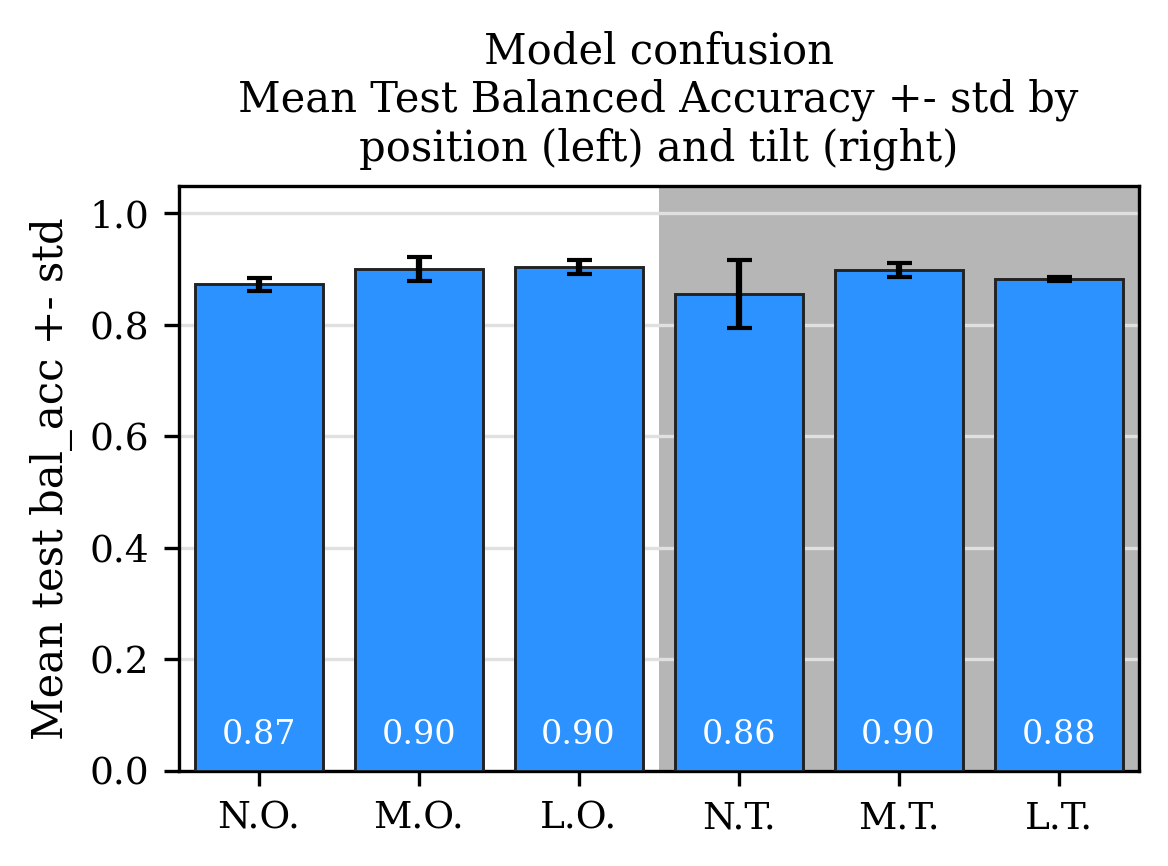
\includegraphics[width=0.95\linewidth]{chapters/7-results_and_discussion/DA2/global/model_position_and_tilt.png}
        \caption{Global model test balanced accuracy for position-offset levels and tilt levels.}
        \label{fig:da2_model_position_tilt_global}
    \end{minipage}
    \hfill
    \begin{minipage}[t]{0.45\textwidth}
        \centering
        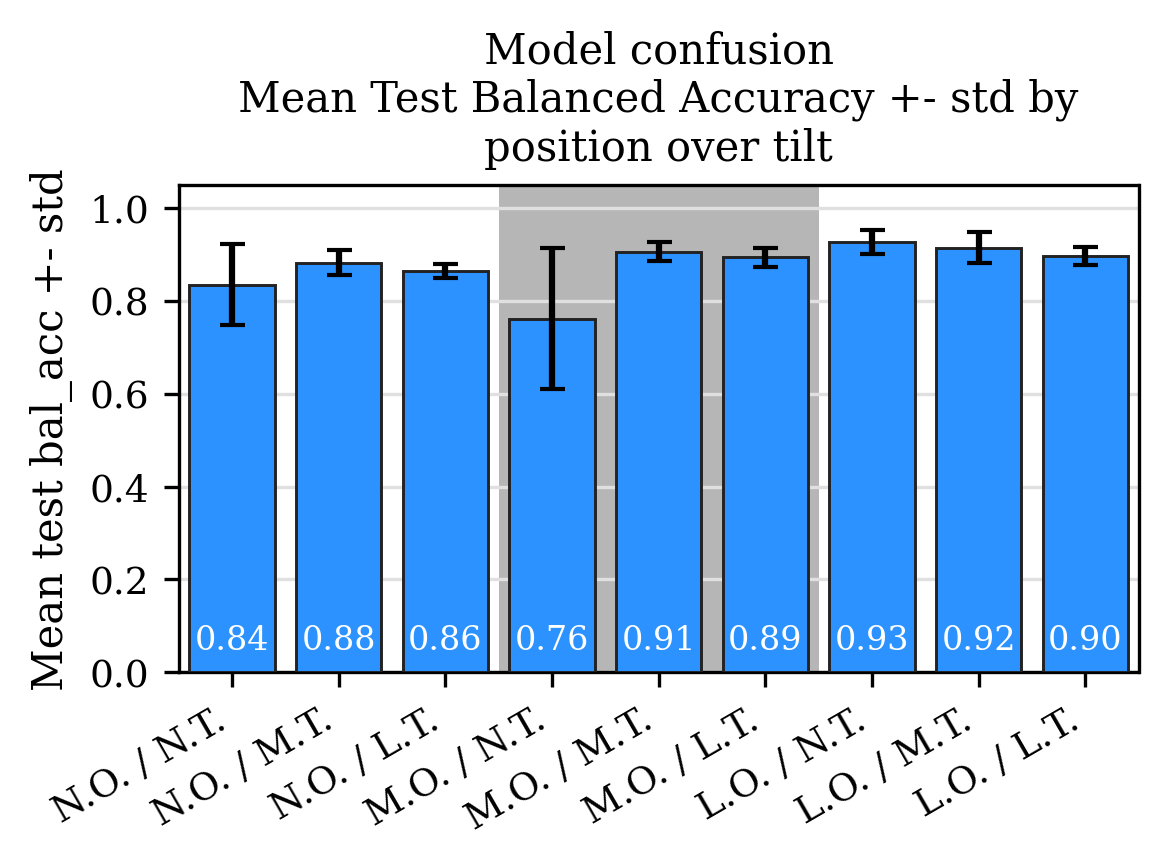
\includegraphics[width=0.95\linewidth]{chapters/7-results_and_discussion/DA2/global/model_position_over_tilt.png}
        \caption{Global model test balanced accuracy for combined position--tilt groups.}
        \label{fig:da2_model_position_over_tilt_global}
    \end{minipage}
\end{figure}

The lowest balanced accuracies within the combined position--tilt groups occur for \texttt{N.O./N.T.} and \texttt{M.O./N.T.}. These groups have really high insertion success rates (\figref{fig:da1_physical_position_over_tilt_global}), but that also means that rare failed insertions in these groups are harder for the model to detect, because of the big class imbalance. This is visible in the false-positive rates listed in \tabref{tab:da2_global_selected_groups}, where \texttt{N.O./N.T.} and \texttt{M.O./N.T.} show comparatively high false-positive rates of around 0.4. In this case, false positive means that a failed insertion is predicted as successful. Thus, the lower balanced accuracy is not caused by generally difficult deviations, but by rare failure cases that are not enough for the model to recognize them.

The offset-direction groups in \figref{fig:da2_model_offset_direction_global} show no strong global model-confusion pattern. While Deviation Analysis I showed that offset direction can reveal domain-specific robotic setup asymmetries, the global model balanced accuracy is relatively uniform across the offset directions. This suggests that offset direction is not a major global source of model confusion.

The force-related results are more informative. \figref{fig:da2_model_force_level_and_limit_global} shows that low and medium force levels, especially \texttt{F15} and \texttt{F25}, are classified with high balanced accuracy, which when comparing with physical success rate in \figref{fig:da1_physical_force_level_and_limit_global} shows the same trend as for the \texttt{N.O./N.T.} and \texttt{M.O./N.T.} cases, only in the opposite direction. Meaning, an unpreferable physical success rate of close to 50\%  provides a favorable class split for the model to train on.

\begin{figure}[htbp]
    \centering
    \begin{minipage}[t]{0.45\textwidth}
        \centering
        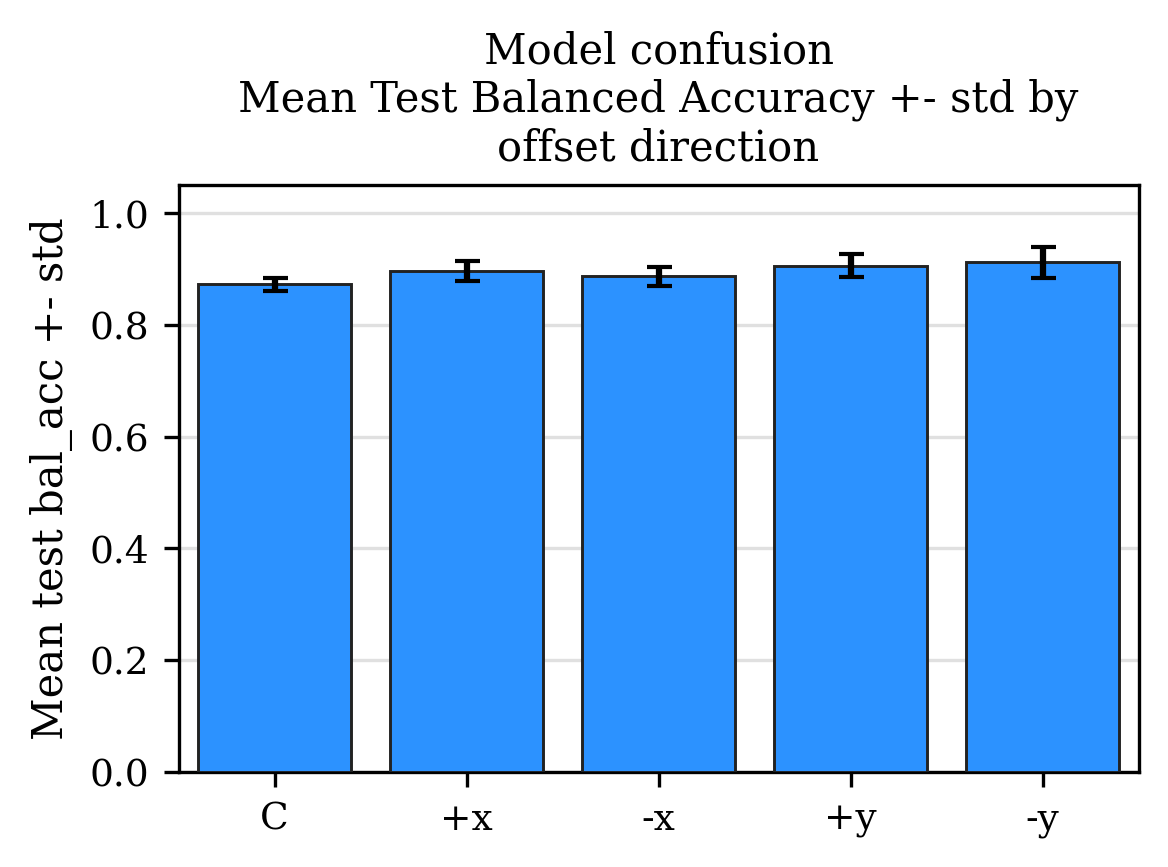
\includegraphics[width=0.9\linewidth]{chapters/7-results_and_discussion/DA2/global/model_offset_direction.png}
        \caption{Global model test balanced accuracy for offset-direction groups.}
        \label{fig:da2_model_offset_direction_global}
    \end{minipage}
    \hfill
    \begin{minipage}[t]{0.45\textwidth}
        \centering
        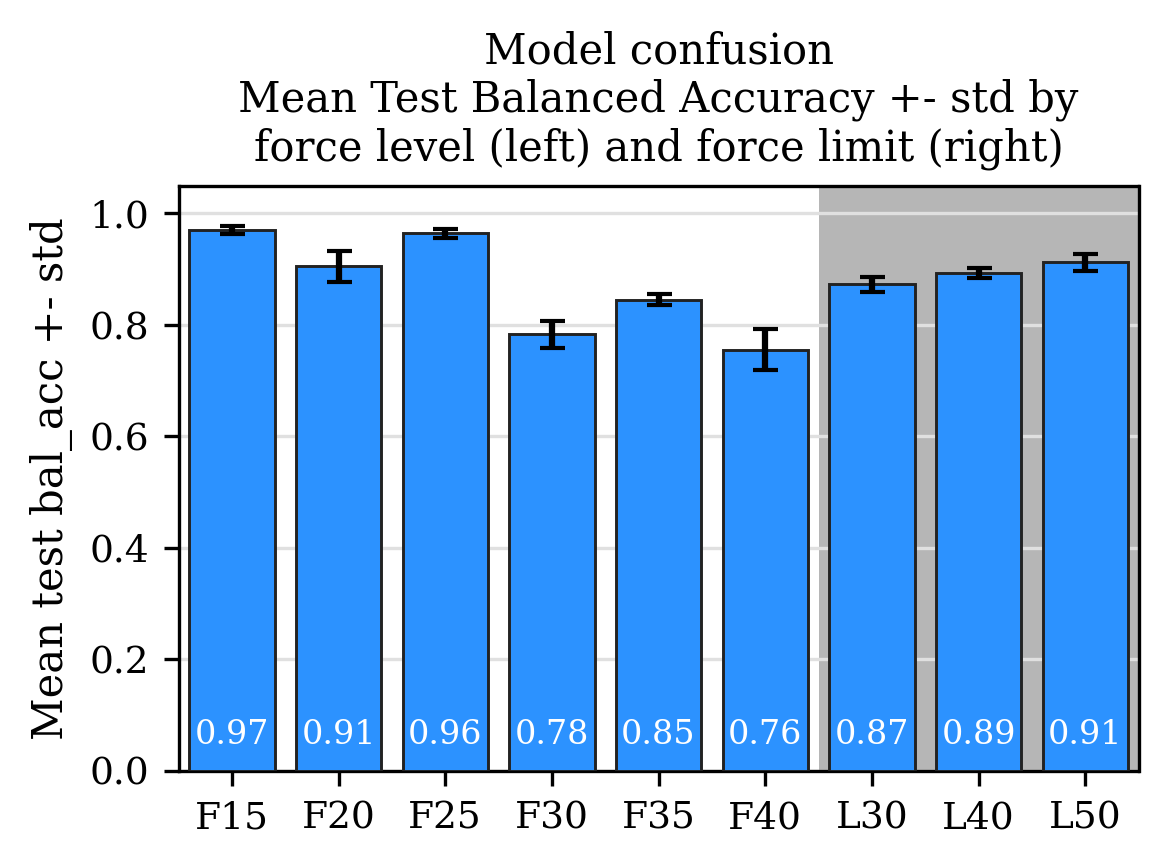
\includegraphics[width=0.9\linewidth]{chapters/7-results_and_discussion/DA2/global/model_force_level_and_limit.png}
        \caption{Global model balanced accuracy for force level and force limit.}
        \label{fig:da2_model_force_level_and_limit_global}
    \end{minipage}
\end{figure}

The force limit alone is less informative, because the effect depends on the commanded force level. Therefore, the force-interaction groups in \figref{fig:da2_model_force_interaction_global} and \figref{fig:da2_model_loss_force_interaction_global} provide the clearest view. The lowest balanced accuracy occurs for \texttt{F40/L30}, with $0.467 \pm 0.019$. This group is physically almost always a failure, with only 15 successful insertions among 543 prediction records. The false-negative rate is 1.0, meaning that all rare successful insertions in this group are predicted as failures.
This does not mean that the model fails to recognize the dominant failures \texttt{F40/L30}. The opposite is the case, where the few successful exceptions are not recognized by the model. This is a case where the group is physically very difficult and where the class distribution itself makes the rare positive class hard to identify.

\begin{figure}[htbp]
    \centering
    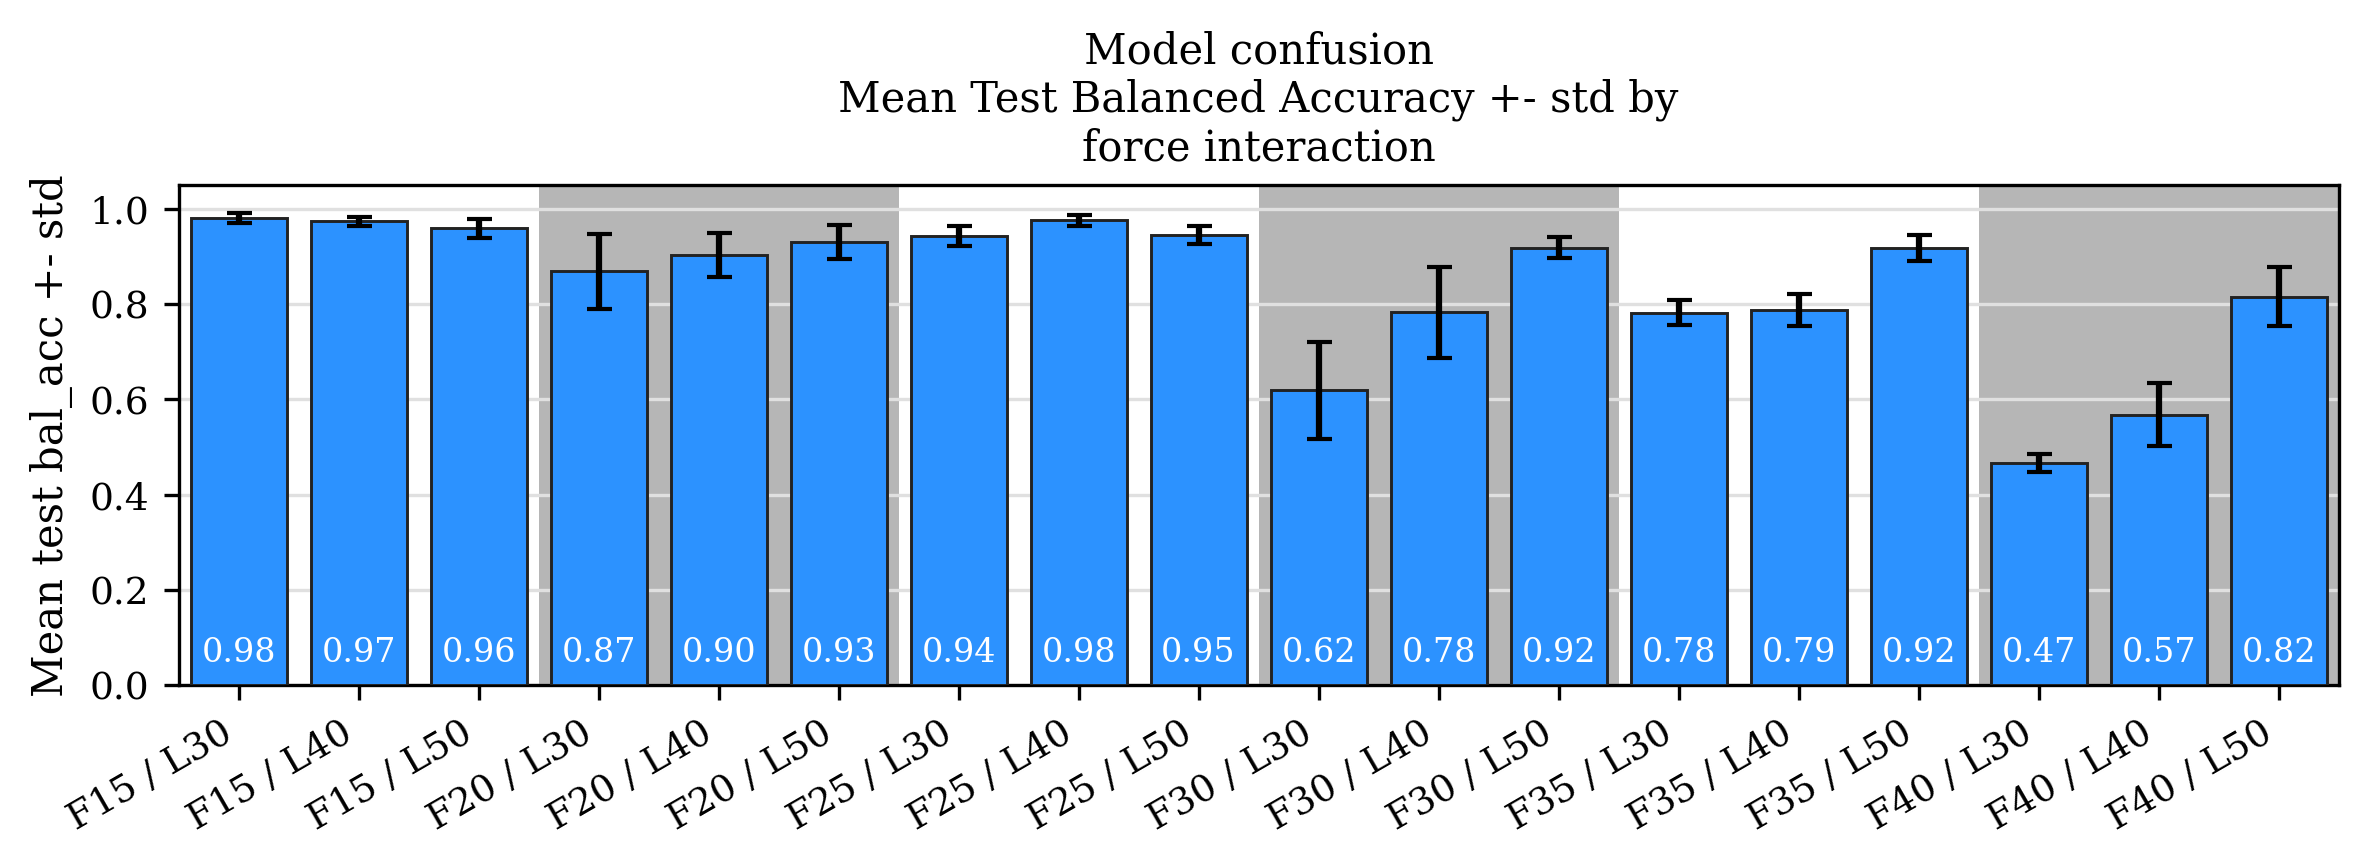
\includegraphics[width=0.9\linewidth]{chapters/7-results_and_discussion/DA2/global/model_force_interaction.png}
    \caption{Global model test balanced accuracy for force-interaction groups.}
    \label{fig:da2_model_force_interaction_global}
\end{figure}

\begin{figure}[htbp]
    \centering
    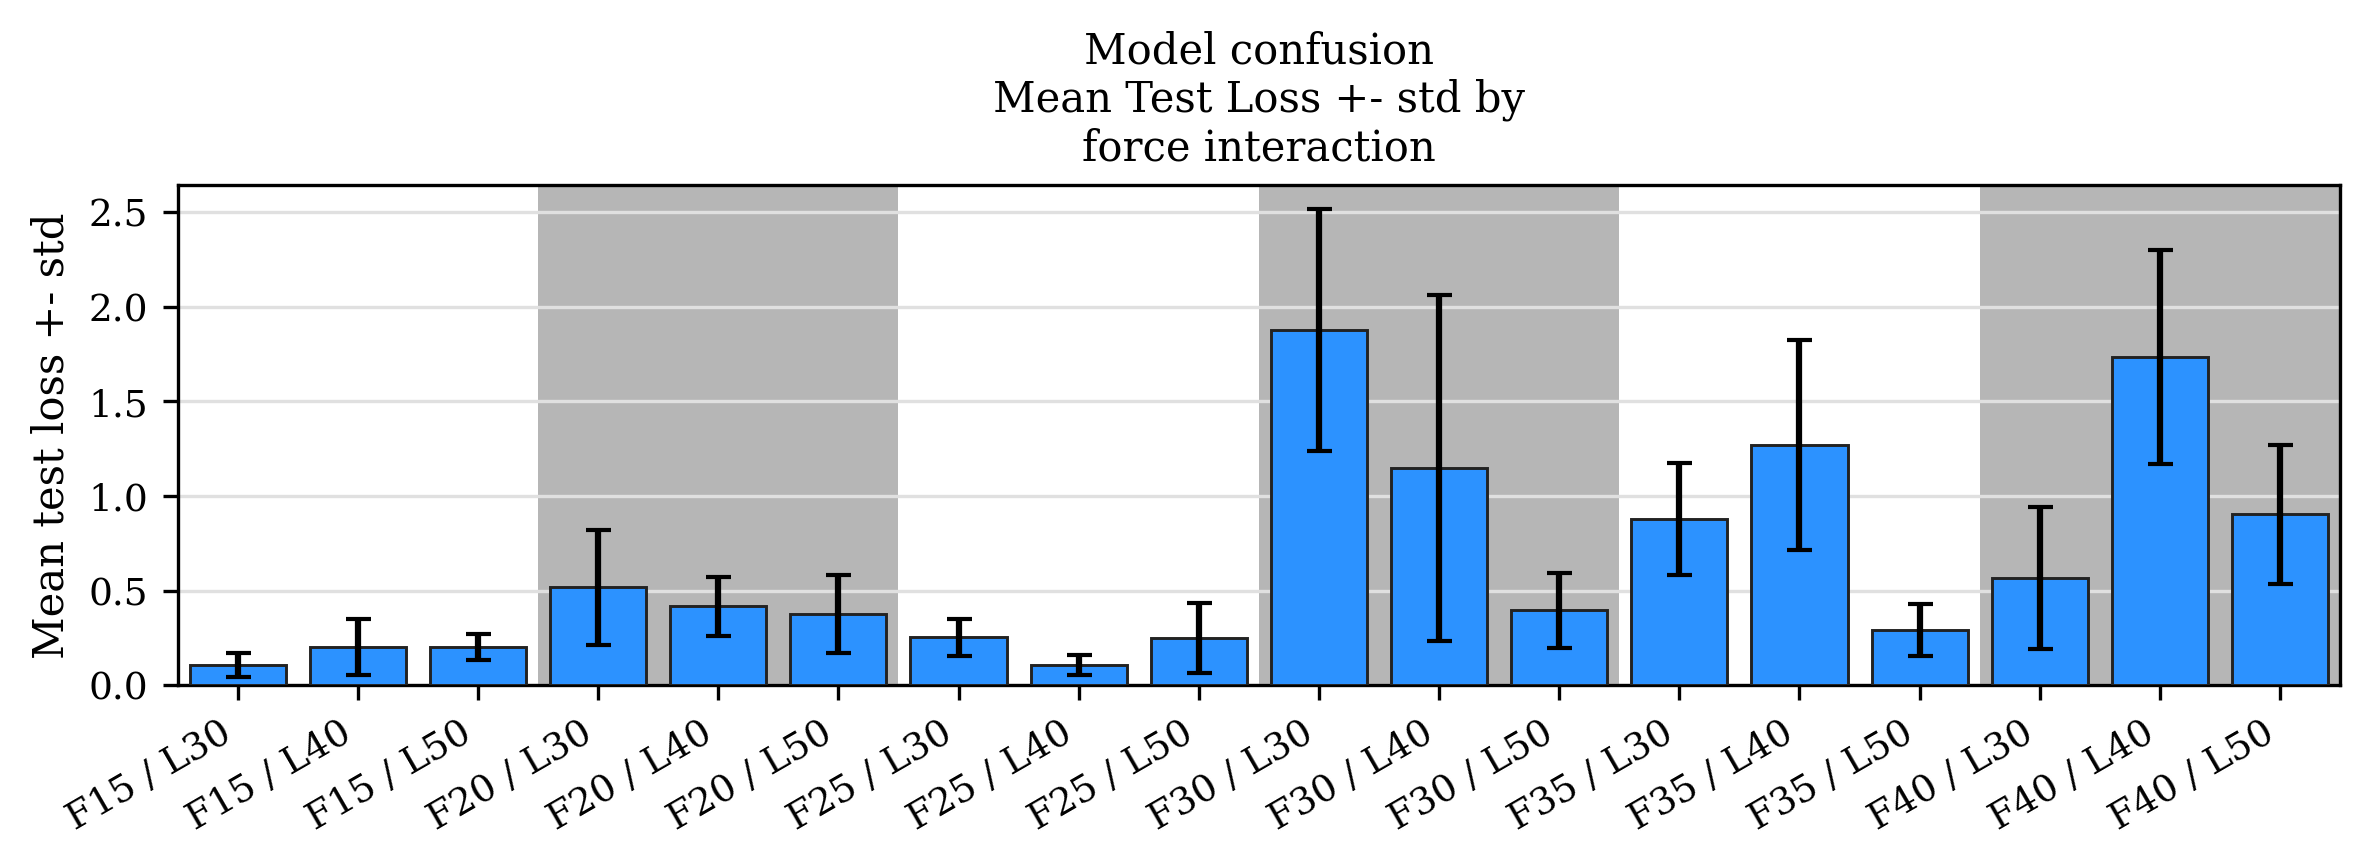
\includegraphics[width=0.9\linewidth]{chapters/7-results_and_discussion/DA2/global/model_loss_force_interaction.png}
    \caption{Global binary cross-entropy loss for force-interaction groups.}
    \label{fig:da2_model_loss_force_interaction_global}
\end{figure}

In an unbalanced case like this, it is really beneficial to report the balanced accuracy, because accuracy alone does not compensate for the high class imbalance.
In this specific case the confusion matrix is $\text{TP} = 0, \text{TN} = 493, \text{FP} = 35, \text{FN} = 15$, which according to the formulas in \tabref{tab:classification_metrics} computes a balanced accuracy of 0.467 and accuracy of 0.908, which is huge difference.

Other force-interaction groups show a different kind of model confusion. In particular, \texttt{F30/L30} and \texttt{F40/L40} have both low balanced accuracy and the highest binary cross-entropy losses. The group \texttt{F30/L30} reaches only $0.619 \pm 0.102$ balanced accuracy with a loss of $1.878 \pm 0.640$, while \texttt{F40/L40} reaches $0.568 \pm 0.066$ balanced accuracy with a loss of $1.735 \pm 0.566$. A high loss means that the model often assigns high confidence to the wrong class, or gives low probability to the true class, which is penalized more strongly than an uncertain prediction near the decision boundary. Thus, the issue is not only that some samples fall on the wrong side of the threshold, but that the predicted probabilities themselves are mostly wrong. This indicates genuinely ambiguous or inconsistent signal patterns for the model.

Within several force levels, increasing the force limit improves the model performance. For example, the balanced accuracy increases from \texttt{F30/L30} to \texttt{F30/L50}, and from \texttt{F40/L30} to \texttt{F40/L50}. This is consistent with the interpretation from Deviation Analysis I: when the commanded force is close to or above the force limit, the insertion behavior is dominated by early termination (force limit reached) or unusual contact dynamics. This produces signal patterns that are less consistent for the classifier.

The record-offset groups in \figref{fig:da2_model_record_offset_global} are very uniform. The early-offset group (\texttt{ROE}) has the highest balanced accuracy, but the mid (\texttt{ROM}), and late (\texttt{ROL}) groups remain in a similar range. This suggests that the classifier is not strongly dependent on one exact temporal recording-window position. Since record offset is not a physical insertion deviation, this is mainly a model-side result: the tested recording-window shifts do not create a severe global model-confusion effect.

Finally, \figref{fig:da2_model_grasp_approach_height_global} shows that approach height 0 mm (\texttt{AH0}) reaches a very high balanced accuracy of $0.985 \pm 0.008$. This result should be interpreted carefully, because batch 1 was exclusively recorded with approach height 0 mm and grasp height 0 mm as well. It is therefore not interpreted as an isolated effect of approach height. Instead, it is treated as a candidate for domain-specific inspection if required.


\begin{figure}[htbp]
    \centering
    \begin{minipage}[b]{0.45\textwidth}
        \centering
        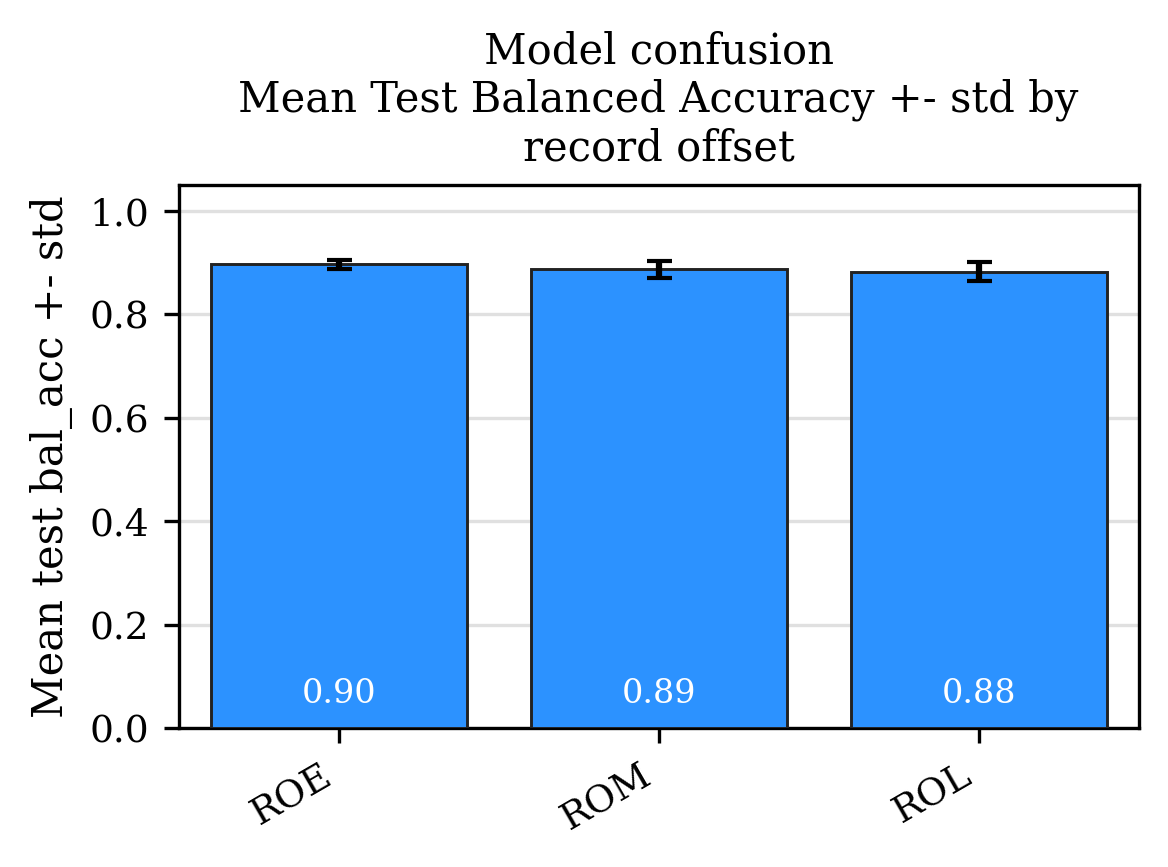
\includegraphics[width=0.9\linewidth]{chapters/7-results_and_discussion/DA2/global/model_record_offset.png}
        \caption{Global model test balanced accuracy for record-offset groups.}
        \label{fig:da2_model_record_offset_global}
    % \end{minipage}
        \vspace{3.0cm}
    % \begin{minipage}[t]{0.45\textwidth}
        % \centering
        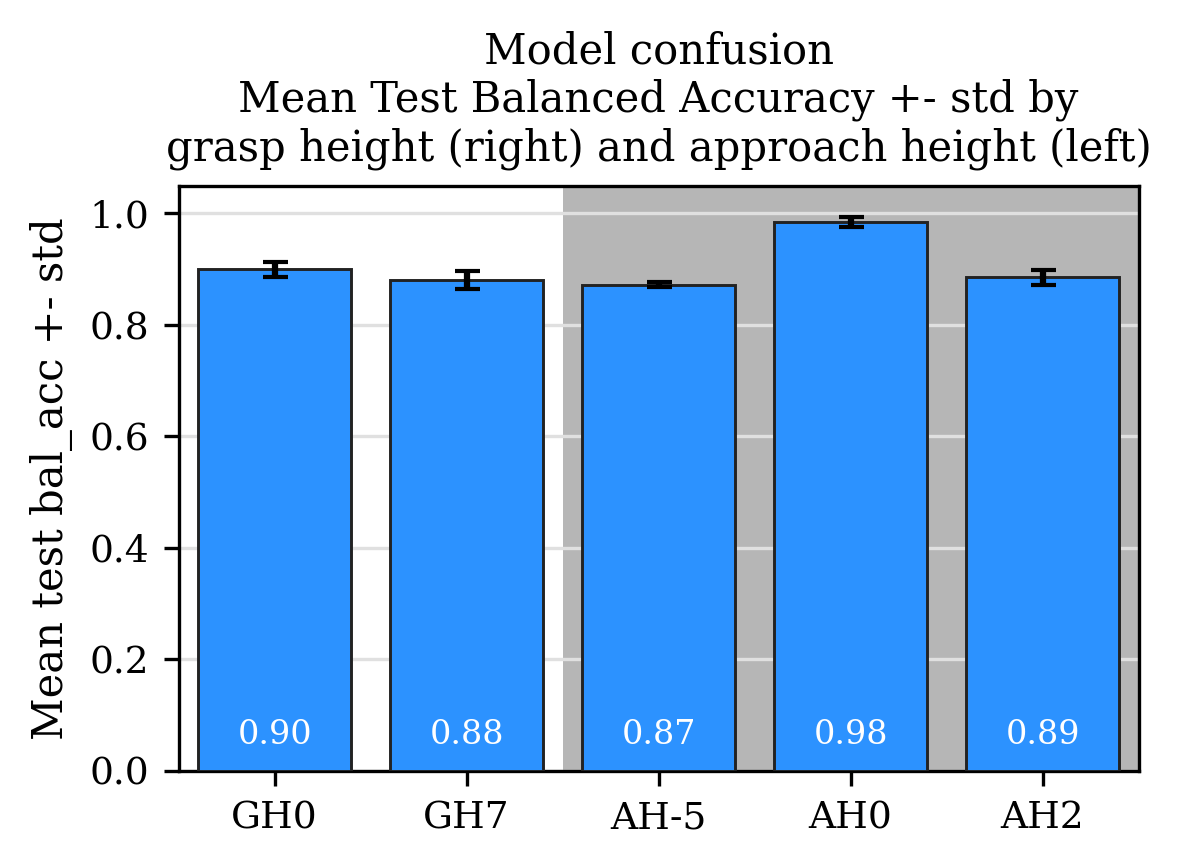
\includegraphics[width=0.9\linewidth]{chapters/7-results_and_discussion/DA2/global/model_grasp_approach_height.png}
        \caption{Global model test balanced accuracy for grasp-height and approach-height groups.}
        \label{fig:da2_model_grasp_approach_height_global}
    \end{minipage}
    \hfill
    \begin{minipage}[b]{0.45\textwidth}
        \centering
        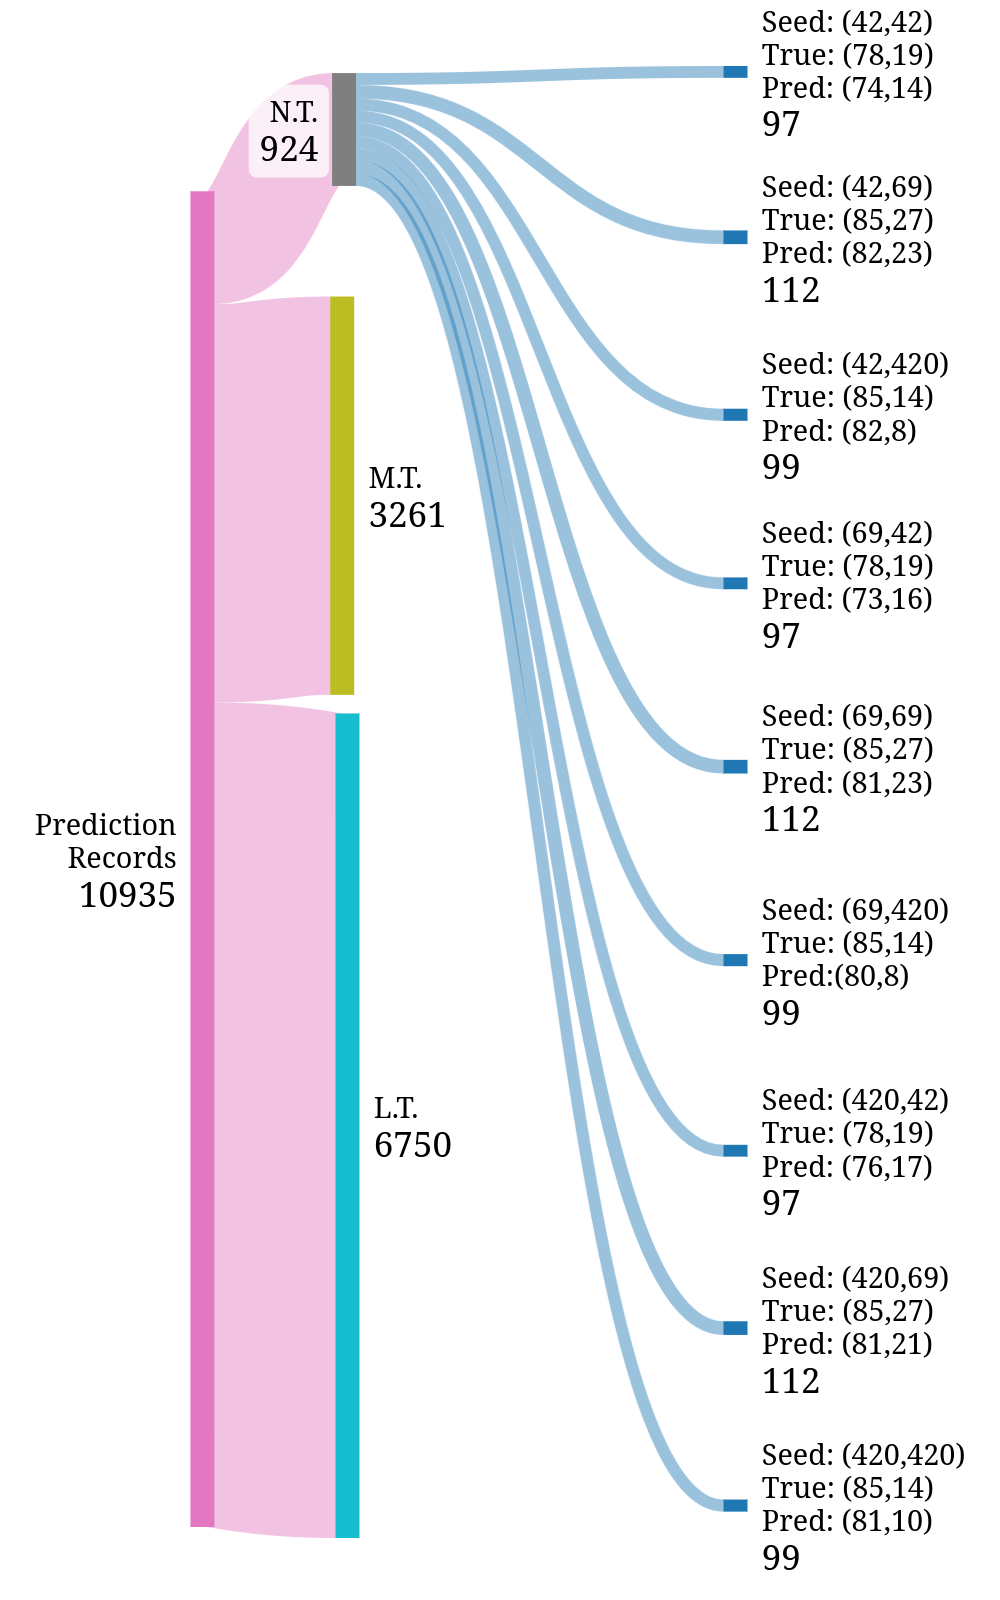
\includegraphics[width=0.9\linewidth]{chapters/7-results_and_discussion/DA2/global/sankey.png}
        \caption{Sankey plot of the splitting pipeline to compute the queried mean metric. First all prediction records get split into the queried deviation groups, which each containing the predictions among the 9 training runs. Inside the seed groups the metrics: Balanced Accuracy, BCE Loss, False Positive Rate and False Negative Rate are computed. The visualized pattern is: "Seed:(model seed, split seed), True:(\#successful insertions, \#failed insertions), Pred:(TP, TN)". TP and TN come from the confusion matrix, FP, FN are not listed.}
        \label{fig:da2_sankey}
    \end{minipage}
\end{figure}

\begin{table}[htbp]
    \centering
    \caption{Selected global model-confusion results. The sample counts and class splits are accumulated across all nine test evaluations. The "Pred." Prediction entry defines pos = TP + TN, neg = FP + FN.}
    \label{tab:da2_global_selected_groups}
    \scriptsize
    \begin{adjustbox}{width=\textwidth}
    \begin{tabular}{lllllllll}
        \toprule
        \textbf{Deviation Group} &
        \textbf{\#} &
        \textbf{True (pos, neg)} &
        \textbf{Pred. (pos, neg)} &
        \textbf{Bal. acc.} &
        \textbf{Loss} &
        \textbf{FPR} &
        \textbf{FNR} \\
        \midrule
        \texttt{position\_tilt}\\
        \texttt{N.O./N.T.} & 267 & (237, 30) & (246, 21) & 0.835 $\pm$ 0.088 & 0.461 & 0.389 & 0.045 \\
        \texttt{M.O./N.T.} & 378 & (321, 57) & (340,38) & 0.762 $\pm$ 0.152 & 0.599 & 0.417 & 0.060 \\
        \texttt{N.O./L.T.} & 2781 & (1317, 1464) & (2402,379) & 0.864 $\pm$ 0.015 & 0.682 & 0.133 & 0.139 \\
        \texttt{M.O./L.T.} & 1653 & (744, 909) & (1480,173) & 0.894 $\pm$ 0.021 & 0.576 & 0.093 & 0.118 \\
        \texttt{L.O./L.T.} & 2316 & (1122, 1194) & (2080,236) & 0.897 $\pm$ 0.020 & 0.470 & 0.082 & 0.124 \\
        \midrule
        \texttt{force\_interaction} \\
        \texttt{F15/L30} & 588 & (363, 225) & (576,12) & 0.980 $\pm$ 0.010 & 0.108 & 0.020 & 0.019 \\
        \texttt{F15/L40} & 489 & (351, 138) & (472,17) & 0.974 $\pm$ 0.009 & 0.203 & 0.007 & 0.046 \\
        \texttt{F25/L40} & 1842 & (1089, 753) & (1800,42) & 0.976 $\pm$ 0.011 & 0.106 & 0.032 & 0.016 \\
        \texttt{F30/L30} & 564 & (111, 453) & (368,196) & 0.619 $\pm$ 0.102 & 1.878 & 0.323 & 0.439 \\
        \texttt{F30/L40} & 576 & (513, 63) & (463,113) & 0.783 $\pm$ 0.096 & 1.148 & 0.238 & 0.196 \\
        \texttt{F30/L50} & 594 & (414, 180) & (535,59) & 0.918 $\pm$ 0.022 & 0.395 & 0.041 & 0.123 \\
        \texttt{F35/L40} & 498 & (309, 189) & (396,102) & 0.788 $\pm$ 0.034 & 1.270 & 0.245 & 0.178 \\
        \texttt{F40/L30} & 543 & (15, 528) & (493,50) & 0.467 $\pm$ 0.019 & 0.568 & 0.067 & 1.000 \\
        \texttt{F40/L40} & 537 & (84, 453) & (385,152) & 0.568 $\pm$ 0.066 & 1.735 & 0.211 & 0.653 \\
        \texttt{F40/L50} & 507 & (366, 141) & (395,112) & 0.815 $\pm$ 0.062 & 0.902 & 0.106 & 0.263 \\
        \midrule
        \texttt{record\_offset} \\
        \texttt{ROE} & 5193 & (2721, 2472) & (4657, 536) & 0.897 $\pm$ 0.009 & 0.556 & 0.0959 & 0.110 \\
        \texttt{ROM} & 1797 & (996, 801) & (975, 822) & 0.887 $\pm$ 0.017 & 0.527 & 0.112 & 0.113 \\
        \texttt{ROE} & 3945 & (2214, 1731) & (2200, 1745) & 0.883 $\pm$ 0.018 & 0.623 & 0.129 & 0.106 \\
        \midrule
        \texttt{approach\_height} \\
        \texttt{AH0} & 1284 & (705, 579) & (1265, 19) & 0.985 $\pm$ 0.008 & 0.081 & 0.022 & 0.008 \\
        \bottomrule
    \end{tabular}
    \end{adjustbox}
\end{table}


Overall, the global model confusion analysis shows that the final model using the best channels is comparatively robust across most geometric deviation groups. This differs from the physical success-rate analysis, where large tilt clearly caused more insertion failures. The main global model confusion patterns are instead found in force interaction groups. In particular, force settings with a small or negative difference between force limit and force level produce either rare successful exceptions that are missed by the model, as in \texttt{F40/L30}, or genuinely ambiguous signal patterns, as in \texttt{F30/L30} and \texttt{F40/L40} are difficult to classify. Furthermore some cases showed consistent patterns between physical success rate and balanced accuracy, where a success rate close to 50\%, inherently means a fairly balanced class split, which is favorable for the model to train on. On the other hand a physically favorable insertion success rates of around 100\%, or the other unfavorable extreme case of around 0\% success rate, inherently causes class imbalance that in turn biases the model to one extreme case.

The record-offset groups do not show a severe performance collapse, indicating that the model is reasonably robust to the tested temporal recording-window shifts.

% MARK: DA2 Domain
\subsection{Domain-Specific Follow-Up Analysis}
\label{subsec:da2_domain_specific}

The global model-confusion analysis showed that most geometric deviation groups are classified comparatively robustly, while significant model-confusion patterns occur in force-interaction groups. The domain-specific follow-up analysis therefore focuses on two questions. First, it investigates whether the force-interaction model confusion is distributed across domains or caused by individual hole configurations. Second, it checks whether local effects found in Deviation Analysis I, such as the directional bias in \texttt{small\_rod\_t0.3}, also appear as model-confusion effects.

For this analysis, the heatmap annotations are extended in selected plots. In addition to the balanced accuracy, the true class split are shown for each tile in the following format: (true number of successes, true number of fails). Furthermore, the confusion-matrix entries are reported in the form \texttt{TP}, \texttt{TN}, \texttt{FP}, and \texttt{FN}. This makes it possible to distinguish whether a low balanced accuracy is caused by many false positives, many false negatives, or simply by a very small number of samples.

\subsubsection{Force Interaction Across Hole Domains}
\label{subsubsec:da2_force_interaction_domains}

\figref{fig:da2_domain_force_interaction_holes} shows the model test balanced accuracy for the force-interaction groups across the hole domains. The result is consistent with the global analysis: force interactions with a small or negative force difference remain among the most difficult cases for the model. In particular, settings such as \texttt{F30/L30}, \texttt{F35/L30}, and \texttt{F40/L40} show reduced balanced accuracy in several domains.

At the same time, the heatmap shows that the confusion is not uniform across all hole domains. Some force-interaction settings are classified well in one hole domain (\texttt{big\_rod\_t0.3} and \texttt{rect\_rod\_t0.2}) but poorly in another (\texttt{small\_rod\_t0.1}, \texttt{rect\_rod\_t0.1} and \texttt{rect\_rod\_t0.3}). This indicates that the force interaction cannot be interpreted independently from the geometric hole configurations. However, the overall pattern still supports the global conclusion that the model-confusion effects are strongest when the commanded insertion force is close to or above the force limit.

\begin{figure}[htbp]
    \centering
    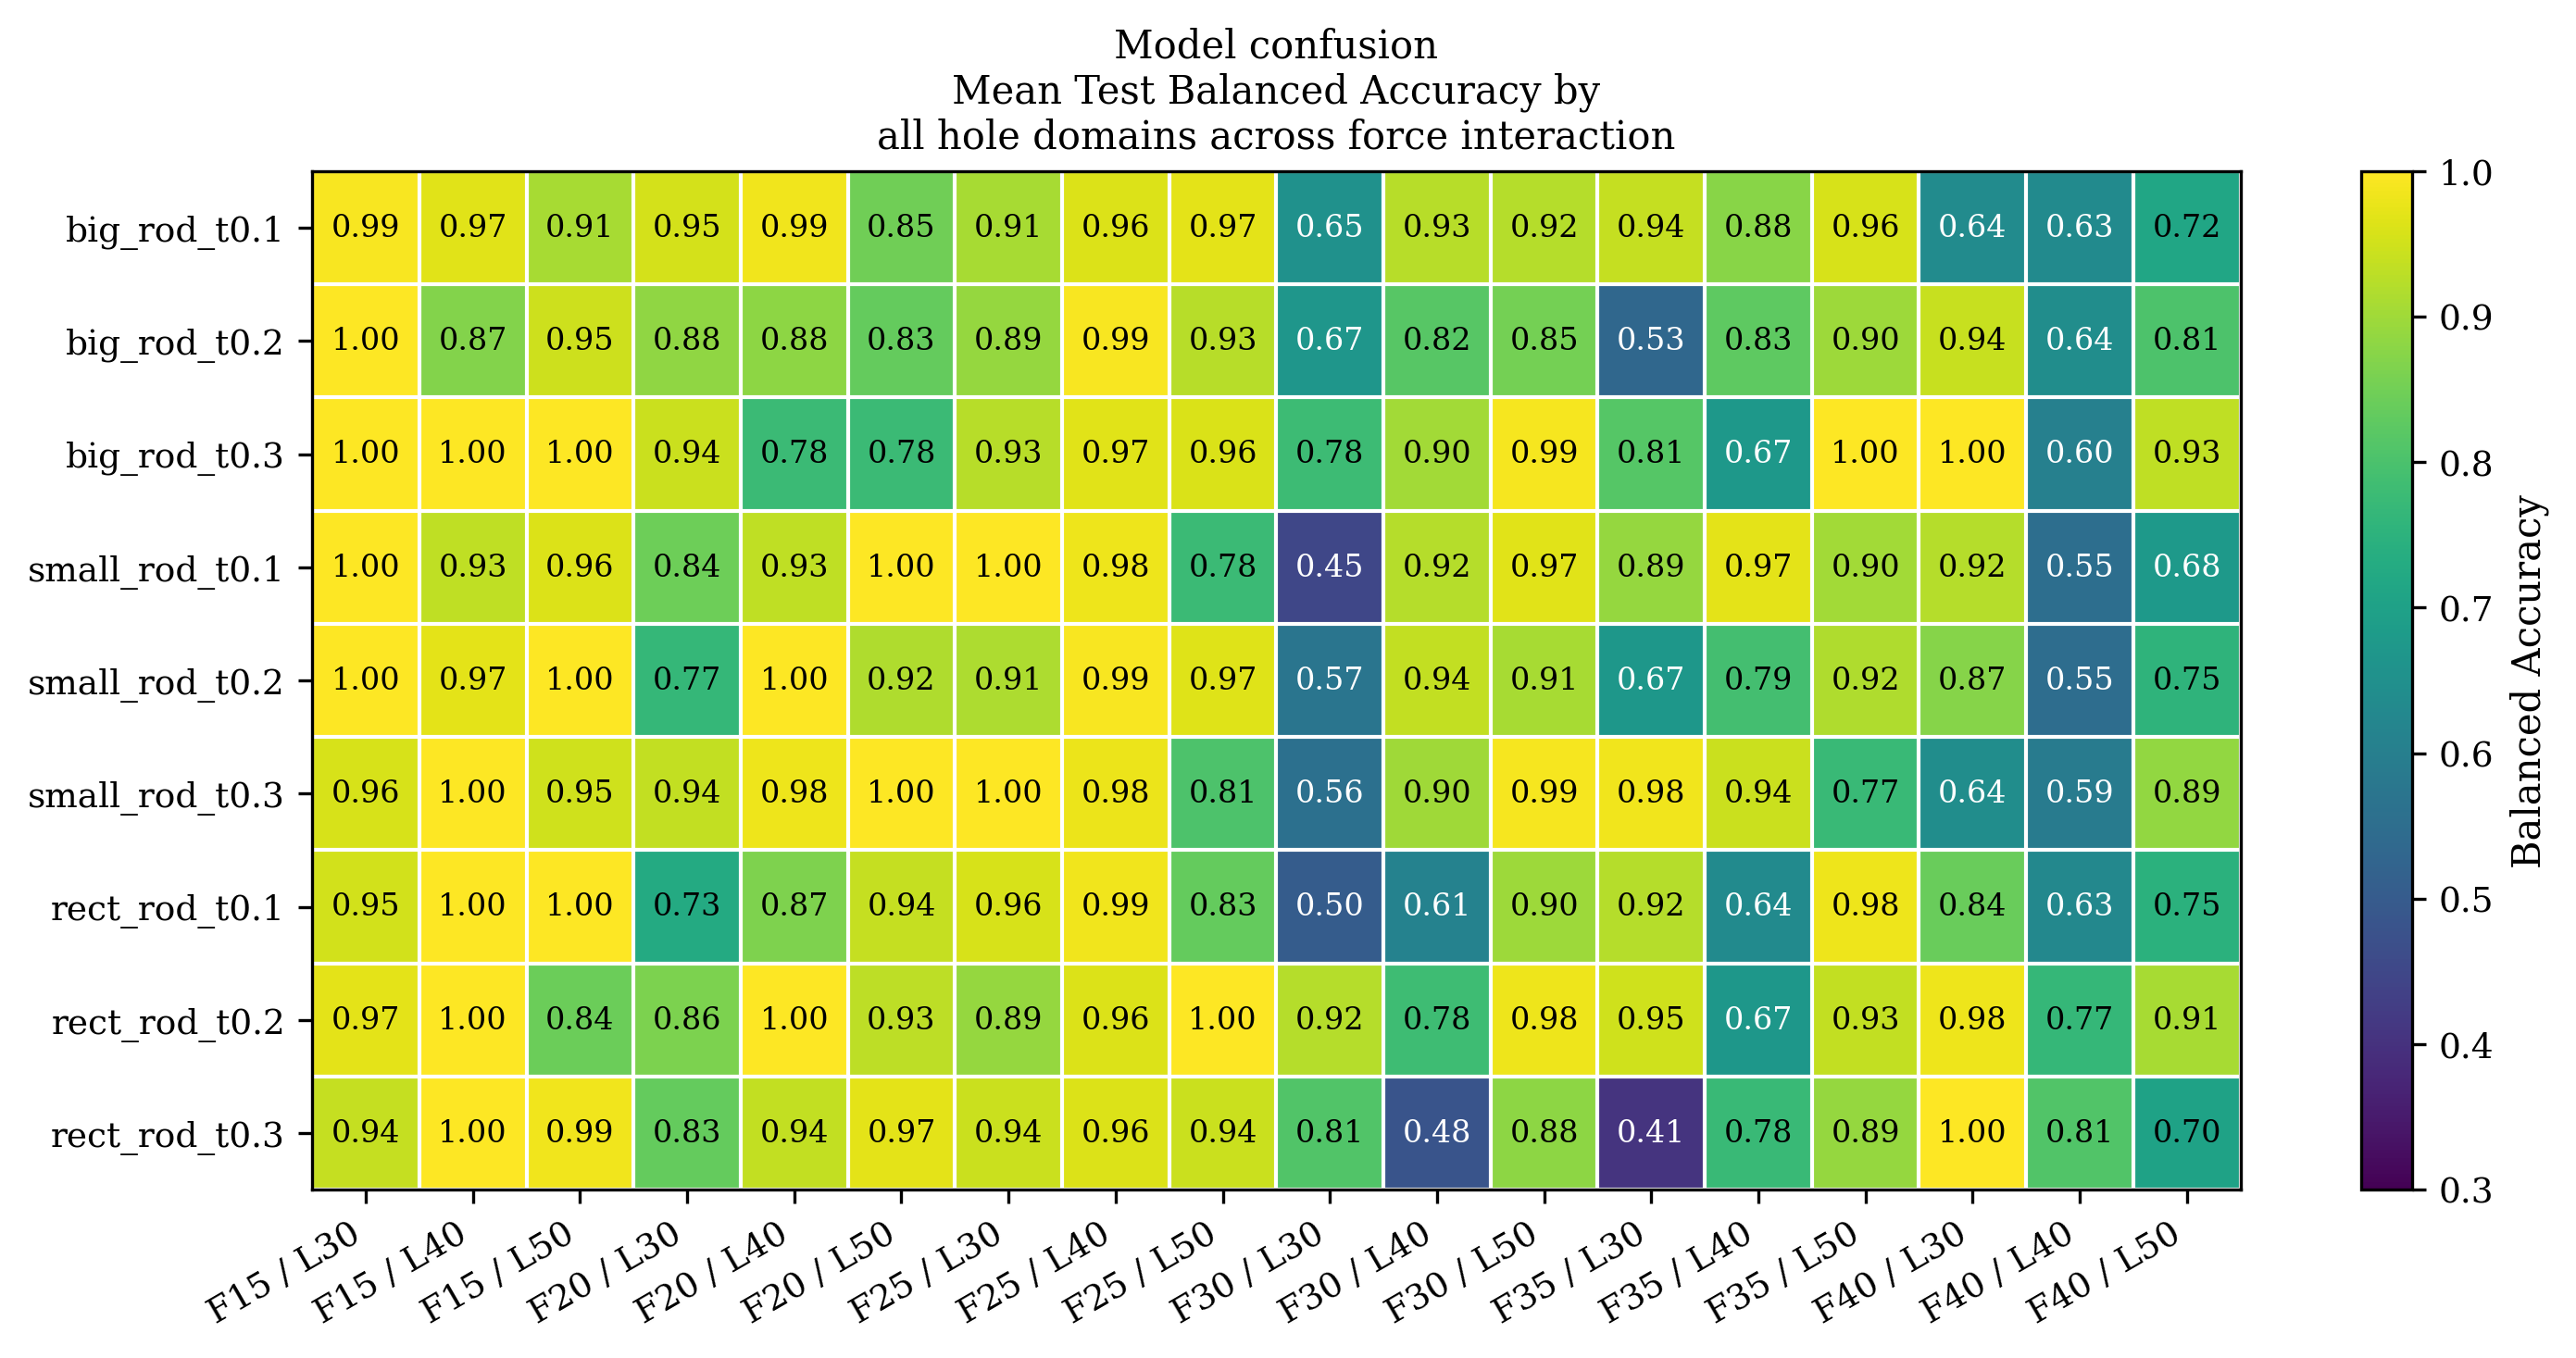
\includegraphics[width=0.95\linewidth]{chapters/7-results_and_discussion/DA2/domain/model_hole_domain_force_interaction.png}
    \caption{Domain-specific model balanced accuracy for force-interaction groups across hole domains.}
    \label{fig:da2_domain_force_interaction_holes}
\end{figure}

\subsubsection{Detailed Inspection of \texttt{F30/L30}}
\label{subsubsec:da2_f30_l30}

The force-interaction group \texttt{F30/L30} is inspected in more detail in \figref{fig:da2_position_tilt_f30_l30}. This group was selected because it shows both reduced balanced accuracy and high loss in the global analysis (\figref{fig:da2_model_force_interaction_global} and \figref{fig:da2_model_loss_force_interaction_global}). The figure queries the whole dataset for the \texttt{F30/L30} group and splits it further in the nine position over tilt groups. It indicates that the low performance is not caused by one isolated position--tilt group. Instead, several available position--tilt combinations show reduced balanced accuracy.

The confusion-matrix annotations show that both false positives and false negatives occur. Therefore, the model does not simply predict one class for the entire group, but has difficulty separating successful and failed insertions within this force interaction group. Since the corresponding failed insertions are dominated by force-limit terminations, as shown in \figref{fig:da2_position_tilt_f30_l30_failure_reason}, the ambiguity is likely related to the sudden force limit stopping behavior, that doesnt provide information rich signal patterns to justify this fail. This supports the interpretation that \texttt{F30/L30} is a genuinely ambiguous force-interaction group for the model.

\begin{figure}[htbp]
    \centering
    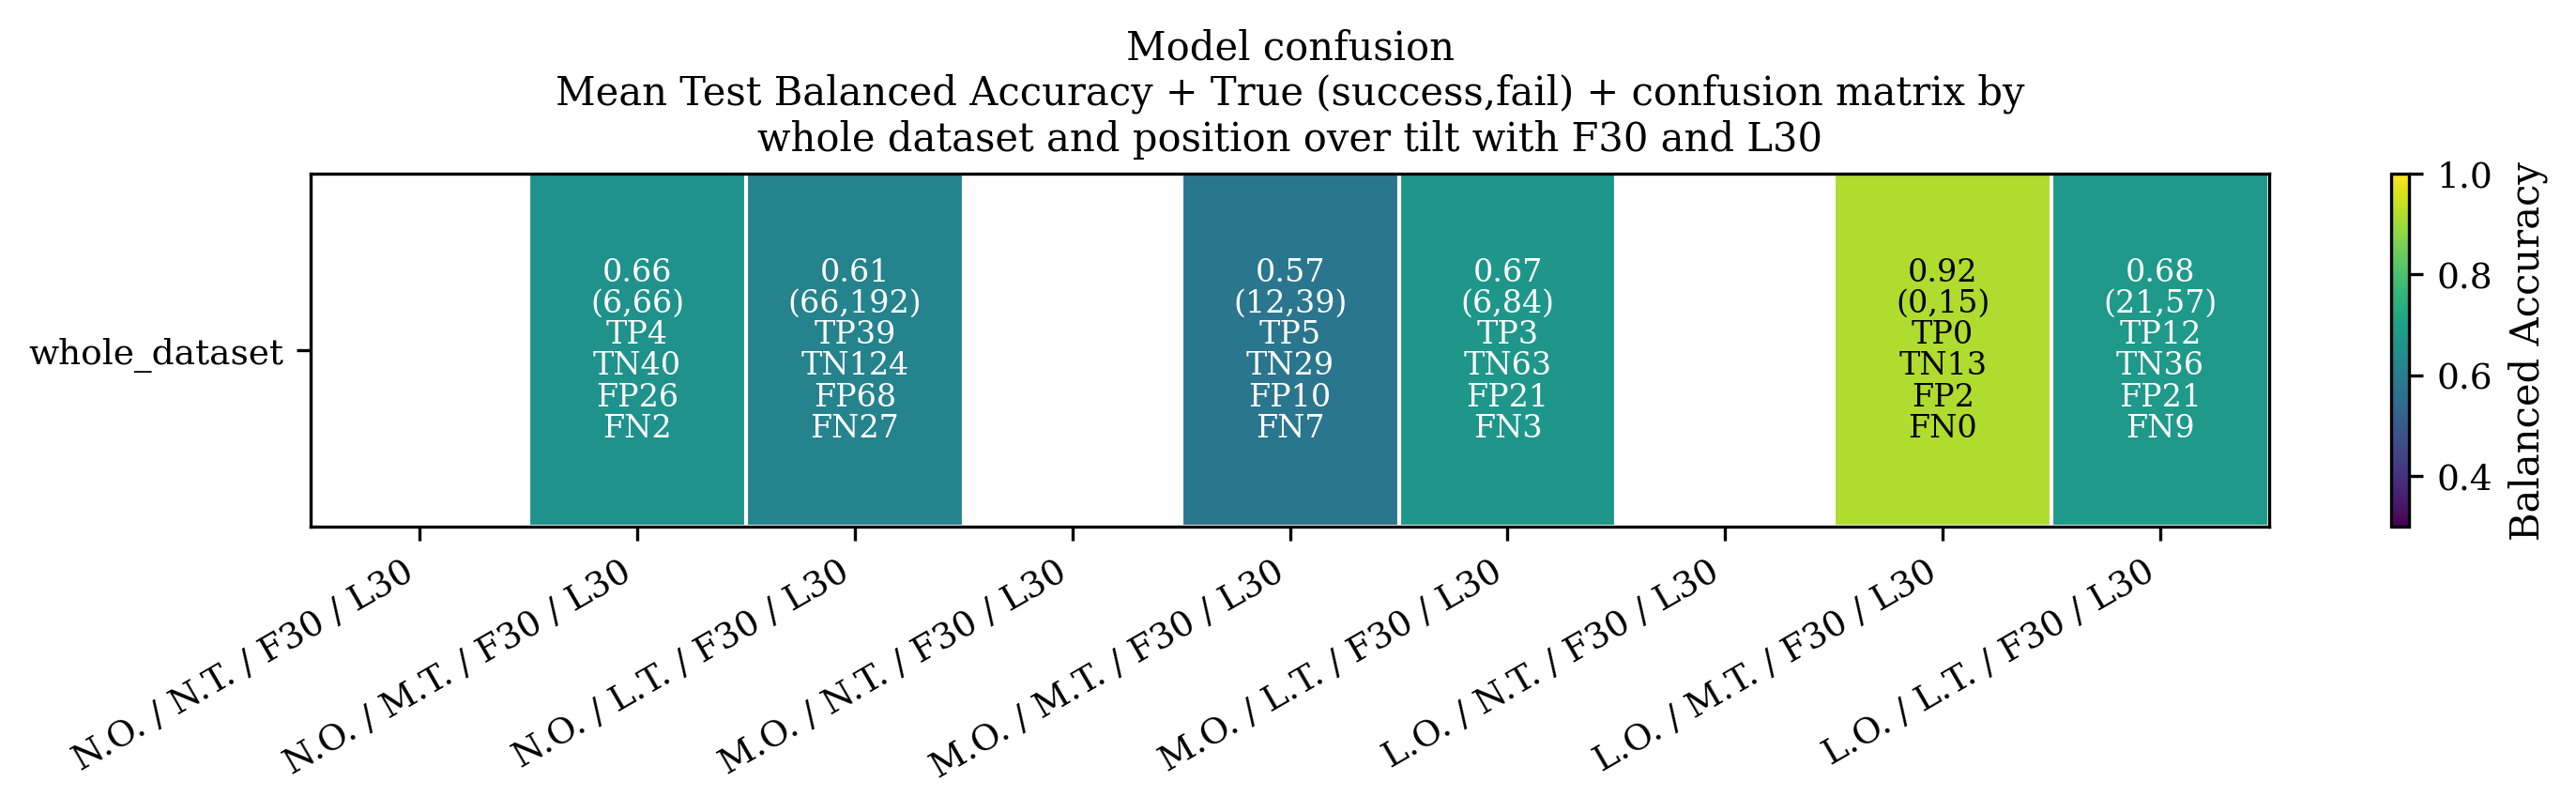
\includegraphics[width=0.95\linewidth]{chapters/7-results_and_discussion/DA2/domain/model_position_over_tilt_F30_L30.png}
    \caption{Model balanced accuracy for combined position--tilt groups within the force-interaction group \texttt{F30/L30}. Tile annotations show the true class split and confusion-matrix entries.}
    \label{fig:da2_position_tilt_f30_l30}
\end{figure}

\begin{figure}[htbp]
    \centering
    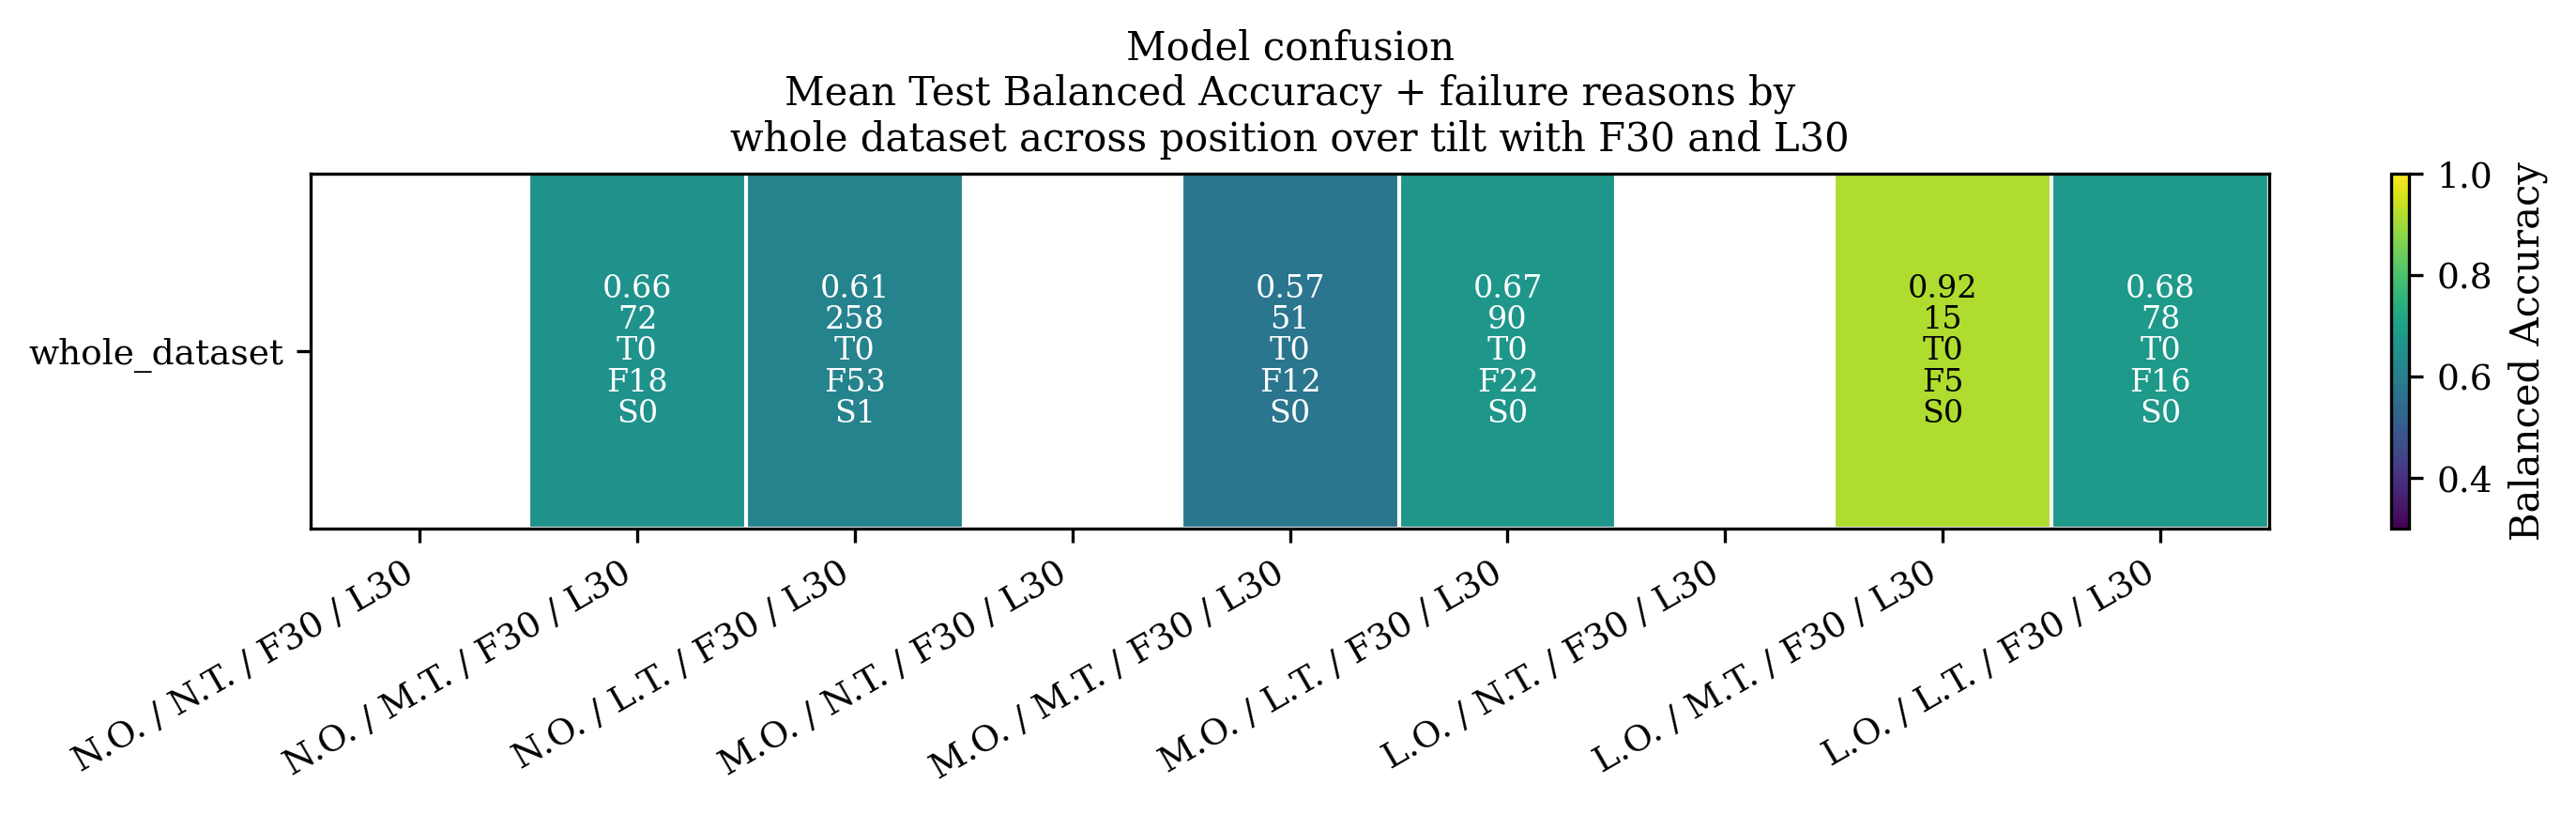
\includegraphics[width=0.95\linewidth]{chapters/7-results_and_discussion/DA2/domain/model_position_over_tilt_F30_L30_failure_reasons.png}
    \caption{Model balanced accuracy for combined position--tilt groups within the force-interaction group \texttt{F30/L30}. Tile annotations show the physical failure reasons entries.}
    \label{fig:da2_position_tilt_f30_l30_failure_reason}
\end{figure}

\subsubsection{Small-Sample Outlier in \texttt{rect\_rod\_t0.2}}
\label{subsubsec:da2_rect_rod_t02_outlier}

\figref{fig:da2_rect_rod_t02_position_tilt_all_holes} shows the test balanced accuracy for all hole domains across all position over tilt deviation groups. One particular case stands out for \texttt{rect\_rod\_t0.2} on \texttt{N.O./N.T.}, where the balanced accuracy is really low only in one cell with neighboring cells showing normal behavior. At first, this cell appears to indicate that a no-offset/no-tilt combination is highly confusing for the model in the specific \texttt{rect\_rod\_t0.2}. However, further analysis in \figref{fig:da2_rect_rod_t02_position_tilt} with detailed annotation, shows that the group contains only 18 prediction records, with a true class split of 9 successful and 9 failed insertions. Of these, 10 predictions are incorrect.
Because of the very low sample count, compared to the other groups with 100 to 200 samples each, this case is therefore treated as a local outlier.

\begin{figure}[htbp]
    \centering
    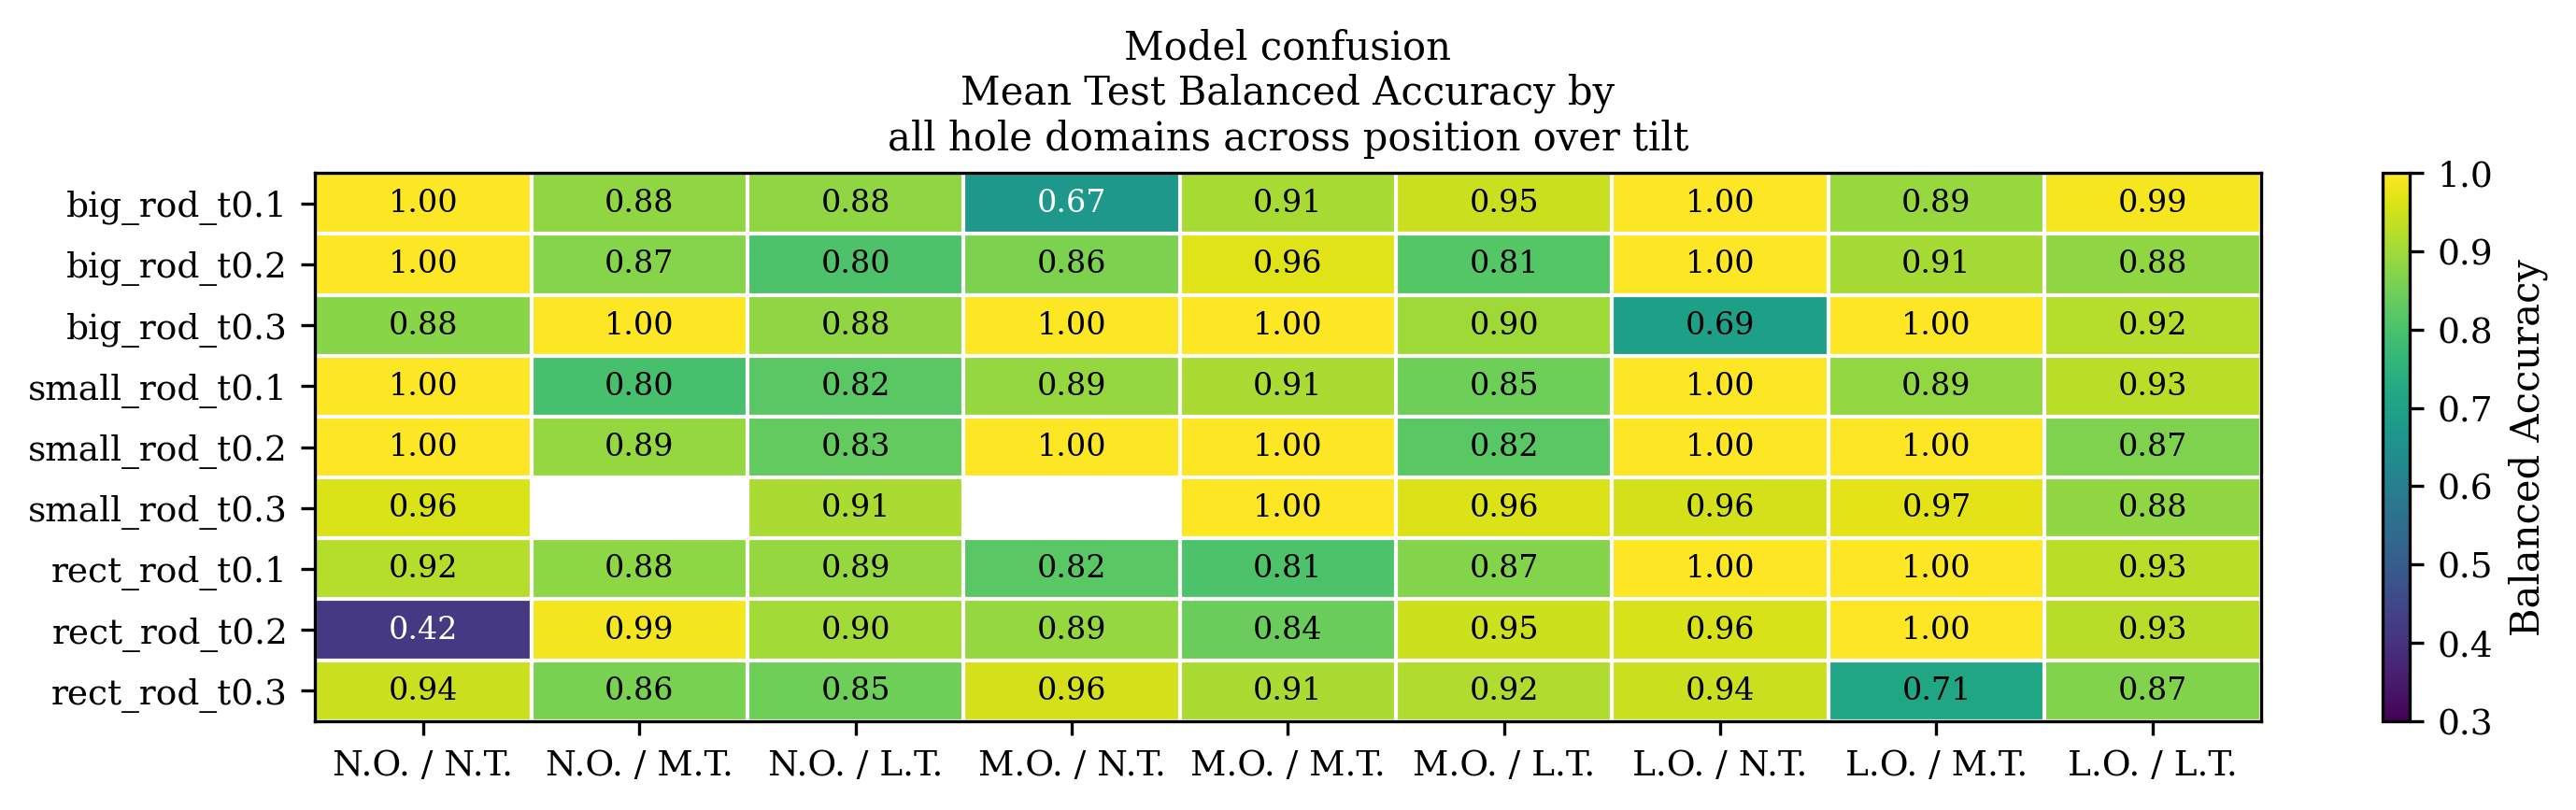
\includegraphics[width=0.95\linewidth]{chapters/7-results_and_discussion/DA2/domain/model_hole_domain_position_over_tilt.png}
    \caption{Model balanced accuracy for combined position--tilt groups over all hole domains.}
    \label{fig:da2_rect_rod_t02_position_tilt_all_holes}
\end{figure}

\begin{figure}[htbp]
    \centering
    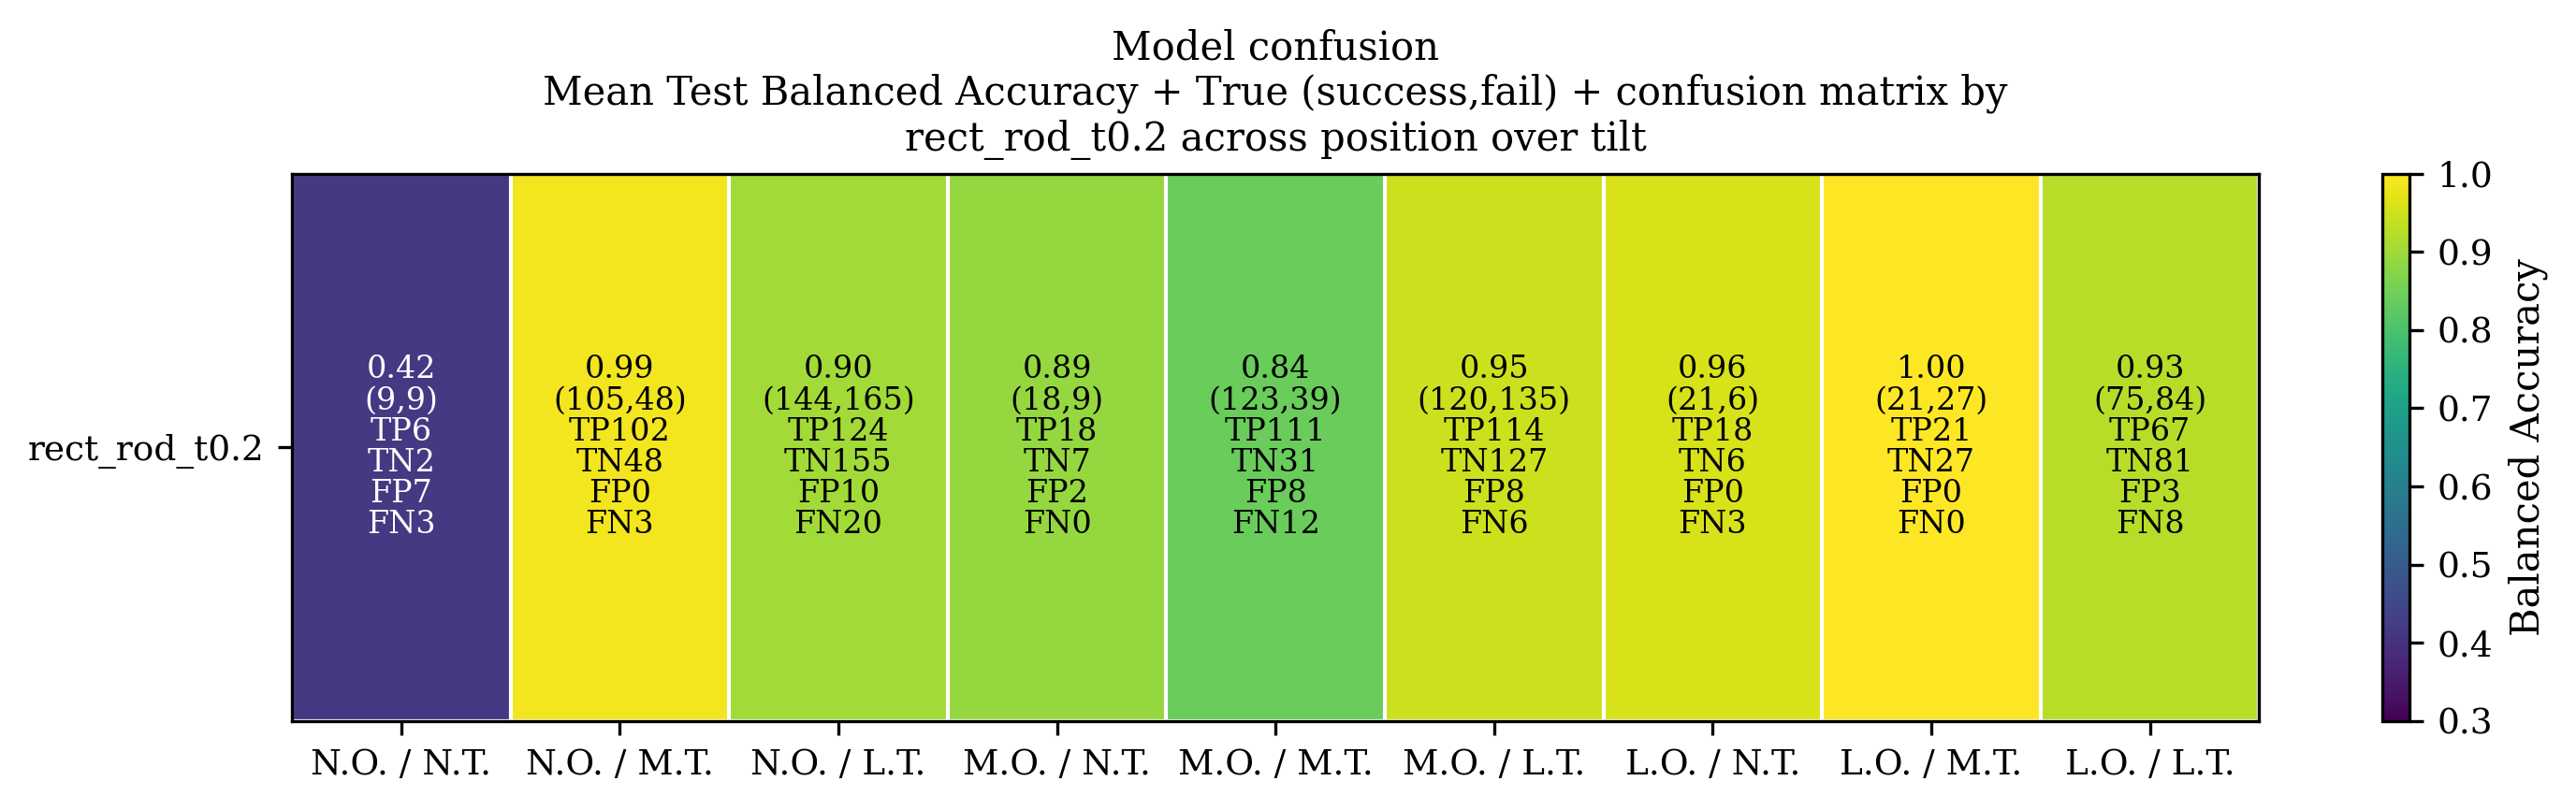
\includegraphics[width=0.95\linewidth]{chapters/7-results_and_discussion/DA2/domain/model_rect_rod_t0.2_domain_position_over_tilt.png}
    \caption{Detailed model balanced accuracy for combined position--tilt groups in the \texttt{rect\_rod\_t0.2} domain. Tile annotations show the true class split and confusion-matrix entries.}
    \label{fig:da2_rect_rod_t02_position_tilt}
\end{figure}

\subsubsection{Directional Model Confusion in \texttt{small\_rod\_t0.3}}
\label{subsubsec:da2_small_rod_t03_direction}

The offset-direction heatmap in \figref{fig:da2_domain_offset_direction_holes} shows that offset direction is not a major global source of model confusion, but it does reveal a domain-specific effect in \texttt{small\_rod\_t0.3}. This is consistent with Deviation Analysis I, where the same domain showed a strong physical directional bias for negative offset directions.

The detailed plot in \figref{fig:da2_small_rod_t03_negx_position_tilt} shows that the reduced balanced accuracy in the negative $x$ direction is mainly caused by the large-offset/large-tilt group. This group contains 78 prediction records, with 18 true successful and 60 true failed insertions. The confusion matrix shows that most failed insertions are correctly classified (TN57), while most successful insertions are missed (FN16). In other words, the model learns that this region normally almost always fails, and therefore struggles to recognize the rare successful exceptions.

This result is similar to the global behavior observed for \texttt{F40/L30} in \figref{fig:da2_model_force_interaction_global} and \figref{fig:da2_model_loss_force_interaction_global}, where a physically difficult group with a strong failure majority can lead the model to predict failure for nearly all samples. Such cases are important because they show that model confusion is not always caused by uncertainty between two equally likely classes. It can also occur when a deviation group is highly imbalanced, because it failes very often, and the rare successful cases do not produce sufficiently distinct signal patterns, which supports the earlier claim.

\begin{figure}[htbp]
    \centering
    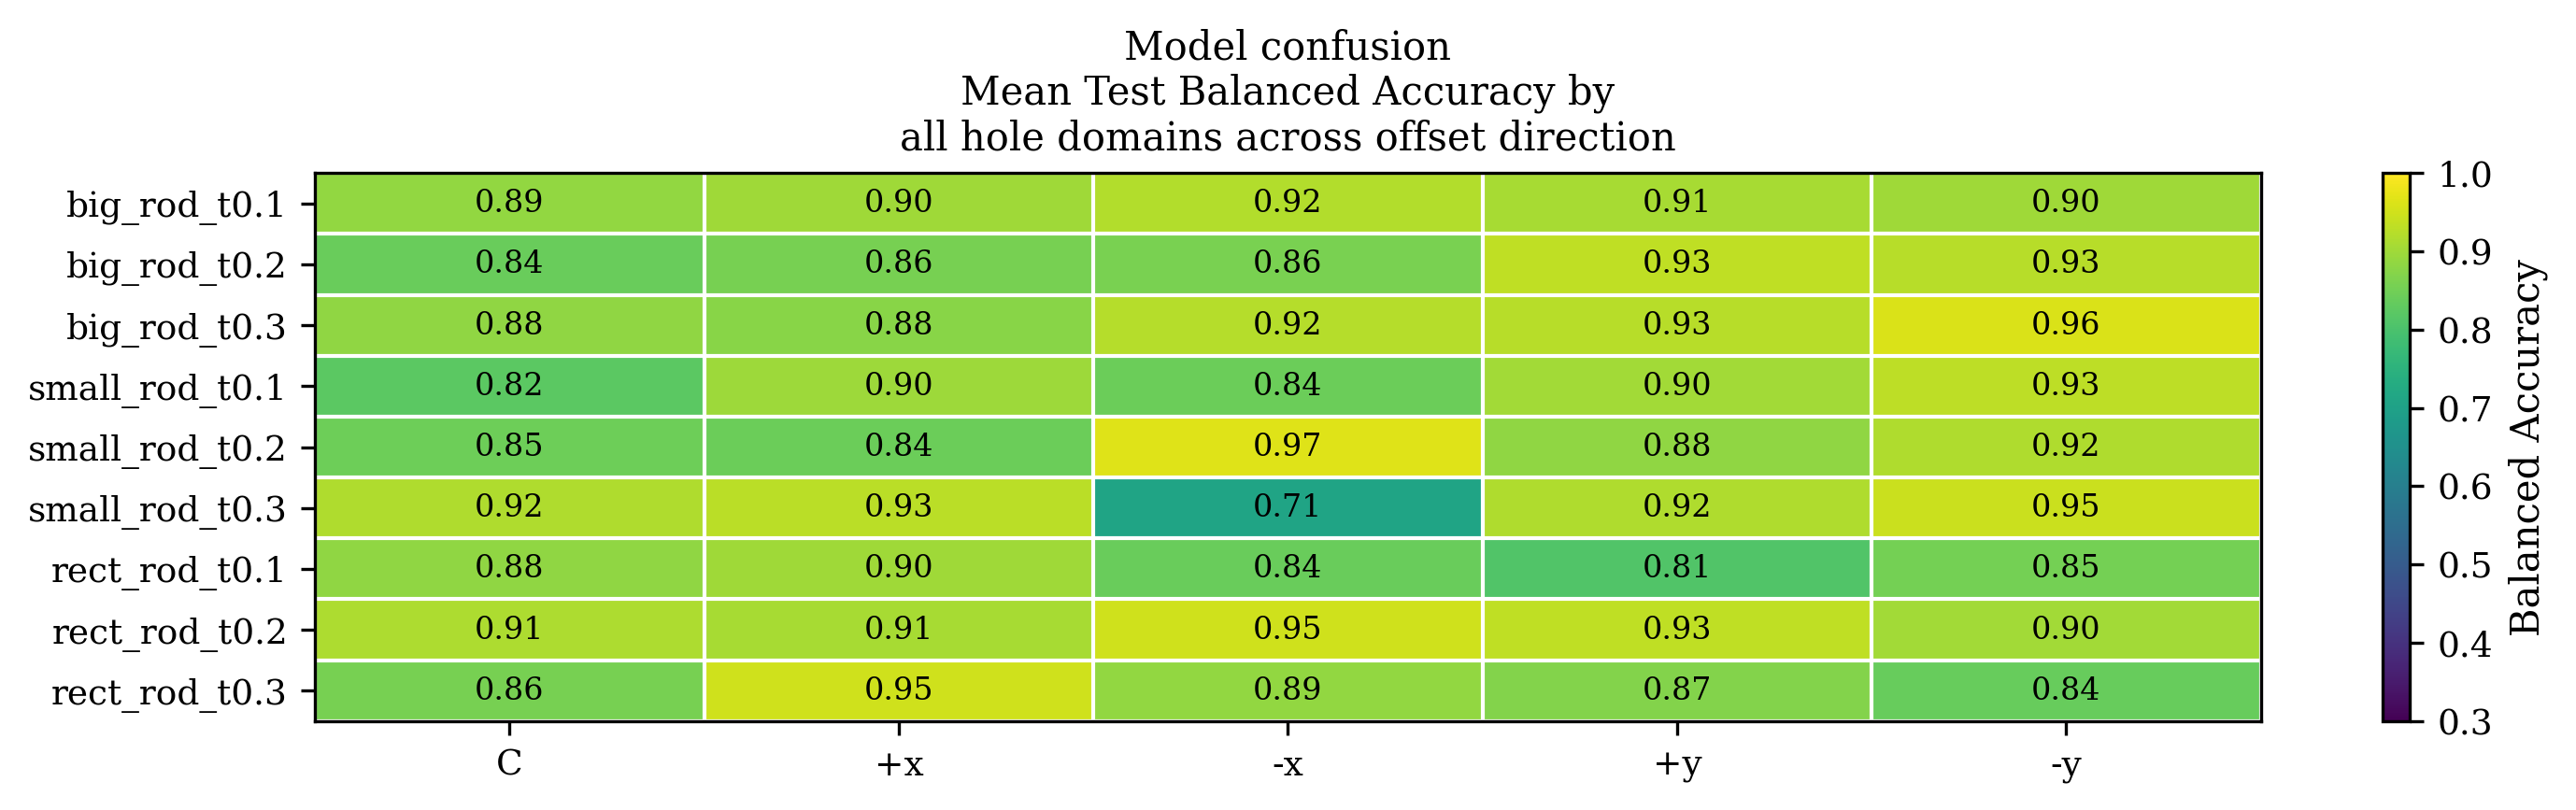
\includegraphics[width=0.95\linewidth]{chapters/7-results_and_discussion/DA2/domain/model_hole_domain_offset_direction.png}
    \caption{Domain-specific model balanced accuracy for offset-direction groups across hole domains.}
    \label{fig:da2_domain_offset_direction_holes}
\end{figure}

\begin{figure}[htbp]
    \centering
    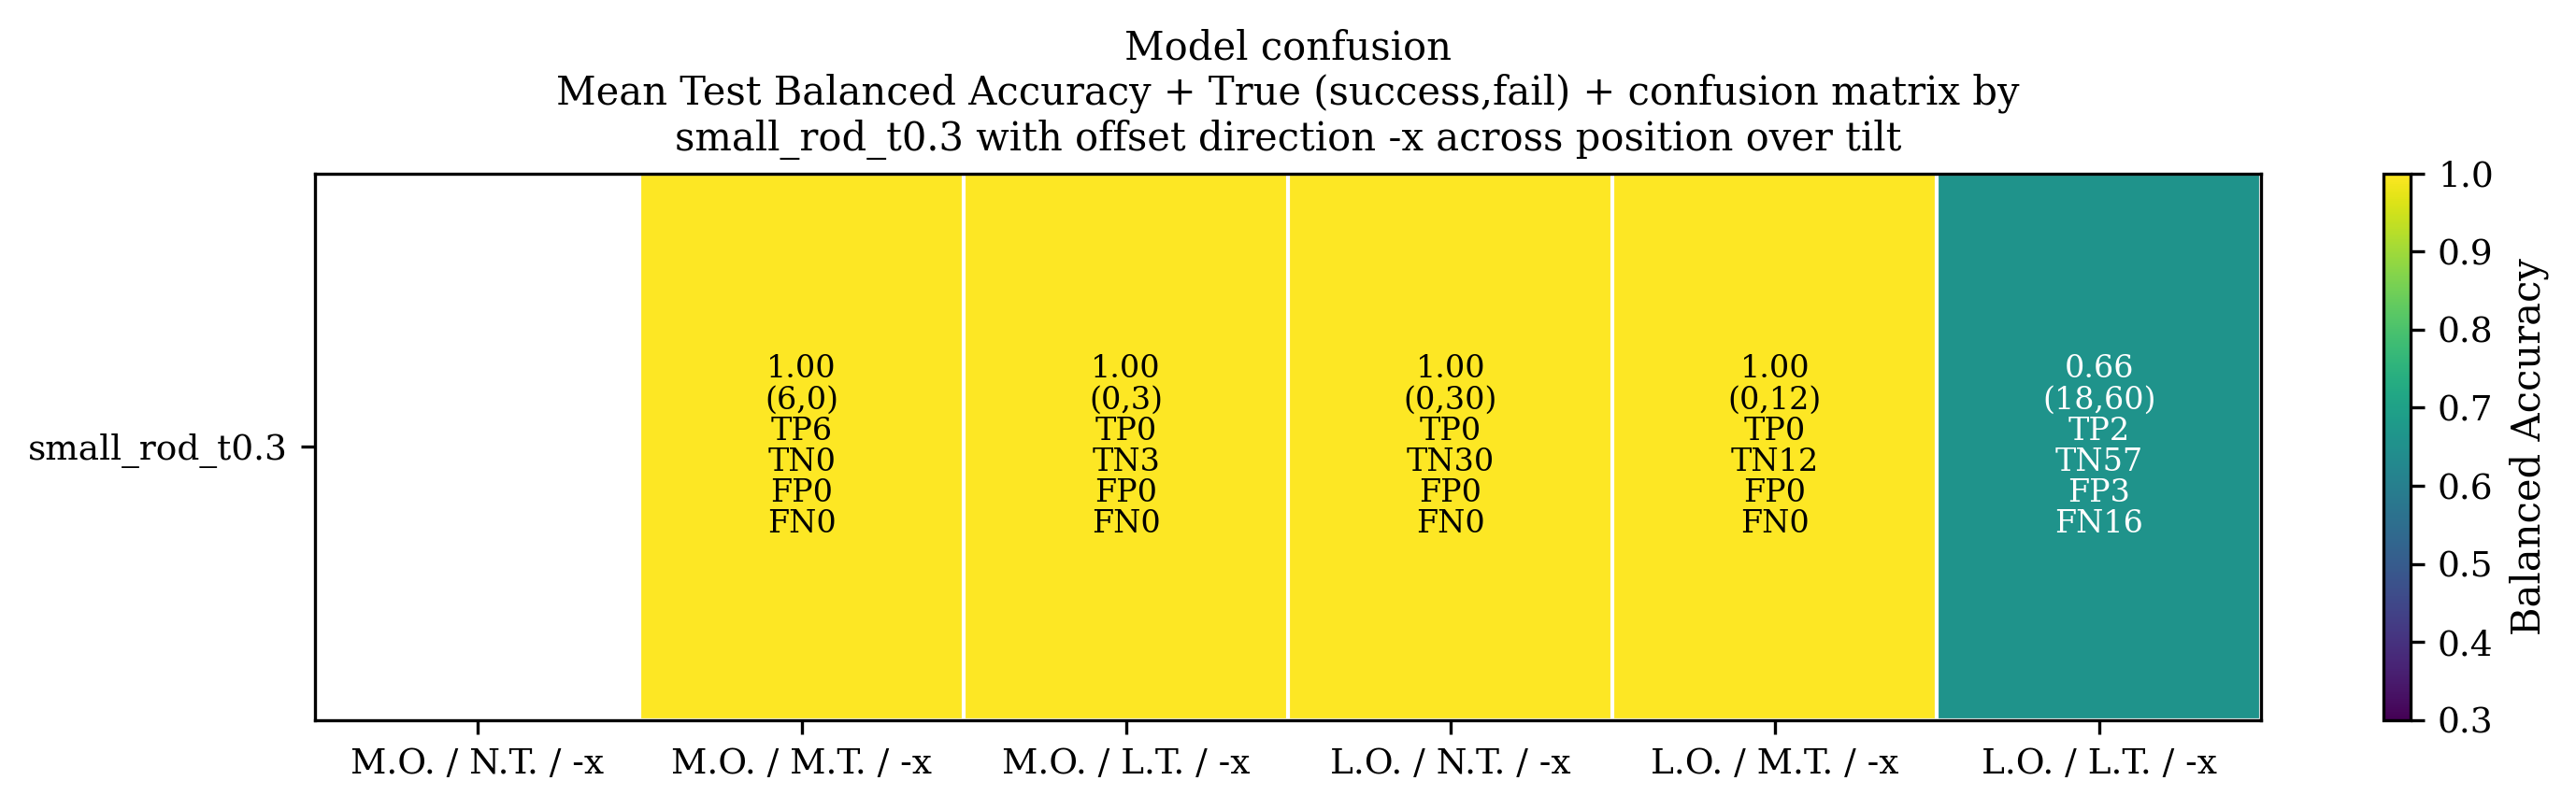
\includegraphics[width=0.95\linewidth]{chapters/7-results_and_discussion/DA2/domain/model_small_rod_t0.3_offset_direction_position_over_tilt.png}
    \caption{Detailed model balanced accuracy for the negative $x$ offset direction in \texttt{small\_rod\_t0.3}, separated by combined position--tilt groups. Tile annotations show the true class split and confusion-matrix entries.}
    \label{fig:da2_small_rod_t03_negx_position_tilt}
\end{figure}

\subsubsection{Summary of Deviation Analysis II}
\label{subsubsec:da2_summary}

The model-confusion analysis shows that physical difficulty and classification difficulty are related, but not identical. In Deviation Analysis I, large tilt clearly reduced the physical success rate. In Deviation Analysis II, however, the large-tilt groups still reach comparatively high balanced accuracy. This indicates that many physically failed insertions caused by large tilt produce signal patterns that are recognizable for the model. Therefore, a deviation can be physically unfavorable without necessarily being model-confusing.

The strongest model-confusion effects are found in the force-interaction groups. In particular, force settings with a small or negative difference between force limit and force level lead to reduced balanced accuracy. The most extreme example is \texttt{F40/L30}. This group is physically almost always unsuccessful, and the model therefore predicts the dominant failure class reliably. However, the few successful exceptions are missed, which results in a false-negative rate of 1.0. Other groups, such as \texttt{F30/L30} and \texttt{F40/L40}, show both low balanced accuracy and high loss. A high loss comes from penalizing high confidence to the wrong classes, or low probability to the true class. These groups are not only wrong classified after thresholding, but are confidentially wrong, indicating genuinely ambiguous or inconsistent signal patterns.

A central observation is that the physical success rate of a deviation group inherently determines the local class balance available for learning and evaluation. A success rate close to 50\% is physically not desirable, but it provides a comparatively balanced distribution of successful and failed insertions. This can be favorable for the classifier, because both classes are sufficiently represented within the group. In contrast, the physically desirable case of almost 100\% success and the physically undesirable case of almost 0\% success both lead to highly imbalanced classes. In these extreme cases, the model tends to learn the dominant outcome and struggles with the rare exceptions. This explains why physically easy groups such as \texttt{N.O./N.T.} can still show increased false-positive rates, while physically difficult groups such as \texttt{F40/L30} or the negative-$x$ large-offset/large-tilt group of \texttt{small\_rod\_t0.3} show increased false-negative behavior.

The domain-specific analysis supports this interpretation. The detailed inspection of \texttt{F30/L30} shows that its low performance is not caused by one isolated position--tilt group. Instead, the group remains ambiguous across several available position--tilt combinations and is dominated by force-limit-related failures. The \texttt{rect\_rod\_t0.2} no-offset/no-tilt case demonstrates the importance of sample count: a very low balanced accuracy in a single heatmap cell can result from only a small number of prediction records and should not be interpreted as a global domain effect. In contrast, the \texttt{small\_rod\_t0.3} negative-$x$ case connects directly to the physical directional bias found in Deviation Analysis I. The model correctly classifies most failures in the large-offset/large-tilt subgroup, but misses most of the rare successful insertions. This shows that the model captures the dominant failures associated with this subgroup, but does not reliably identify successful exceptions.

The record-offset groups show no severe global performance collapse. This indicates that the final model is reasonably robust to the tested temporal shifts of the recorded sequence window. Likewise, offset direction is not a major global source of model confusion, even though it revealed physical setup asymmetries in the success-rate analysis.

Overall, Deviation Analysis II shows that the final PatchTST model using the best channels is robust across most deviation groups and domains. The main classification weaknesses occur in locally imbalanced deviation- or force-limit-related groups, where the signal patterns of rare exceptions are not sufficiently distinct from the dominant outcome.

% \section{Summary of Main Findings}
% \label{sec:results_summary}